\documentclass[12pt]{article}
\usepackage[utf8]{inputenc}
\usepackage[greek,english]{babel}
\usepackage{graphicx}
\usepackage{fontspec}
\setmainfont{Times New Roman} % Μπορούσα και GFS Didot
\usepackage[a4paper, margin=2.5cm]{geometry}
\usepackage{setspace}
\onehalfspacing
\usepackage{titlesec}
\usepackage{titling}
\usepackage{fancyhdr}
\usepackage{amsmath}
\usepackage{array}
\usepackage{emptypage}
\usepackage{lipsum}
\usepackage{xcolor}
\usepackage{hyperref} 
\usepackage{tocloft}      
\usepackage{url}
\numberwithin{equation}{section}
\usepackage{amssymb}
\usepackage{makecell}   % για σπασίματα γραμμών σε κελί
\usepackage{float}

\renewcommand{\cellalign}{tl}

\selectlanguage{greek}

\begin{document}
\thispagestyle{empty}
\begin{center}
    \includegraphics[width=0.185\textwidth]{images/ntua_logo.png} \\ % Make sure the logo image exists here
    \noindent\rule{0pt}{1.5em}


    \textbf{\Large ΕΘΝΙΚΟ ΜΕΤΣΟΒΙΟ ΠΟΛΥΤΕΧΝΕΙΟ} \\[0.5em]
    Σχολή Εφαρμοσμένων Μαθηματικών και Φυσικών Επιστημών \\[0.5em]
    Τομέας Μαθηματικών \\[3em]

\vspace{1.9cm} 

    {\selectlanguage{english}
    
    \textbf{\Large Panoptic Segmentation with Deep Neural Networks} \\[2em]
    }

    \textbf{\LARGE ΔΙΠΛΩΜΑΤΙΚΗ ΕΡΓΑΣΙΑ} \\[1.5em]

    του \\
    \textbf{Νικόλα Ιωάννου} \\[4em]

\vspace{1.8cm} 


\hspace*{-0.3cm}\textbf{Επιβλέπων:} Παναγιώτης Τσανάκας       \hspace*{3.65cm} \textbf{Συνεπιβλέπων:} Γεώργιος Σιόλας \\
\hspace*{1.76cm}Καθηγητής Ε.Μ.Π.  \hspace*{7.23cm}Ε.ΔΙ.Π. Ε.Μ.Π.

\vspace{5.5 cm} 






    \scalebox{0.9}{ΕΡΓΑΣΤΗΡΙΟ ΟΡΑΣΗΣ ΥΠΟΛΟΓΙΣΤΩΝ, ΕΠΙΚΟΙΝΩΝΙΑΣ ΛΟΓΟΥ ΚΑΙ ΕΠΕΞΕΡΓΑΣΙΑΣ ΣΗΜΑΤΩΝ} 
 \\
    \scalebox{1}{Αθήνα, Ιούλιος 2025}
\end{center}
\pagenumbering{roman}
\newpage
\mbox{}
\newpage

\begin{center}
\noindent
\begin{minipage}{0.2\textwidth}
    \hspace*{10pt} %
    \includegraphics[width=2.8cm,height=2.8cm]{images/ntua_logo.png} % Adjust path if needed
\end{minipage}
\hfill
\begin{minipage}{0.75\textwidth}
    \selectlanguage{greek}
    \small % or \footnotesize or any other size you want
    \textbf{Εθνικό Μετσόβιο Πολυτεχνείο}\\[-2pt]
    Σχολή Εφαρμοσμένων Μαθηματικών και Φυσικών Επιστημών\\[-2pt]
    Τομέας Μαθηματικών\\[-2pt]
    Εργαστήριο Όρασης Υπολογιστών, Επικοινωνίας Λόγου και Επεξεργασίας Σημάτων
\end{minipage}


\vspace{2.5cm} 

    {\selectlanguage{english}
    
    \textbf{\Large Panoptic Segmentation with Deep Neural Networks} \\[2em]
    }

    \textbf{\LARGE ΔΙΠΛΩΜΑΤΙΚΗ ΕΡΓΑΣΙΑ} \\[1.5em]

    του \\
    \textbf{Νικόλα Ιωάννου} \\[4em]

\vspace{0.6cm} 


\hspace*{-0.3cm}\textbf{Επιβλέπων:} Παναγιώτης Τσανάκας       \hspace*{3.65cm} \textbf{Συνεπιβλέπων:} Γεώργιος Σιόλας \\
\hspace*{1.76cm}Καθηγητής Ε.Μ.Π.  \hspace*{7.23cm}Ε.ΔΙ.Π. Ε.Μ.Π.

\vspace{2.5cm}
{\raggedright \small Εγκρίθηκε από την τριμελή εξεταστική
 επιτροπή την 1η Ιουλίου, 2025. \\
 
 }

\vspace{2cm}

(Υπογραφή)\hspace*{4cm} (Υπογραφή)\hspace*{4cm} (Υπογραφή)\\
\vspace{0.8 cm} 
.................... \hspace*{4cm} ....................\hspace*{4cm}  ....................\\
Παναγιώτης Τσανάκας\hspace*{2.4cm}  Αντώνιος Συμβώνης\hspace*{3cm}  Γεώργιος Στάμου \\
 Καθηγητής Ε.Μ.Π.\hspace*{3cm} 	 Καθηγητής Ε.Μ.Π.\hspace*{3cm}  Καθηγητής Ε.Μ.Π. 


\vspace{2.9 cm} 






    \scalebox{1}{Αθήνα, Ιούλιος 2025}
\end{center}

\newpage

\vspace*{\fill}
	{\raggedleft ........................................\\
    \textbf ΙΩΑΝΝΟΥ ΝΙΚΟΛΑΣ\\
    \textit{Διπλωματούχος σχολής Εφαρμοσμένων\\
    Μαθηματικών και Φυσικών Επιστημών Ε.Μ.Π.}
    
    }

\vspace*{\fill}


\vspace{2cm}
{
\small
\noindent \textcolor{black}{\textcopyright{} -- All rights reserved. Με επιφύλαξη παντός δικαιώματος.\\ Νικόλας Ιωάννου, 2025.}\\


\vspace{0.1cm}


\noindent\textcolor{black}{ Απαγορεύεται η αντιγραφή, αποθήκευση και διανομή της παρούσας εργασίας, εξ ολοκλήρου ή τμήματος αυτής, για
εμπορικούς σκοπούς. Επιτρέπεται η ανατύπωση, αποθήκευση και διανομή για σκοπούς μη κερδοσκοπικούς, εκπαιδευτικής
ή ερευνητικής φύσης, υπό την προϋπόθεση να αναφέρεται η πηγή προέλευσης και να διατηρείται το παρόν μήνυμα. Ερωτήματα που αφορούν τη χρήση της εργασίας για κερδοσκοπικό σκοπό πρέπει να απευθύνονται προς τον
συγγραφέα.
}

\vspace{0.1cm}

\noindent \textcolor{black}{ Οι απόψεις και τα συμπεράσματα που περιέχονται σε αυτό το έγγραφο εκφράζουν τον συγγραφέα και δεν πρέπει
να ερμηνευθεί ότι αντιπροσωπεύουν τις επίσημες θέσεις του Εθνικού Μετσόβιου Πολυτεχνείου.}}

\newpage
\mbox{}
\newpage

\section*{Περίληψη}
Στην


\newpage
\mbox{}
\newpage

\section*{Abstract}
in



\newpage
\mbox{}
\newpage

\section*{Ευχαριστίες}
Θα ήθελα να ευχαριστήσω τον κ.Γεώργιο Σιόλα για την επίβλεψη της παρούσας διπλωματικής εργασίας. Θα ήθελα να ευχαριστήσω επίσης την οικογένεια μου γιατί χωρίς αυτούς δεν θα μπορούσα να βρίσκομαι στην θέση την οποία βρίσκομαι τώρα.


\newpage
\mbox{}
\newpage


\tableofcontents

\newpage
\listoffigures
\addcontentsline{toc}{part}{List of Figures}

\newpage
\listoftables
\addcontentsline{toc}{part}{List of Tables}

\newpage
\pagenumbering{arabic}


\section{Εισαγωγή}

\newpage

\section{Ορισμός και περιγραφή του προβλήματος}

Η όραση υπολογιστών αποτελεί προσομοίωση της βιολογικής όρασης, κάνοντας χρήση υπολογιστών και συναφούς εξοπλισμού.Αποσκοπεί στην κατανόηση της τρισδιάστατης δομής του περιβάλλοντος, μέσω της επεξεργασίας εικόνων και βίντεο και έχει ως απότερο σκοπό την κατανόηση του οπτικού περιεχομένου. Το πεδίο αυτό περιλαμβάνει μεταξύ άλλων την

\begin{itemize}
    \item Επεξεργασία εικόνας (Image Processing)
    \item Αναγνώριση προτύπων (Pattern Recognition)
    \item Γεωμετρική μοντελοποίηση (Geometric modeling)
    \item Αναγνώριση αντικειμένων (Recognition Processes)
\end{itemize}

\noindent ~\cite{Gao_2020}. Η όραση υπολογιστών μπορεί να εφαρμοσθεί σε μια ευρύα γκάμα αντικειμένων όπως η ιατρική στον εντοπισμό κακοήθη όγκου~\cite{Esteva2021}, στην αυτόνομη οδήγηση για την κατανόηση του περιβάλλοντος γύρω του οχήματος~\cite{unknown1} και στην ρομποτική~\cite{article1}. \\

Η ιστορική της πορεία ξεκινά στις αρχές της δεκαετίας του 1960 όταν η έρευνα επικεντρώθηκε σε βασικές τεχνικές επεξεργασίας εικόνας, όπως το φιλτράρισμα (Filtering), η οριοθέτηση και η ανίχνευση ακμών. Αρχικά ο στόχος ήταν η ανάλυση των τιμών των εικονοστοιχείων, όπως και η αναγνώριση απλών σχημάτων. Κατά την διάρκεια της δεκαετίας του 1980 αναπτύχθηκαν πιο σύνθετες τεχνικές που επέτρεπαν την αναγνώριση πιο σύνθετων σχημάτων και την εξαγωγή χαρακτηριστικών. Τη δεκαετία του 1990 η όραση υπολογιστών πέρασε στην φάση της μηχανικής μάθησης, όπου υιοθετήθηκαν στατιστικές μεθόδοι όπως για παράδειγμα μεθόδοι που έκαναν χρήση μηχανών διανυσμάτων υποστήριξης (Support Vector Machines) και τυχαίων δασών (Random Forest). Σημείο καμπής αποτέλεσε η δεκαετία του 2010 όπου με την τεράστια πρόοδο της υπολογιστικής ισχύς και την δημιουργία συνόλων δεδομένων μεγάλου μεγέθους με τις κατάλληλες επισημειώσεις, άνοιξε την πόρτα σε αλγορίθμους βασισμένους στην βαθιά μάθηση και συγκεκριμένα στα νευρωνικά δίκτυα και τα συνελικτικά νευρωνικά δίκτυα, οι οποίοι σημείωσαν τεράστια πρόοδο. Σημαντικό παράδειγμα σε αυτό αποτέλεσε το AlexNet~\cite{NIPS2012_c399862d}, ένα βαθύ συνελικτικό νευρωνικό δίκτυο που κατασκέυασε ο Geoffrey E. Hinton με την ομάδα του, το οποίο πέτυχε 15.3\% top-5 error rate στο ILSVRC (ImageNet
Large Scale Visual Recognition Challenge)~\cite{russakovsky2015imagenetlargescalevisual}. Σήμερα, η όραση υπολογιστών επικεντρώνεται κυρίως στην ανάπτυξη μοντέλων που μπορούν να εξάγουν αποτελέσματα σε πραγματικό χρόνο, χωρίς αισθητή χρονική καθυστέρηση, σε ηθικά ζητήματα όπως η αμεροληψία των αποτελεσμάτων όπως και σε ζητήματα ιδιωτικότητας~\cite{article2}. \\

Η όραση υπολογιστών περιλαμβάνει μια πληθώρα εργασιών, κάθε μια με διαφορετικό σκοπό και επίπεδο ανάλυσης της οπτικής πληροφορίας~\cite{boesch2024computer}, ~\cite{zhou2024comprehensive}. Μεταξύ άλλων έχουμε την

\begin{itemize}
    \item Κατάτμηση εικόνας (Image Segmentation)
    \item Ταξινόμηση εικόνας (Image Classification)
    \item Ανίχνευση αντικειμένων (Object Detection)
    \item Ανακατασκευή τρισδιάστασης εικόνας (3 Dimensional Image Reconstruction)
    \item Εκτίμηση βάθους (Depth Estimation) 
\end{itemize}


\subsection{Κατάτμηση εικόνας}

Η κατάτμηση εικόνας αποτελεί τεχνική στην όραση υπολογιστών που περιλαμβάνει την διαίρεση εικόνων ή βίντεο σε πλήθος αντικειμένων ή περιοχών. Κατά την διάρκεια των ετών έχουν αναπτυχθεί πολυάριθμοι αλγόριθμοι που προσπαθούν να αντιμετωπίσουν το συγκεκριμένο πρόβλημα με κάποιους απο τους πιο αρχικούς να βασίζονται σε μεθόδους κάνοντας χρήση κατωφλίου (Threshhold), ομαδοποίησης βάση ιστογράμματος, ομαδοποίησης μέσω του K-means όπως και σε πιο προχωρημένους όπως αλγορίθμους όπως οι ενεργές καμπύλες (active contours) , οι τομές γράφων, στα υπο συνθήκη και τυχαία πεδία Markov όπως και σε αλγορίθμους βασισμένους στην αραιότητα.Κατατάλλα, τα τελευταία χρόνια τα μοντέλα βαθιάς μάθησης(Deep learning models) έχουν οδηγήσει σε μια νεα γενιά μοντέλων κατάτμησης εικόνας με εντυπωσιακές αποδόσεις, συχνά επιτυγχάνοντας τις υψηλότερες αποδόσεις σε διάσημα σύνολα αναφοράς (Benchmarks)~\cite{DBLP:journals/corr/abs-2001-05566}. Χωρίζεται σε κατηγορίες όπως 

\begin{itemize}
    \item Σημασιολογική κατάτμηση εικόνας (Semantic Image Segmentation)
    \item Κατάτμηση αντικειμένων (Instance Segmentation)
    \item Πανοπτική κατάτμηση εικόνας (Panoptic Image Segmentation)
\end{itemize}

\subsubsection{Σημασιολογική κατάτμηση εικόνας}

Ζητούμενο της σημασιολογικής κατάτμησης εικόνας είναι ο προσδιορισμός της σημασιολογικής κατηγορίας κάθε εικονοστοιχείου μιας εικόνας. Κατά κανόνα, το πρόβλημα αποτελεί πρόβλημα επιπτεβόμενης μάθησης (Supervised learning), αξιοποιώντας ένα σύνολο εικόνων όπου κάθε εικόνα είναι επισυμασμένη σε επίπεδο εικονοστοιχείου, με σκοπό την εκπαίδευση ενός μοντέλου για την εκτέλεση του έργου. Οι σημασιολογικές ετικέτες χωρίζονται σε δύο κατηγορίες, στα "αντικείμενα" (Things), όπως για παράδειγμα σκύλος, αυτοκίνητο, πεζός κ.ο.κ. και στα "σκηνικά" στοιχεία (Stuff), όπως για παράδειγμα ουρανός, βλάστηση, δρόμος κ.ο.κ. Οι δύο αυτοί όροι χρησιμοποιούνται εκτενώς στην κατάτμησης εικόνας . Η πρώτη κατηγορία αναφέρετε σε μετρήσιμα αντικείμενα, ενώ η δεύτερη κατηγορία σχετίζεται με στοιχεία του σκηνικού~\cite{csurka2023semanticimagesegmentationdecades}. Παρακάτω παρουσιάζεται μια αναπαράσταση της συγκεκριμένης τεχνικής.

\begin{figure}[h!]
  \centering
  \includegraphics[width=0.60\textwidth]{images/figure0.png} % replace with your image file name
  \caption{Αυθεντική εικόνα}
  \label{figure 1}
\end{figure}

\begin{figure}[h!]
  \centering
  \includegraphics[width=0.6\textwidth]{images/figure1.png} % replace with your image file name
  \caption{Σημασιολογική κατάτμηση εικόνας}
  \label{figure 2}
\end{figure}

Όπως μπορούμε να δούμε στην εικόνα κάθε εικονοστοιχείο της αντιστοιχείζεται σε κάποια σημασιολογική κατηγορία. Μπορούμε να παρατηρήσουμε πως τα εικονοστοιχεία που αντιστοιχείζονται στην ίδια σημασιολογική κατηγορία είναι τα εικονοστοιχεία τα οποία αντιστοιχούν στο ίδιο "αντικείμενο" ή "σκηνικό" στοιχείο. \\

Σημαντικές μετρικές απόδοσης της σημασιολογικής κατάτμησης εικόνας αποτελούν μεταξύ άλλων οι Intersection over Union (IoU), όπως επίσης και η ακρίβεια εικονοστοιχείου (Pixel Accuracy - PA)~\cite{DBLP:journals/corr/abs-2001-05566}. Μερικά παραδείγματα σημείων αναφοράς (benchmarks) που χρησιμοποιούνται για την ποσοτικοποίηση της απόδοσης συγκεκριμένων αλγορίθμων που χρησιμοποιούν την τεχνική αυτή είναι τα Cityscapes~\cite{DBLP:journals/corr/CordtsORREBFRS16}, PASCAL VOC~\cite{Everingham2010} και ADE20K~\cite{8100027}. \\

\subsubsection{Κατάτμηση αντικειμένων}
Η ανίχνευση αντικειμένων αποτελεί διαδικασία κατά την οποία ο αλγόριθμος εντοπίζει και ταξινομεί τα "αντικείμενα" μιας εικόνας προσδιορίζοντας την θέση τους μέσω ορθογώνιων πλαισίων. Η σημασιολογική κατάτμηση εικόνας, όπως αναφέραμε παραπάνω προσδιορίζει την σημασιολογική κατηγορία κάθε εικονοστοιχείου μιας εικόνας, χωρίς όμως να διαχωρίζει μεταξύ διαφορετικών "αντικειμένων" της ίδιας κατηγορίας. Προχωρώντας ένα βήμα παραπέρα, η κατάτμηση αντικειμένων συνδυάζει αυτές τις 2 τεχνικές και παρέχει διαφορετικές ετικέτες για ξεχωριστές εμφανίσεις "αντικειμένων" που ανήκουν στην ίδια κατηγορία, αγνοώντας εντελώς τα "σκηνικά" στοιχεία~\cite{Hafiz_2020}. \\

\begin{figure}[h!]
  \centering
  \includegraphics[width=0.6\textwidth]{images/figure2.png} % replace with your image file name
  \caption{Κατάτμηση αντικειμένων}
  \label{figure 3}
\end{figure}

Όπως μπορούμε να δούμε στην εικόνα παραπάνω το μοντέλο κατηγοριοποιεί μόνο τα εικονοστοιχεία τα οποία αντιστοιχούν σε "αντικείμενα", αδιαφορώντας για τα υπόλοιπα. Εύκολα μπορούμε να παρατηρήσουμε επίσης πως γίνετε διάκριση μεταξύ των "αντικειμένων" που ανήκουν στην ίδια κατηγορία.\\

Κάποιες απο τις σημαντικόερες μετρικές απόδοσης στην κατάτμηση αντικειμένων αποτελούν οι μέσος όρος ακριβείας (Average Precision) και μέσος όρος ακριβείας μάσκας (Mask AP)~\cite{Hafiz_2020}. Μερικά παραδείγματα συνόλων αναφοράς που χρησιμοποιούνται για την ποσοστικοποίηση της απόδοσης συγκεκριμένων αλγορίθμων που χρησιμοποιούν την τεχνική αυτή είναι τα COCO~\cite{lin2015microsoftcococommonobjects}, Cityscapes~\cite{DBLP:journals/corr/CordtsORREBFRS16} και ADE20K~\cite{8100027}.



\subsubsection{Πανοπτική κατάτμηση εικόνας}

Η πανοπτική κατάτμηση εικόνας αποτελεί διαδικασία κατά την οποία γίνετε συνδυασμός της ανίχνευσης αντικειμένων και της σημασιολογικής κατάτμησης εικόνας. Συγκεκριμένα, στην πανοπτική κατάτμηση εικόνας πραγματοποιήτε κατηγοριοποίηση όλων των εικονοστοιχείων της εικόνας, ανεξάρτητα εάν τα εικονοστοιχεία αντιστοιχούν σε "αντικείμενα" ή "σκηνικά" στοιχεία και παράλληλα γίνετε διαχωρισμός μεταξύ των "αντικειμένων" που αντιστοιχούν στην ίδια σημασιολογική κατηγορία~\cite{elharrouss2021panopticsegmentationreview}.

\newpage

\begin{figure}[h!]
  \centering
  \includegraphics[width=0.6\textwidth]{images/figure3.png} % replace with your image file name
  \caption{Πανοπτική κατάτμηση εικόνας}
  \label{figure 4}
\end{figure}

Όπως μπορούμε να δούμε στην εικόνα παραπάνω το μοντέλο κατηγοριοποιεί όλα τα εικονοστοιχεία της εικόνας και ταυτόχρονα διαχωρίζει τα "αντικείμενα", τα οποία ανήκουν στην ίδια σημασιολογική κατηγορία. \\

Μερικές σημαντικές μετρικές της απόδοσης της πανοπτικής κατάτμησης εικόνας είναι η Panoptic Quality (PQ), η Segmentation Quality (SQ) και η Recognition Quality (RQ). Ωστόσο, γνωρίζουμε πως η πανοπτική κατάτμηση εικόνας αποτελεί συνδυασμό της σημασιολογικής κατάτμησης εικόνας και της κατάτμησης αντικειμένων υπάρχουν μετρικές που έχουν ώς σκοπό την ποσοτικοποίηση της απόδοσης των μοντέλων πανοπτικής κατάτμησης εικόνας στις 2 προηγούμενες εργασίες. Συγκεκριμένα για τα προαναφερθέντα υπάρχουν οι μετρικές απόδοσης Panoptic Quality Things (\(PQ_{th}\)) και Panoptic Quallity Stuff (\(PQ_{st}\))~\cite{elharrouss2021panopticsegmentationreview}. Μερικά παραδείγματα σημείων αναφοράς που χρησιμοποιούνται για την ποσοτικοποίηση της απόδοσης συγκεκριμένων αλγορίθμων που κάνουν χρήση της τεχνικής αυτής είναι τα COCO~\cite{lin2015microsoftcococommonobjects}, Cityscapes~\cite{DBLP:journals/corr/CordtsORREBFRS16} και ADE20K~\cite{8100027}.

\subsection{Συναφή προβλήματα ανάλυσης εικόνας}

Στην παρούσα υπο-ενότητα παρουσιάζονται και αναλύονται συνοπτικά διάφορα προβλήματα της όρασης υπολογιστών, τα οποία καλύπρουν διαφορετικά μέρη της κατανόησης οπτικής πληροφορίας, σε σχέση με την κατάτμηση εικόνας. Η ανάλυση αυτή αποσκοπεί στην σύγκριση της εργασίας της πανοπτικής κατάτμησης εικόνας με διάφορες άλλες εργασίες της όρασης υπολογιστών.\\ 

\paragraph{Ταξινόμηση εικόνας \\ [0.5 cm]}

Η ταξινόμηση εικόνας αποτελεί εργασία στην μηχανική μάθηση κατά την οποία μια εικόνα αντιστοιχίζεται σε μια ή περισσότερες κατηγορίες με βάση το περιεχόμενο της. Έχει εφαρμογή σε ένα ευρύ φάσμα τομέων, όπως η υγεία, η βιομηχανική παραγωγή και η γεωργία~\cite{onix_image_classification_2024}.\\

Κάποιες απο τις σημαντικότερες μετρικές απόδοσης αποτελούν μεταξύ άλλων η ακρίβεια (Accuracy) ταξινόμησης των εικόνων και το F1-score~\cite{article10}, ~\cite{Rainio2024}. Κάποια παραδείγματα συνόλων αναφοράς που χρησιμοποιούνται αποτελούν μεταξύ άλλων το σύνολο δεδομένων ImageNet~\cite{russakovsky2015imagenetlargescalevisual} και το σύνολο δεδομένων COCO~\cite{lin2015microsoftcococommonobjects}.\\

\paragraph{Ανίχνευση αντικειμένων \\ [0.5cm]}

Ζητούμενο της ανίχνευσης αντικειμένων αποτελεί ο εντοπισμός και η κατηγοριοποίηση των "αντικειμένων" που εμφανίζονται σε μια εικόνα. Ο εντοπισμός πραγματοποιείτε συνήθως μέσω ενός ορθογωνίου πλασίου που περικλείει το "αντικείμενο", συνοδευόμενο απο την προβλεπόμενη κατηγορία και τον δείκτη βαβαιότητας της πρόβλεψης. Η ανίχνευση αντικειμένων μπορεί να χρησιμοποιηθεί σε ένα πλήθος εφαρμογών όπως η αυτόνομη οδήγηση, η ρομποτική και η ιατρική.\\

Σημαντικές μετρικές απόδοσης της ανίχνευσης αντικειμένων αποτελούν μεταξύ άλλων, τον  μέσο όρο ακριβείας (Average Precision) και την Intersection over Union (IoU)~\cite{zou2023objectdetection20years}. Μερικά παραδείγματα συνόλων αναφοράς που χρησιμοποιούνται για την ποσοτικοποίηση της απόδοσης των προβλέψεων είναι τα COCO~\cite{lin2015microsoftcococommonobjects} και PASCAL VOC~\cite{Everingham2010}.\\

\paragraph{Εκτίμηση βάθους\\ [0.5 cm]}

Η εκτίμηση βάθους αποτελεί εργασία κατά την οποία, για κάθε εικονοστοιχείο της εικόνας, εκτιμάται η απόσταση του τμήματος της σκηνής που αυτό απεικονίζει από την κάμερα. Η εργασία αυτή μπορεί να πραγματοποιηθεί χρησιμοποιώντας μια ή περισσότερες κάμερες, ανάλογα με την τεχνική που χρησιμοποιείτε. Η εκτίμηση βάθους έχει εφαρμογές σε περιοχές όπως η ανακατασκευή τρισδιάστατης εικόνας, η εικονική πραγματικότητα και η αυτόνομη οδήγηση. \\

Μερικές απο τις σημαντικότερες μετρικές απόδοσης της εκτίμησης βάθους αποτελούν, η ακρίβεια και η Root Mean Square Error (RMSE)~\cite{rohan2025systematicliteraturereviewdeep}. Μερικά παραδείγματα συνόλων αναφοράς που χρησιμοποιούνται για την ποσοτικοποίηση της απόδοσης της εκτίμησης είναι τα KITTI~\cite{Geiger2013IJRR} και Cityscapes~\cite{DBLP:journals/corr/CordtsORREBFRS16}.\\

\paragraph{Εκτίμηση στάσης\\ [0.5 cm]}

Η εκτίμηση στάσης αποτελεί εργασία κατά την οποία, για κάθε άτομο που εμφανίζεται σε μία εικόνα, εντοπίζονται οι θέσεις των αρθρώσεων του σώματος του και στη συνέχεια ανακατασκευάζεται η αντίστοιχη αναπαράσταση του σκελετού του. Η εργασία αυτή μπορεί να πραγματοποιηθεί σε 2 ή και 3 διαστάσεις, όπου πραγματοποιείτε συνήθως με τη χρήση πολλαπλών καμερών ή επιπλέον αισθητήρων. Η εκτίμηση στάσης έχει εφαρμογές σε τομείς όπως η αλληλεπίδραση ανθρώπου υπολογιστή, η ρομποτική και η ιατρική.\\

Μερικές από τις σημαντικότερες μετρικές απόδοσης της εκτίμησης στάσης αποτελούν το Ποσοστό Σωστών Τμημάτων (Percentage of Correct Parts - PCP) και το μέσο σφάλμα θέσης ανά άρθρωση (Mean Per Joint Position Error - MPJPE)~\cite{zheng2023deeplearningbasedhumanpose}. Κάποια παραδείγματα συνόλων αναφοράς που χρησιμοποιούνται αποτελούν μεταξύ άλλων το σύνολο δεδομένων COCO~\cite{lin2015microsoftcococommonobjects} και το σύνολο δεδομένων MuPoTS-3D~\cite{mehta2018singleshotmultiperson3dpose}.\\

\paragraph{Υπερ-ανάλυση εικόνας \\ [0.5 cm]}

Η υπερ-ανάλυση εικόνας αποτελεί την διαδικασία μετατροπής μιας εικόνας χαμηλής ανάλυσης σε μια εικόνα υψηλής ανάλυσης με καλύτερη ποιότητα και πιο λεπτομερή χαρακτηριστικά. Το πρόβλημα θεωρείται αντίστροφο και υποκαθορισμένο, καθώς για την ίδια εικόνα χαμηλής ανάλυσης μπορούν να υπάρχουν πολλές πιθανές εκδοχές υψηλής ανάλυσης. Η δυσκολία αυξάνεται όσο μεγαλώνει ο συντελεστής μεγέθυνσης, αφού η αποκατάσταση των χαμένων λεπτομερειών γίνεται πιο περίπλοκη και ενδέχεται να παραχθούν εσφαλμένες πληροφορίες. Η υπερ-ανάλυση εικόνας έχει εφαρμογές σε τομείς όπως η ιατρική, η ασφάλεια και η αστρονομία.\\

Σημαντικές μετρικές απόδοσης που χρησιμοποιούνται αποτελούν μεταξύ άλλων η Root Mean Square Error (RMSE) και η Peak Signal to Noise Ratio (PSNR)~\cite{anwar2020deepjourneysuperresolutionsurvey}. Μερικά απο τα σημαντικότερα σύνολα αναφοράς που χρησιμοποιούνται αποτελούν μεταξύ άλλων το Set5~\cite{article11} και το Urban100~\cite{7299156}.\\

\paragraph{Ανακατασκευή 3-διάστατης εικόνας\\[0.5cm]}

Η τρισδιάστατη ανακατασκευή εικόνας είναι η διαδικασία δημιουργίας της τρισδιάστατης δομής μιας σκηνής, αξιοποιώντας δεδομένα όπως δισδιάστατες εικόνες, χάρτες βάθους και σύνολα τρισδιάστατων σημείων. Η ανακατασκευή 3-διάστατης εικόνας εχει εφαρμογές σε τομείς όπως τα βιντεοπαιχνίδια, η ιατρική και η εικονική πραγματικότητα.\\

Κάποιες απο τις σημαντικότερες μετρικές απόδοσης που χρησιμοποιούνται αποτελούν μεταξύ άλλων η Root Mean Square Error (RMSE) και το μέσο απόλυτο σφάλμα (Mean Absolute Error)~\cite{s24072314}. Μερικά απο τα σημαντικότερα σύνολα δεδομένων που χρησιμοποιούνται αποτελούν μεταξύ άλλων το σύνολο δεδομένων KITTI~\cite{Geiger2013IJRR} και το σύνολο δεδομένων Cityscapes 3D~\cite{gählert2020cityscapes3ddatasetbenchmark}.
\newpage

\section{Θεωρητικό υπόβαθρο}

\subsection{Ο νευρώνας}

Η έρευνα σχετικά με τα τεχνητά νευρωνικά δίκτυα είναι εμπνευσμένη απο την δομή και λειτουργία του εγκεφάλου. Βασικό δομικό του στοιχείο είναι  οι νευρώνες. Κίνητρο για την μελέτη του νευρώνα είναι η ανακάλυψη ενός μοντέλου το οποίο θα προσομοιώνει την λειτουργία και τις δυνατότητες του εγκεφάλου. Ωστόσο, τα τεχνητά νευρωνικά δίκτυα χρησιμοποιούν πολύ απλοποιημένα μοντέλα νευρώνων, τέτοια ώστε να διατηρούν μόνο τα πολύ αδρά χαρακτηριστικά των λεπτομερών μοντέλων που χρησιμοποιούνται στη νευρολογία. Οι λεπτομέρειες πιστεύεται πως δεν παίζουν ιδιαίτερη σημασία στην κατανόηση της ευφυούς συμπεριφοράς των βιολογικών νευρωνικών συστημάτων. Ακόμα και αυτά τα απλά μοντέλα νευρώνων μπορούν να δημιουργήσουν ιδιαιτέρως ενδιαφέροντα δίκτυα, αρκεί να πληρούν 2 βασικά χαρακτηριστικά.

\begin{itemize}
    \item Οι νευρώνες πρέπει να έχουν ρυθμιζόμενες παραμέτρους ώστε να διευκολύνεται η διαδικασία της μάθησης (Πλαστικότητα των νευρώνων).
    \item Το δίκτυο πρέπει να αποτελείτε απο μεγάλο πλήθος νευρώνων ώστε να επιτυγχάνεται παραλληλισμός της επεξεργασίας και κατανομή της πληροφορίας.
\end{itemize}

Ο νευρώνας αποτελεί ένα μεγάλο σε μέγεθος κύτταρο το οποίο αποτελείτε από τον πυρήνα, τους δενδρίτες, τον άξονα και τις συνάψεις που συνδέουν τις διακλαδώσεις του άξονα με τους δενδρίτες άλλων νευρώνων~\cite{zhang2019basicneuralunitsbrain}. \\

\begin{figure}[h!]
  \centering
  \includegraphics[width=0.6\textwidth]{images/neuron.png} % replace with your image file name
  \caption{Δομή νευρώνα}
  \label{figure 9}
\end{figure}

Λειτουργικά, τα τμήματα του νευρώνα παίζουν διαφορετικούς ρόλους. Οι δενδρίτες είναι οι πύλες του νευρώνα και δέχονται ηλεκτρικά σήματα από άλλους νευρώνες. Ο άξονας είναι η πύλη εξόδου του νευρώνα και στέλνει σήματα πρός άλλους νευρώνες υπό μορφή ηλεκτρικών παλμών σταθερού πλάτους αλλά μεταβλητής συχνότητας. Τέλος, οι συνάψεις είναι τα σημεία ένωσης μεταξύ των διακλαδώσεων του άξονα ενός νευρώνα και των δενδριτών από άλλους νευρώνες. Το πλάτος της σύναψης, η απόσταση της απο τον δενδρίτη και η πυκνότητα του ηλεκτροχημικού υλικού επηρεάζουν την ευκολία με την οποία η ηλεκτρική δραστηριότητα διαδίδεται απο τον άξονα στον δενδρίτη. Το ποσοστό της ηλεκτρικής δραστηριότητας που μεταδίδεται τελικά στον δενδρίτη ονομάζεται συναπτικό βάρος. Οι συνάψεις χωρίζονται σε ενισχυτικές (Exitatory) και ανασταλτικές (Inhibitory), ανάλογα με το αν το φορτίο που ελκύεται απο τη σύναψη διεγείρει τον νευρώνα για να παράγει παλμούς ή αντίθετα τον αναστέλλει εμποδίζοντας τον. \\

Στους βιολογικούς νευρώνες, οι φορείς των πληροφοριών είναι οι ηλεκτρικοί παλμοί, που ταξιδεύουν στον άξονα κάθε νευρώνα και μέσω των συνάψεων διαδίδονται στους δενδρίτες των νευρώνων. Κάθε νευρώνας συλλέγει όλο το ηλεκτρικό φορτίο που δέχεται απο κάθε σύναψη στους δενδρίτες του, σταθμόζοντας το εισερχόμενο φορτίο με το αντίστοιχο συναπτικό βάρος. Έτσι, όσο πιο ισχυρή είναι η συναπτική ζεύξη τόσο πιο πολύ συμμετέχει το συγκεκριμένο φορτίο εισόδου στο συνολικό άθροισμα. Άν το άθροισμα αυτό υπερβαίνει κάποιο κατώφλι (Threshhold), ο άξονας του νευρώνα αρχίζει να παράγει ηλεκτρικούς παλμούς με μεγάλη συχνότητα, άν όμως δεν υπερβαίνει το συγκεκριμένο όριο, τότε ο νευρώνας παράγει πολύ αραιά παλμούς σε τυχαίες χρονικές στιγμές (Αδρανής νευρώνας). Τελικά οι παλμοί που παράγονται ταξιδεύουν κατά μήκος του άξονα και τροφοδοτούν τους άλλους νευρώνες με τους οποίους συνδέεται ο νευρώνας που παρείγαγε τον παλμό~\cite{zhang2019basicneuralunitsbrain}.

\subsection{Το μοντέλο McCulloch-Pitts}

Το μοντέλο McCulloch-Pitts αποτελεί το πρώτο μαθηματικό μοντέλο τεχνητού νευρώνα. Προτάθηκε το 1943 από τους Warren McCulloch και Walter Pitts και σχεδιάστηκε για να προσομοιώσει τη λειτουργία ενός βιολογικού νευρώνα, χρησιμοποιώντας λογικές πράξεις. Η κατάσταση του νευρώνα περιγράφεται απο ένα δυαδικό αριθμό y.

\begin{itemize}
    \item y = 0, ο νευρώνας είναι αδρανής
    \item y = 1, ο νευρώνας πυροδοτεί παλμούς (Δεν είναι αδρανής)
\end{itemize}

Οι συνάψεις περιγράφονται απο τα συναπτικά βάρη \(w_i \in \mathbb{R}\), i = 1,...,n. Έστω πως \(x_1\),\(x_2\),...,\(x_n\) είναι οι εισόδοι του νευρώνα, ελέγχουμε εάν το άθροισμα \(x_1w_1\)+...+\(x_nw_n\) του φορτίου που δέχεται ο νευρώνας είναι μεγαλύτερο απο κάποιο κατώφλι θ. Εάν ισχύει τότε ο νευρώνας πυροδοτεί παλμούς. Διαφορετικά ο νευρώνας παραμένει αδρανής. Αυτό είναι ισοδύναμο με το εάν εάν η ποσότητα


\begin{equation}
\large
u = \sum_{i=1}^{n} w_i x_i - \theta
\end{equation}

\noindent είναι μεγαλύτερη ή μικρότερη από το μηδέν, οπότε η έξοδος του νευρώνα ισούται με

\begin{equation}
\large
y = f(u) =
\begin{cases}
1 & \text{εάν } u > 0 \\
0 & \text{εάν } u \leq 0
\end{cases}
\end{equation}

Η συνάρτηση u καλείτε διέγερση του νευρώνα και η f(\(\cdot\)) συνάρτηση ενεργοποίησης. Στο μοντέλο McCulloch-Pitts η συνάρτηση ενεργοποίησης είναι η βηματική συνάρτηση 0/1. Η διέγερση u μπορεί να γραφεί επίσης και με την παρακάτω συνοπτική μορφή.

\begin{equation}
\large
u = \bar{w}^\top \bar{x} - \theta
\end{equation}

,όπου \(\bar{w}\) = \([w_1,...,w_n]^\top\) είναι το διάνυσμα των συναπτικών βαρών και \(\bar{x}\) = \([x_1,...,x_n]^\top\) είναι το διάνυσμα εισόδου. Το κατώφλι θ είναι ενας πραγματικός αριθμός όπως και τα \(w_1,...,w_n\). Κατ'αυτή την έννοια μπορούμε να απλοποιήσουμε την εξίσωση θέτοντας \(w_0\) = -\(\theta\), το οποίο θα ονομάζεται πόλωση και θα είναι συνδεδεμένο με μια σταθερή είσοδο \(x_0\) = 1. Επομένως, τώρα έχουμε 

\begin{equation}
\large
u = \sum_{i=0}^{n} w_i x_i 
\end{equation}

\noindent Παρακάτω δίνετε η σχηματική αναπαράσταση του μοντέλου McCulloch-Pitts.

\begin{figure}[h!]
  \centering
  \includegraphics[width=0.7\textwidth]{images/McCulloch-Pitts.png} % replace with your image file name
  \caption{Μοντέλο McCulloch και Pitts του νευρώνα}
  \label{figure 10}
\end{figure}

\subsubsection{Εναλλακτικές συναρτήσεις ενεργοποίησης} 

Υπάρχουν πολλές διαφορετικές μοντελοποιήσεις του νευρώνα που αποκλίνουν απο το μοντέλο McCulloch-Pitts. Η πιο σημαντική διαφορά εντοπίζεται στη μορφή της μη γραμμικής συνάρτησης f(\(\cdot\)) που χρησιμοποιείτε στην έξοδο. Παρακάτω δίνετε η σχηματική αναπαράσταση μοντελοποίησης του νευρώνα που περιγράψαμε παραπάνω. \\

\begin{figure}[h!]
  \centering
  \includegraphics[width=0.7\textwidth]{images/neuron_modeling.png} % replace with your image file name
  \caption{Σχηματική αναπαράσταση του νευρώνα}
  \label{figure 11}
\end{figure} 

\noindent Η συνάρτηση ενεργοποίησης μπορεί να πάρει εναλλακτικά μεταξύ άλλων τις παρακάτω μορφές.\\

\paragraph{Βηματική συνάρτηση -1/1 (Step function -1/1)\\[0.5cm]}

Η βηματική συνάρτηση -1/1, όπως και η βηματική συνάρτηση 0/1 αποτελούν ειδικές περιπτώσεις μιας οικεγένειας συναρτήσεων που ονομάζονται βηματικές συναρτήσεις 2 επιπέδων (Binary step functions). Συγκεκριμένα, οι συναρτήσεις αυτού του τύπου, παραμένουν ανενεργές για τιμές μικρότερες ή ίσες με το κατώφλι (Στην περίπτωση μας το κατώφλι είναι ίσο με 0) και ενεργοποιούνται για τιμές μεγαλύτερες απο αυτό. Η βηματική συνάρτηση -1/1 δίνεται απο την σχέση \\

\begin{equation}
\large
y = f(u) =
\begin{cases}
1 & \text{εάν } u > 0 \\
-1 & \text{εάν } u \leq 0
\end{cases}
\end{equation} \\

Το σημαντικότερο μειονέκτημα των συναρτήσεων αυτής της οικογένειας είναι ότι σε όλα τα σημεία τους έχουν είτε μηδενική κλίση είτε δεν είναι διαφορίσιμες (Συγκεκριμένα στο σημείο του κατωφλίου). Αυτό το μειονέκτημα σηνιστά σημαντικό εμπόδιο για την εκπαίδευση νευρωνικών δικτύων πολλών στρωμάτων. Για αυτό το λόγο, συναρτήσεις αυτής της μορφής χρησιμοποιούνται αποκλειστικά σε νευρωνικά δίκτυα με ένα μόνο στρώμα~\cite{Navlani2022Activation}. Η γραφική μορφή της βηματικής συνάρτησης -1/1 δίνετε παρακάτω.

\begin{figure}[h!]
  \centering
  \includegraphics[width=0.5\textwidth]{images/Binary_step.png} % replace with your image file name
  \caption{Γραφική μορφή βηματικής συνάρτησης -1/1}
  \label{figure 11}
\end{figure}

\paragraph{Σιγμοειδής συνάρτηση (Sigmoid function)\\[0.5cm]} 

Αναφέρεται επίσης και ως λογιστική συνάρτηση. Αποτελεί μη γραμμική συνάρτηση, η οποία χρησιμοποιείτε συνήθως σε νευρωνικά δίκτυα μιας κατεύθυνσης (Feedforward neural networks). Είναι φραγμένη και διαφορίσιμη με θετική παράγωγο για όλα τα σημεία του πεδίοιυ ορισμού της, είναι δηλαδή γνησίως αύξουσα. Έχει πεδίο ορισμού το \(\mathbb{R}\) και σύνολο τιμών το (0,1). Δίνετε απο την σχέση \\

\begin{equation}
f(u) = \frac{1}{1 + e^{-u}}
\end{equation}  \\

Η σιγμοειδής συνάρτηση εμφανίζεται συνήθως στα στρώματα εξόδου των δικτύων βαθιάς μάθησης όταν θέλουμε η έξοδος να είναι υπό μορφή πιθανότητας. Παρά τα πλεονεκτήματα της όπως η εύκολη κατανόηση της και η καλή απόδοση της σε δίκτυα μικρού βάθους έχει κάποια σημαντικά μειονεκτήματα. Μερικά απο αυτά τα μειονεκτήματα περιλαμβάνουν την απότομη εξασθένιση των κλίσεων (Gradient) καθώς μεταφέρεται απο τα βαθύτερα πρός τα αρχικά στρώματα κατά την διαδικασία της οπισθοδρόμισης (Backpropagation), τον κορεσμό της λόγω των πολύ μικρών κλίσεων για μικρές αρνητικές και μεγάλες θετικές τιμές της εισόδου της συνάρτησης ενεργοποίησης καθώς και στο γεγονός πως η σιγμοδειδής συνάρτηση δεν είναι κεντραρισμένη στο 0, κάτι που μπορεί να οδηγήσει τις ανανεώσεις των βαρών να πραγματοποιούνται σε διαφορετικές κατευθύνσεις. Τα μειονεκτήματα αυτά μπορεί να δημιουργήσουν προβλήματα κατά την διαδικασία της εκπαίδευσης του μοντέλου όπως αργή σύγκλιση και αστάθεια κατά την διάρκεια της εκπαίδευσης~\cite{nwankpa2018activationfunctionscomparisontrends}. Η γραφική μορφή της σιγμοειδής συνάρτησης δίνετε παρακατω. \\

\begin{figure}[h!]
  \centering
  \includegraphics[width=0.5\textwidth]{images/Sigmoid.png} % replace with your image file name
  \caption{Γραφική μορφή σιγμοειδής συνάρτησης}
  \label{figure 12}
\end{figure}

\paragraph{Υπερβολική εφαπτομένη (Hyperbolic tangent)\\[0.5cm]}

Για την αντιμετώπιση ορισμένων προβλημάτων που εμφανίζονται χρησιμοποιώντας την σιγμοειδή συνάρτηση ως συνάρτησης ενεργοποίησης, προτάθηκε η χρήση της υπερβολικής εφαπτομένης. Η υπερβολική εφαπτομένη αποτελεί συνάρτηση κεντραρισμένη στο 0, με πεδίο ορισμού το \(\mathbb{R}\) και σύνολο τιμών το (-1,1). Αποτελεί προτιμόμενη επιλογή σε σχέση με την σιγμοειδή συνάρτηση, καθώς διευκολύνει την εκπαίδευση νευρωνικων δικτύων πολλών στρωμάτων περιορίζοντας φαινόμενα που μπορεί να εμφανιστούν χρησιμοποιώντας ώς συνάρτηση ενεργοποίησης την σιγμοειδή συνάρτηση. Ωστόσο, η υπερβολική εφαπτομένη δεν επιλύει το πρόβλημα της εξασθένισης των κλίσεων που εμφανίζεται χρησιμοποιώντας την σιγμοειδή συνάρτηση. Το βασικό της πλεονέκτημα είναι πως παράγει έξοδο κεντραρισμένη στο 0, διευκολύνοντας έτσι την διαδικασία της εκπαίδευσης του μοντέλου. Δίνεται απο την σχέση \\

\begin{equation}
f(u) = tanh(u) = \frac{1 - e^{-u}}{1 + e^{-u}}
\end{equation}\\

Είναι σημαντικό να αναφέρουμε πως η υπερβολική εφαπτομένη έχει κλίση ίση με 1, μόνο όταν η τιμή της εισόδου είναι ίση με 0. Αυτό έχει σαν αποτέλεσμα η συνάρτηση να δημιουργεί νεκρούς νευρώνες. Νεκρό νευρώνα ονομάζουμε μια κατάσταση κατά την οποία ο νευρώνας δεν χρησιμοποιείτε σχεδόν καθόλου κατά την διάρκεια της εκπαίδευσης ώς αποτέλεσμα των σχεδόν μηδενκών κλίσεων. Λύση στο πρόβλημα αυτό ήρθε να δώσει η συνάρτηση ενεργοποίησης ράμπας (ReLU activation function)~\cite{nwankpa2018activationfunctionscomparisontrends}. Η γραφική μορφή της συνάρτησης υπερβολικής εφαπτομένης δίνετε παρακάτω.\\

\begin{figure}[h!]
  \centering
  \includegraphics[width=0.5\textwidth]{images/Tanh.png} % replace with your image file name
  \caption{Γραφική μορφή υπερβολικής εφαπτομένης}
  \label{figure 13}
\end{figure} 

\paragraph{Συνάρτηση ράμπας (ReLU)\\[0.5cm]}

Η συνάρτηση αυτή αποτελεί την πιο ευρέως χρησιμοποιημένη συνάρτηση ενεργοποίησης στα μοντέλα βαθιάς μάθησης με κορυφαία αποτελέσματα μέχρι και σήμερα. Η συνάρτηση ράμπας επιτρέπει γρήγορη εκπαίδευση του μοντέλου και αποτελεί την πιο επιτυχημένη συνάρτηση ενεργοποίησης μέχρι και σήμερα. Έχει παρουσιάσει καλύτερη απόδοση από τη σιγμοειδή και την υπερβολική εφαπτομένη σε μοντέλα βαθιάς μάθησης, ενώ επιπλέον προσφέρει καλύτερη ικανότητα γενίκευσης σε άγνωστα δεδομένα. Έχει πεδίο ορισμού το \(\mathbb{R}\) και σύνολο τιμών το [0,\(\infty\)). Δίνεται απο την σχέση \\ 

\begin{equation}
\large
y = f(u) =
\begin{cases}
u & \text{if } u > 0 \\
0 & \text{if } u \leq 0
\end{cases}
\end{equation} \\

Η ReLU χρησιμοποιείτε κυρίως στα κρυφά στρώματα βαθιών νευρωνικών δικτύων, ενώ για τα στρώματα εξόδου χρησιμοποιούνται διαφορετικές συναρτήσεις ενεργοποίησης. Το βασικό της πλεονέκτημα είναι πως επιτρέπει πολύ γρήγορους υπολογισμούς λογω της πολύ μικρής πολυπλοκότητας υπολογισμού της, ενώ παράλληλα εισάγει αραιότητα στο μοντέλο, καθώς μηδενίζει τις εξόδους πολλών νευρώνων, απλοποιώντας έτσι τη δομή του. Ωστόσο η συνάρτηση αυτή δεν έρχετε χωρίς μειονεκτήματα. Η συνάρτηση ράμπας είναι πιο επιρρεπής απο την σιγμοειδή συνάρτηση στην υπερπροσαρμογή (overfitting). Για την αντιμετώπιση αυτού του προβλήματος χρησιμοποιείτε συχνά η τεχνική της απενεργοποίησης νευρώνων (Dropout). Σημαντικό είναι να αναφέρουμε πως κατά την διάρκεια της εκπαίδευσης είναι πιθανό, λόγω μηδενισμού της εξόδου, να δημιουργηθούν αρκετοί νεκροί νευρώνες, δηλαδή νευρώνες που τα βάρη τους έχουν σταματήσει να ενημερώνονται και δεν συμμετέχουν στην εκπαίδευση~\cite{nwankpa2018activationfunctionscomparisontrends}.  Η γραφική μορφή της συνάρτηση ράμπας δίνεται παρακάτω. \\

\begin{figure}[h!]
  \centering
  \includegraphics[width=0.5\textwidth]{images/ReLU.png} % replace with your image file name
  \caption{Γραφική μορφή συνάρτησης ReLU}
  \label{figure 14}
\end{figure} 

Αφού παρουσιάσαμε την συνάρηση ράμπας ώς συνάρτηση ενεργοποίησης, αξίζει να δούμε και μια πιο σύγχρονη παραλλαγή της, την Gaussian Error Linear Unit (GELU). Η αυξημένη πολυπλοκότητα των βαθιών μη γραμμικών μοντέλων τα καθιστά ικανά να προσαρμόζονται υπερβολικά καλά στα δεδομένα, οδηγώντας σε υπερπροσαρμογή. Αυτό συχνά απαιτεί απο τους σχεδιαστές των μοντέλων να επιλέξουν επιπλέον τεχνικές κανονικοποίησης, όπως η εισαγωγή θορύβου στα στρώματα και η απενεργοποίηση νευρώνων (Dropout). Αυτές οι τεχνικές δρούν συμπληρωματικά ώς πρός τις συναρτήσεις ενεργοποίησης και μπορούν να βελτιώσουν την ικανότητα γενίκευσης του μοντέλου. Η συνάρτηση GELU έχει σχεδιαστεί για να ενσωματώνει αυτήν τη στοχαστική συμπεριφορά πιο φυσικά, προσφέροντας μια πιο πιθανοκρατική ερμηνεία της εξόδου ενός νευρώνα. Στην πράξη, έχει δείξει ίση ή και καλύτερη απόδοση από την ReLU σε συγκεκριμένες εργασίες της όρασης υπολογιστών, της επεξεργασίας φυσικής γλώσσας και της αναγνώρισης ομιλίας. Η συνάρτηση GeLU συνδυάζει χαρακτηριστικά της απενεργοποίησης νευρώνων, της συνάρτησης ράμπας και του zoneout. Το zoneout αποτελεί τεχνική κανονικοποίησης που στοχαστικά κρατά κάποιες τιμές εξόδου των νευρώνων ίδιες με το προηγούμενο πέρασμα. Η όλη ιδέα υλοποιείται πολλαπλασιάζοντας την είσοδο του νευρώνα με 0 ή 1, όπου η επιλογή μεταξύ 0 και 1 γίνεται στοχαστικά και εξαρτάται από την τιμή της εισόδου. Συγκεκριμένα πολλαπλασιάζουμε την τιμή της εισόδου u με την κατανομή m \(\sim \mathrm{Bernoulli}\bigl(\Phi(u)\bigr)\), όπου \(\Phi(u) = P(X \leq u), \; X \sim \mathcal{N}(0, 1)\). Η κατανομή αυτή επιλέχθηκε επειδή οι τιμές των εισόδων των νευρώνων τείνουν να ακολουθούν κανονική κατανομή. Στο πλαίσιο αυτό, όσο μικραίνει η τιμή της εισόδου, τόσο πιο πιθανό είναι να μηδενιστεί. Η διαδικασία είναι τυχαία, αλλά εξαρτάται από την ίδια την τιμή της εισόδου. Η τεχνική αυτή ουσιαστικά αυτό που κάνει μηδενίζει ή αφήνει την είσοδο ίδια. Η συνάρτηση GeLU δίνεται απο την σχέση \\

\begin{equation}
\mathrm{f}(u) = u P(X \leq u) = u \Phi(u) = u \cdot \frac{1}{2} \left[1 + \operatorname{erf}\left(\frac{u}{\sqrt{2}}\right)\right].
\end{equation}\\

\noindent, όπου \(X \sim \mathcal{N}(0, 1)\) και erf(\(\cdot\)) η συνάρτηση σφάλματος, η οποία δίνεται απο την σχέση\\

\begin{equation}
\operatorname{erf}(z) = \frac{2}{\sqrt{\pi}} \int_{0}^{z} e^{-t^2} \, dt
\end{equation}\\

\noindent Η συνάρτηση GeLU μπορεί να προσεγγιστεί μέσω της σχέσης \\

\begin{equation}
f(u) \approx 0.5u \left(1 + \tanh\left[\sqrt{\frac{2}{\pi}} \left(u + 0.044715u^3\right)\right]\right)
\end{equation}\\

\noindent ή μέσω της \\

\begin{equation}
f(u) \approx u \sigma(1.702u)
\end{equation} \\

\noindent ,όπου σ(\(\cdot\)) η σιγμοειδής συνάρτηση. Η προσεγγιστικές μορφές της GeLU χρησιμοποιούνται σε περίπτωση όπου η ταχύτερος υπολογισμός της αξίζει το κόστος της ακρίβειας~\cite{hendrycks2023gaussianerrorlinearunits}. Η γραφική μορφή της συνάρτησης αυτής δίνετε παρακάτω.\\


\begin{figure}[h!]
  \centering
  \includegraphics[width=0.5\textwidth]{images/GeLU.png} % replace with your image file name
  \caption{Γραφική μορφή συνάρτησης GeLU}
  \label{figure 14}
\end{figure}


\paragraph{Γραμμική συνάρτηση (Linear function)\\[0.5cm]}

Η γραμμική ή διαφορετικά ταυτοτική (Identity) συνάρτηση έχει πεδίο ορισμού και σύνολο τιμών το \(\mathbb{R}\). Δίνεται απο την σχέση \\

\begin{equation}
f(u) = u
\end{equation}

Παρά την απλότητά της, παρουσιάζει σημαντικά μειονεκτήματα. Η χρήση γραμμικής συνάρτησης ως συνάρτησης ενεργοποίησης περιορίζει το μοντέλο, καθώς λόγω της γραμμικής μορφής του δεν μπορεί να μάθει πολύπλοκες μη γραμμικές σχέσεις~\cite{codecademy_linear_activation_2023}. Επιπλέον, δεν είναι δυνατή η χρήση οπισθοδρόμισης για την εκπαίδευση του μοντέλου, καθώς η παράγωγος της συνάρτησης είναι σταθερή και δεν έχει σχέση με την τιμή της εισόδου u~\cite{baheti_activation_functions_2021}. Η γραφική μορφή της γραμμικής συνάρτησης δίνετε παρακάτω \\

\begin{figure}[h!]
  \centering
  \includegraphics[width=0.5\textwidth]{images/Linear.png} % replace with your image file name
  \caption{Γραφική μορφή γραμμικής συνάρτησης}
  \label{figure 15}
\end{figure}

Η ειδική περίπτωση τεχνητού νευρώνα με συνάρτηση ενεργοποίησης την βηματική συνάρτηση καλείτε δίκτυο Perceptron~\cite{rosenblatt1958perceptron}. Το δίκτυο Perceptron είναι το πιο απλό νευρωνικό δίκτυο που μπορεί να σχεδιαστεί. 

\subsection{Νευρωνικά δίκτυα πολλών στρωμάτων}

\subsubsection{Το δίκτυο MLP}

Στα γραμμικά μοντέλα όπως το δίκτυο Perceptron οι δυνατότητες αναπαράστασης διαχωριστικών επιφανειών είναι περιορισμένες, επειδή το δίκτυο μπορεί να αναπαραστήσει μόνο επίπεδες επιφάνειες. Με άλλα λόγια το υπερεπίπεδο u=0, χωρίζει τον χώρο \(\mathbb{R}^n\) σε 2 μέρη, όπου στο ένα ισχύει f(u) = 1 και στο άλλο f(u) = 0 (Στην περίπτωση που χρησιμοποιούμε την 0/1 βηματική συνάρτηση αντί την -1/1). Η κατάσταση που προκύπτει μπορεί να οπτικοποιηθεί καλύτερα στις 2 διαστάσεις. Στον χώρο \(\mathbb{R}^2\) η εξίσωση u=\(w_1x_1 + w_2x_2 + b\) = 0 ορίζει μια ευθεία κάθετη στο διάνυσμα των συναπτικών βαρών \(\bar{w} = [w_1, w_2]^T\). Η ευθεία αυτή χωρίζει το επίπεδο σε 2 τμήματα. 

\begin{itemize}
  \item Το τμήμα πρός την κατεύθυνση του \(\bar{w}\) περιέχει τα \(\bar{x}\) για τα οποία ισχύει u > 0 (και άρα f(u) = 1)
  \item Το τμήμα πρός την αντίθετη κατέυθυνση του \(\bar{w}\) περιέχει τα σημεία \(\bar{x}\) για τα οποία ισχύει u < 0 (και άρα f(u) = 0)
\end{itemize} 

Η απόσταση της ευθείας απο την αρχή των αξόνων εξαρτάται απο την τιμή της πόλωσης \(w_0\) = b. Η σχηματική μορφή της παραπάνω ευθείας στον χώρο \(\mathbb{R}^2\) δίνεται παρακάτω.\\

\begin{figure}[h!]
  \centering
  \includegraphics[width=0.5\textwidth]{images/2classclassification.png} % replace with your image file name
  \caption{Ταξινόμηση στον \(\mathbb{R}^2\) χρήση δικτύου Perceptron}
  \label{figure 16}
\end{figure}



Ο περιορισμός αυτός αίρεται με τη χρήση περισσότερων νευρώνων. Η χρήση περισσότερων κρυφών νευρώνων, θα μπορούσε να ορίσει περισσότερες διαχωριστικές ευθείες. Ο συνδυασμός των ευθειών αυτών μπορεί να μας δώσει μεγάλη ποικιλία περιοχών που θα μπορούσαμε να διαχωρίσουμε στην έξοδο. Υπάρχουν άπειρα παραδείγματα τέτοιων σχηματισμών, τα οποία μπορούν να απεικονιστούν σε διαφορετικές διαστάσεις. Στη συνέχεια παρουσιάζεται μια ενδεικτική σχηματική απεικόνιση της μορφής που μπορεί να προκύψει στον χώρο \(\mathbb{R}^2\). \\

\begin{figure}[h!]
  \centering
  \includegraphics[width=0.5\textwidth]{images/MLP_class.png} % replace with your image file name
  \caption{Ταξινόμηση στον \(\mathbb{R}^2\) χρήση MLP}
  \label{figure 16}
\end{figure}

Δίκτυα τέτοιoυ τύπου καλούνται δίκτυα Perceptron πολλών στρωμάτων (Multi-Layer Perceptron - MLP). Η γενική αρχιτεκτονική ενός δικτύου MLP με L στρώματα φαίνετε παρακάτω. Το χαρακτηριστικό των δικτύων αυτών είναι πως οι νευρώνες του στρώματος l τροφοδοτούν αποκλειστικά τους νευρώνες του επόμενου στρώματος l+1 και τροφοδοτούνται αποκλειστικά από τους νευρώνες του προηφούμενου στρώματος l-1. \\

\begin{figure}[h!]
  \centering
  \includegraphics[width=0.7\textwidth]{images/MLP.png} % replace with your image file name
  \caption{Γενική σχηματική μορφή δικτύου Perceptron πολλών στρωμάτων}
  \label{figure 17}
\end{figure}

Τα δίκτυα Perceptron πολλών στρωμάτων στα οποία οι νευρώνες χρησιμοποιούν την βηματική συνάρτηση 0/1 ή -1/1, όπως έχουμε ήδη διαπιστώσει μπορούν να υλοποιήσουν συναρτήσεις που δεν είναι εφικτό να υλοποιηθούν με ένα απλό δίκτυο Perceptron. Ωστόσο, η χρήση της βηματικής συνάρτησης δεν προτιμάται. Ο λόγος είναι ότι οι περισσότεροι κανόνες εκπαίδευσης βασίζονται σε μεθόδους βελτιστοποίησης, οι οποίες χρησιμοποιούν παραγώγους, ενώ η βηματική συνάρτηση δεν είναι παραγωγίσιμη. Αυτή είναι μια τεχνική δυσκολία η οποία παρ'όλα αυτά ξεπερνιέται με την χρήση της σιγμοειδούς συνάρτησης. Η σιγμοειδής συνάρτηση είναι παραγωγίσιμη και μοιάζει πολύ με την βηματική συνάρτηση 0/1. \\

Εναλλακτικά μπορούν να χρησιμοποιηθούν συναρτήσεις όπως η υπερβολική εφαπτομένη, η οποία είναι παραγωγίσιμη και μοιάζει με την βηματική -1/1, η συνάρτηση ράμπας κ.ο.κ. \\

Πολύ σημαντικό είναι να αναφέρουμε πως ένα δίκτυο MLP μπορεί να υλοποιήσει οποιαδήποτε διαχωριστική επιφάνεια σε n διαστάσεις, σε αντίθεση με το απλό δίκτυο Perceptron που μπορεί να υλοποιήσει μόνο ευθείες επιφάνειες. Η απόδειξη δίνεται στο ~\cite{HORNIK1989359}. Πράγματι, άν θέλουμε να προσεγγίσουμε οποιαδήποτε διαχωριστική επιφάνεια στον χώρο \(\mathbb{R}^n\) χρησιμοποιώντας ένα MLP, αρκεί να βρούμε μια συνάρτηση g(x) τέτοια ώστε για κάποιο κατώφλι θ, ο χώρος \(\mathbb{R}^n\) να χωρίζεται σε δύο τμήματα. Για τα μισά θα ισχύει g(x) > θ και για τα άλλα μισά g(x) < θ. \\

\paragraph{Ανάκληση} είναι η διαδικασία υπολογισμού των τιμών όλων των νευρώνων του δικτύου με δεδομένες τις τιμές των εισόδων. Ορίζουμε αρχικά ως

\begin{itemize}
  \item L το πλήθος των στρωμάτων του δικτύου εκτός του στρώματος εισόδου.
  \item N(l) είναι το πλήθος των νευρώνων του στρώματος l, l = 0,...,L.
  \item \(\alpha_i(l)\) είναι οι ενεργοποιήσεις των νευρώνων του στρώματος l.
  \item \(w_{ij}(l)\) είναι το συναπτικό βάρος που συνδέει τον νευρώνα \(\alpha_j(l-1)\) του στρώματος l-1 με τον νευρώνα \(\alpha_i(l)\) του στρώματος l.
   \item \(w_{i0}(l)\) είναι η πόλωση του νευρώνα \(alpha_i(l)\) του στρώματος l.
   \item \(x_i\) = \(\alpha_i(0)\) είναι οι είσοδοι του δικτύου.
   \item \(y_i\) = \(\alpha_i(L)\) είναι οι έξοδοι του δικτύου.
\end{itemize}  

Οι ενεργοποιήσεις των νευρώνων για οποιαδήποτε στρώμα δίνονται από την σχέση\\

\begin{equation}
a_i(l) = f\left( \sum_{j=1}^{N(l-1)} w_{ij}(l) \, a_j(l-1) + w_{i0}(l) \right)
\end{equation} \\

Αυτός είναι ο τύπος ενεργοποίησης ενός νευρώνα. Όπως δείχνει η παραπάνω σχέση, ο νευρώνας i του στρώματος l δέχεται ως εισόδους τις ενεργοποιήσεις \(\alpha_i(l-1)\) των νευρώνων απο το στρώμα l-1 και ως πόλωση την τιμή \(w_{i0}(l)\). Κατά την ανάκληση μας δίνονται οι τιμές \(x_i\) των εισόδων του δικτύου, οπότε με βάση της εισόδους υπολογίζουμε πρώτα τις ενεργοποιήσεις των νευρώνων του στρώματος 1, κατόπιν βάση αυτές υπολογίζουμε τις ενεργοποιήσεις του στρώματος 2 κ.ο.κ. 

\subsubsection{Εκπαίδευση νευρωνικών δικτύων}

Η εκπαίδευση ενός δικτύου πολλών στρωμάτων είναι η διαδικασία καθορισμού των συναπτικών βαρών του έτσι ώστε να ικανοποιείται κάποιο κριτήριο καταλληλότητας. Αυτός είναι και ο λόγος της εκπαίδευσης σε οποιοδήποτε νευρωνικό δίκτυο. Κυριότερος εκπρόσωπος των αλγορίθμων εκπαίδευσης Peceptron πολλών στρωμάτων είναι ο αλγόριθμος Back-Propagation. Ο αλγόριθμος Back-Propagation προτάθηκε από τον Paul Werbos στη δεκαετία του 1970 στα πλαίσια της ανάλυσης μοντέλων οικονομικής και πολιτικής πρόβλεψης. Στη δεκαετία του 1980 έγινε αντιληπτό πως η μέθοδος μπορούσε να μεταφερθεί αυτούσια στην εκπαίδευση νευρωνικών δικτύων πολλών στρωμάτων και έκτοτε έγινε η πιο γνωστή και η πιο διαδεδομένη μέθοδος για τον σκοπό αυτό. \\

Βασικό χαρακτηριστικό της μεθόδου είναι η ύπαρξη στόχων. Συνεπώς, το μοντέλο ανήκει στην κατηγορία των δικτύων που εκπαιδεύονται με επίβλεψη. Έστω δίκτυο με L στρώματα, n εισόδους και m εξόδους. Ορίζουμε ως \\

\begin{itemize}
    \item $\mathbf{x}^{(p)} = \begin{bmatrix} x_1^{(p)}, \ldots, x_n^{(p)} \end{bmatrix}^T \quad \text{το p\text{-}οστό διάνυσμα εισόδου}$
    \item $\mathbf{y}^{(p)} = \begin{bmatrix} y_1^{(p)}, \ldots, y_m^{(p)} \end{bmatrix}^T \quad \text{το p\text{-}οστό διάνυσμα εξόδου}$
    \item $\mathbf{t}^{(p)} = \begin{bmatrix} t_1^{(p)}, \ldots, t_m^{(p)} \end{bmatrix}^T \quad \text{το p\text{-}οστό διάνυσμα στόχων}$
\end{itemize}

\noindent Τα δεδομένα που απαιτούνται για να εκπαιδευτεί το δίκτυο είναι τα ζεύγη διανυσμάτων $\{\mathbf{x}^{(i)}, \mathbf{t}^{(i)}\}$, i = 1,...,P. Θα ήταν ιδανικό να πετυχέναμε τάυτιση εξόδων και στόχων για κάθε πρότυπο εισόδου, ωστόσο αυτό μπορεί να μην είναι απολύτως εφικτό. Για αυτό τον λόγο επιζητούμε τη βέλτιστη προσέγγιση της επιθυμητής κατάστασης χρησιμοποιώντας κάποιο κριτήριο κόστους. Το κριτήριο κόστους σύμφωνα με το ~\cite{ciampiconi2024surveytaxonomylossfunctions} ορίζεται ως ακολούθως.\\

Γνωρίζουμε πως στα προβλήματα μηχανικής μάθησης, στόχος είναι η εκμάθηση μιας συνάρτησης \(f : \Phi \rightarrow \mathcal{Y}\). Η συνάρτηση f προσεγγίζεται απο ένα παραμετροποιημένο μοντέλο \(f_{\Theta}\), όπου \(\Theta\) είναι το σύνολο των παραμέτρων του μοντέλου. Η γενική μορφή της συνάρτησης κόστους είναι\\

\begin{equation}
L(f_\Theta) = \frac{1}{N} \sum_{i=1}^N \mathcal{L}(f_\Theta(x_i), y_i)
\end{equation} \\

\noindent Όπου \( \{(x_i, y_i)\}_{i=1}^N \) το σύνολο δεδομένων εκπαίδευσης και \( \mathcal{L}(f_\Theta(x_i), y_i) \) συνάρτηση, η οποία μετρά την απόκλιση της πρόβλεψης \(f_\Theta(x_i)\) από την αληθινή τιμή \(y_i\). Η διαδικασία βελτιστοποίησης στοχεύει στην ελαχιστοποίηση του κόστους μεταβάλλοντας το \(\Theta\). Επομένως, έχουμε\\

\begin{equation}
\min_{\Theta} \frac{1}{N} \sum_{i=1}^N \mathcal{L}(f_\Theta(x_i), y_i)
\end{equation}\\

\noindent Προσθέτοντας έναν ρυθμιστικό όρο (Regularization Term), το πρόβλημα μετασχηματίζεται σε\\

\begin{equation}
\min_{\Theta} \frac{1}{N} \sum_{i=1}^N \mathcal{L}(f_\Theta(x_i), y_i) + R(\Theta)
\end{equation}\\

\noindent Η συνάρτηση κόστους, όπως και ο όρος ρύθμισης έχουν σύνολο τιμών το \(\mathbb{R}\). Παρακάτω παρουσιάζονται οι συναρτήσεις κόστους που χρησιμοποιούνται στην παρούσα εργασία. \\

\paragraph{Συνάρτηση απώλειας διασταυρώμενης εντροπίας (Cross-Entropy Loss Function)\\ [0.5 cm]}

Η συνάρτηση απώλειας διασταυρωμένης εντροπίας αποτελεί συνάρτηση κόστους η οποία χρησιμοποιείτε σε μεγάλο βαθμό σε προβλήματα ταξινόμησης, ιδιαίτερα σε νευρωνικά δίκτυα όπου η έξοδος αποτελεί μια κατανομή πιθανοτήτων πάνω σε διακριτές κλάσεις του προβλήματος. Η μαθηματική της μορφή δίνετε παρακάτω. \\

\begin{equation}
\mathcal{L}_{\text{CE}} = - \sum_{k=1}^{K} y_k \log(p_k)
\end{equation}\\

\noindent όπου K ο αριθμός των κλάσεων του προβλήματος ταξινόμησης, p = (\(p_1,...,p_K\)) η προβλεπόμενη κατανομή πιθανοτήτων και y = (\(y_1,...,y_K\)) η πραγματική ετικέτα. Το διάνυσμα y είναι συνήθως one-hot κωδικοποιημένο, δηλαδή όλα του τα στοιχεία είναι μηδενικά, εκτός από ένα που είναι ίσο με 1. Το στοιχείο αυτό υποδεικνύει τη σωστή κλάση.\\

Για να προκύψουν πιθανότητες στις εξόδους του νευρωνικού δικτύου, εφαρμόζουμε στο στρώμα εξόδου την συνάρτηση ενεργοποίησης Softmax, η οποία μετατρέπει τις εξόδους του ννευρωνικού δικτύου σε θετικές τιμές που αθροίζουν στο 1 και μπορούν να ερμηνευτούν ώς πιθανότητες. Η μαθηματική μορφή της συνάρτησης ενεργοποίησης Softmax είναι\\

\begin{equation}
p_k = \frac{e^{z_k}}{\sum_{j=1}^{K} e^{z_j}}
\end{equation}\\

\noindent όπου \(z_k\) η είσοδος που αντιστοιχεί στην κλάση \(k\), και \(K\) το πλήθος των κλάσεων του προβλήματος ταξινόμησης~\cite{hughes2024crossentropy}.\\


\paragraph{Συνάρτηση απώλειας ζαριών (Dice Loss Function)\\ [0.5 cm]}

Η συνάρτηση απώλειας ζαριών αποτελεί μια ευρέως χρησιμοποιημένη επιλογή σε προβλήματα κατάτμησης εικόνας, ιδίως όταν παρατηρείται έντονη ανισσοροπία μεταξύ των περιοχών της μάσκας που αντιστοιχούν στο "αντικείμενο" ενδιαφέροντος και των υπόλοιπων περιοχών. Με απλά λόγια η συνάρτηση αυτή αποτελεί καλή επιλογή όταν ζητούμενο μας είναι η ανίχνευση μικρών "αντικειμένων" στην εικόνα. Βασίζεται στον συντελεστή ζαριών (Dice Coefficient), ο οποίος ποσοτικοποιεί το μέγεθος της επικάλυψης του "αντικειμένου" ενδιαφέροντος μεταξύ της μάσκας πρόβλεψης και της μάσκας στόχου. Η μαθηματική της μορφή δίνετε παρακάτω.\\

\begin{equation}
\mathcal{L}_{\text{Dice}} = 1 - \frac{2 \sum_i f_\theta(\mathbf{x}_i) y_i}{\sum_i f_\theta(\mathbf{x}_i) + \sum_i y_i},
\end{equation}\\

\noindent όπου $f_\theta(\mathbf{x}_i)$ είναι η προβλεπόμενη πιθανότητα για το εικονοστοιχείο $i$ να αποτελεί εικονοστοιχείο του "αντικειμένου" ενδιαφέροντος και $y_i$ η αντίστοιχη πραγματική τιμή.\\

\noindent Η συνάρτηση αυτή είναι συνεχής και διαφορίσιμη αλλά όχι κυρτή. Χρησιμοποιείται συχνά σε ιατρικές εφαρμογές κατάτμησης εικόνας, όπου είναι κρίσιμο να μετρηθεί με ακρίβεια ο βαθμός επικάλυψης μεταξύ της προβλεπόμενης μάσκας και της μάσκας στόχου~\cite{ciampiconi2024surveytaxonomylossfunctions}.\\

\paragraph{Βελτιστοποίηση (Optimization)\\ [0.5 cm]}

Η συνάρτηση κόστους μας επιτρέπει να ποσοτικοποιήσουμε την ποιότητα ενός μοντέλου´ για οποιοδήποτε σύνολο παραμέτρων. Ο στόχος της διαδικασίας βελτιστοποίησης αποτελεί η ελαχιστοποίηση της συνάρτησης κόστους μέσω της προσαρμογής των παραμέτρων του μοντέλου. Παρακάτω παρουσιάζονται ορισμένες απο τις σημαντικότερες μεθόδους βελτιστοποίησης για τους σκοπούς της παρούσας εργασίας. \\

\paragraph{Στοχαστική κατάβαση δυναμικού (Stochastic Gradient Descent)\\ [0.5 cm]}

Στην μέθοδο αυτή τα δεδομένα εκπαίδευσης χωρίζονται σε παρτίδες (Batches) που περιέχουν B πρότυπα η κάθε μια, μαζί με τους στόχους τους. Σε κάθε εποχή εκπαίδευσης χρησιμοποιούνται όλες οι παρτίδες απο μια φορά. Η διόρθωση των παραμέτρων του μοντέλου γίνεται αφού παρουσιαστούν όλα τα πρότυπα για κάθε παρτίδα. Έστω πως συμβολίζουμε \(w_{ij}^k(l)\) τα συναπτικά βάρη του στρώματος l κατά την k-οστή επανάληψη, J την συνάρτηση κόστους και β υπερπαράμετρο. Η μαθηματική σχέση που εκφράζει την μέθοδο αυτή δίνεται παρακάτω.\\

\begin{equation}
w_{ij}^{(k+1)} = w_{ij}^{(k)} - \beta \frac{\partial J}{\partial w_{ij}}
\end{equation}\\

\paragraph{Adaptive Moment Estimation with decoupled Weight decay - ADAMW\\[0.5 cm]}

Η μέθοδος ADAMW~\cite{loshchilov2019decoupledweightdecayregularization} αποτελεί βελτίωση της ADAM~\cite{kingma2017adammethodstochasticoptimization}. Η βελτιωμένη αυτή μέθοδος οδηγεί σε καλύτερη γενίκευση και πιο αξιόπιστα αποτελέσματα σε διάφορες εφαρμογές μηχανικής μάθησης. Συγκεκριμένα, εισάγει έναν διαφορετικό τρόπο ενσωμάτωσης της αποδυνάμωσης βαρών (weight decay), αποσυνδέοντάς την από την συνάρτηση κόστους. Ενώ στην κλασική ADAM η αποδυνάμωση εφαρμόζεται προαιρετικά στη συνάρτηση κόστους μέσω της ρύθμισης L2, στην ADAMW εφαρμόζεται ως ξεχωριστό βήμα στο τέλος της ενημέρωσης των παραμέτρων. μαθηματική της μορφή δίνεται παρακάτω.\\

\noindent Αρχικά υπολογίζουμε την κλίση της συνάρτησης κόστους J μέσω της σχέσης \\

\begin{equation}
g_{k} = \nabla J_{k}(w_{k-1})
\end{equation}\\

\noindent όπου w οι παραμέτροι του μοντέλου που εκπαιδεύονται.\\

\noindent Στη συνέχεια υπολογίζουμε τους εκθετικά κινητούς μέσους όρους των παραγώγων \(m_k\) και \(u_k\) όπως και τις διορθώσεις μεροληψίας \(\hat{m_k}\), \(\hat{u_k}\).\\


\begin{equation}
\begin{aligned}
m_k &= \beta_1 m_{k-1} + (1 - \beta_1) g_k, \quad
\hat{m}_k &= \frac{m_k}{1 - \beta_1^k}\\
\end{aligned}
\end{equation}\\

\begin{equation}
\begin{aligned}
v_k = \beta_2 v_{k-1} + (1 - \beta_2) g_k^2, \quad 
\hat{v}_k = \frac{v_k}{1 - \beta_2^k}
\end{aligned}
\end{equation}\\

\noindent Τέλος, εφαρμόζουμε την παρακάτω σχέση για την ενημέρωση των παραμέτρων.\\

\begin{equation}
w_{k} = w_{k-1} - \beta \left( \frac{\alpha \hat{m}_k}{\sqrt{\hat{v}_k} + \epsilon} + \lambda w_{k-1} \right)
\end{equation}\\

\noindent Η μόνη διαφορά που έχει η μέθοδος ADAM με την ADAMW εντοπίζεται στην μορφή της παραπάνω σχέσης, όπου ο όρος \(\lambda w_{k-1}\) δεν εμφανίζεται.\\

\paragraph{Οπισθοδιάδοση (Backpropagation) \\ [0.5 cm]}

Στα νευρωνικά δίκτυα με πολλές παραμέτρους, η σχέση μεταξύ της συνάρτησης κόστους και των παραμέτρων του μοντέλου είναι δύσκολο να προσδιοριστεί. Λύση στο πρόβλημα αυτό δίνει ο αλγόριθμος οπσισθοδιάδοσης~\cite{bishop2006pattern}, ο οποίος δίνει ένα αποδοτικό τρόπο για τον υπολογισμό των μερικών παραγώγων της συνάρτησης κόστους σε σχέση με τις παραμέτρους του μοντέλου σε κάθε στρώμα. Οι παραγώγοι αυτές αποτελούν απαραίτητο στοιχείο της διαδικασίας εκπαίδευσης του μοντέλου και χρησιμοποιούνται στις ανανεώσεις των παραμέτρων του μοντέλου μέσω της διαδικασίας βελτιστοποίησης~\cite{higham2018deeplearningintroductionapplied}. Η μαθηματική της μορφή δίνεται παρακάτω. \\

Αρχικά, ορίζουμε την συνολική συνάρτηση κόστους του μοντέλου ώς το άθροισμα των επιμέρους απωλειών για κάθε δείγμα της παρτίδας. Η μαθηματική σχέση, η οποία εκφράζει το παραπάνω είναι\\

\begin{equation}
J(w) = \sum_{i=1}^{m} L_i(w)
\end{equation}\\

\noindent όπου \(L_i(w)\) η επιμέρους απώλεια που αντιστοιχεί στο δείγμα i και m το πλήθος των δειγμάτων της παρτίδας.\\

Για την ευκολότερη περιγραφή της διαδικασίας οπισθοδιάδοσης, θα γίνει περιγραφή της μεθόδου μέσω της ειδικής περίπτωσης όπου η συνάρτηση κόστους είναι το μέσο τετραγωνικό σφάλμα (Mean Square Error). Η σχέση η οποία περιγράφει το μέσο τετραγωνικό σφάλμα δίνεται παρακάτω.\\

\begin{equation}
L_i = \frac{1}{2} \sum_k (\hat{y}_{ik} - y_{ik})^2
\label{eq:μέσο τετραγωνικό σφάλμα}
\end{equation}\\

\noindent όπου \(\hat{y}_{ik}\) είναι η προβλεπόμενη τιμή που αντιστοιχεί στο στοιχείο k του δείγματος i της παρτίδας, ενώ \(y_{ik}\) η αντίστοιχη πραγματική τιμή.\\

\noindent Έστω \(\alpha_j\) η είσοδος του νευρώνα j και \(z_j\) η αντίστοιχη έξοδος. Ο υπολογισμός τους γίνεται μέσω των σχέσεων που δίνονται παρακάτω.\\

\begin{equation}
a_j = \sum_i w_{ji} z_i \\
\label{eq:(3.28)}
\end{equation}\\

\begin{equation}
z_j = h(a_j)
\label{eq:(3.29)}
\end{equation}\\

\noindent όπου h η συνάρτηση ενεργοποίησης του νευρώνα και \(w_{ij}\) το συναπτικό απο τον νευρώνα j πρός τον i.\\

\noindent Χρησιμοποιώντας τον κανόνα αλυσίδας και τις σχέσεις (~\ref{eq:(3.28)}) και (~\ref{eq:(3.29)}) μπορούμε να υπολογίσουμε την παράγωγο του \(L_i\) ώς πρός το \(w_{ij}\). \\



\begin{equation}
\frac{\partial L_i}{\partial w_{ij}} = \frac{\partial L_i}{\partial a_j} \cdot \frac{\partial a_j}{\partial w_{ij}}
\end{equation}\\

\noindent Υπολογίζουμε την μερική παράγωγο της (~\ref{eq:(3.28)}) ώς πρός το \(w_{ij}\). Η μερική παράγωγος δίνεται απο την σχέση\\

\begin{equation}
\frac{\partial a_j}{\partial w_{ij}} = z_i
\end{equation}\\

\noindent Στην συνέχεια, ορίζουμε την\\

\begin{equation}
\delta_j = \frac{\partial L_i}{\partial a_j}
\end{equation}\\

\noindent που οποία αποτελεί το σφάλμα του νευρώνα j.  Μέσω του κανόνα αλυσίδας το σφάλμα για κάθε νευρώνα που δεν ανήκει στο στρώμα εξόδου  υπολογίζεται μέσω της παρακάτω σχέσης.\\

\begin{equation}
\delta_j = \frac{\partial L_i}{\partial a_j} = \sum_k \frac{\partial L_i}{\partial a_k} \cdot \frac{\partial a_k}{\partial a_j} = h'(a_j) \sum_k w_{kj} \delta_k
\label{eq:3.33}
\end{equation}\\

\noindent Για να είναι χρήσιμη η παραπάνω σχέση χρειάζεται να γνωρίζουμε τις τιμές των σφαλμάτων για κάθε νευρώνα εξόδου. Οι σχέσεις υπολογισμού των τιμών αυτών εξαρτόνται απο την συνάρτηση κόστους που χρησιμοποιείτε. Ενδεικτικά, εάν η συνάρτηση κόσοτυς του μοντέλου ισούται με το μέσο τετραγωνικό σφάλμα (MSE), η σχέση υπολογισμού των σφαλμάτων των νευρώνων εξόδου θα έχουν την μορφή

\begin{equation}
\delta_k = \hat{y}_k - y_k
\end{equation}\\

\noindent όπου \(\hat{y}_k\) η προβλεπόμενη και \(y_k\) η πραγματική τιμή τιμή του μοντέλου.\\

\noindent Τα βήματα του αλγορίθμου οπισθοδιάδοσης μπορούν να συνοψιστούν όπως παρακάτω:

\begin{enumerate}
  \item Δίνουμε ένα διάνυσμα εισόδου στο μοντέλο και μέσω των σχέσεων (~\ref{eq:(3.28)}) και (~\ref{eq:(3.29)}) υπολογίζουμε τις τιμές των εξόδων των νευρώνων.
    \item Υπολογίζουμε τις τιμές των σφαλμάτων \(\delta_k\) για κάθε νευρώνα εξόδου.
    \item Μέσω της σχέσης (~\ref{eq:3.33}) υπολογίζουμε τις τιμές των σφαλμάτων όλων των υπόλοιπων νευρώνων.
    \item Χρησιμοποίησε τη σχέση \(\frac{\partial L_i}{\partial w_{ij}}=\delta_j z_i\) για τον υπολογισμό των απαραίτητων παραγώγων.
\end{enumerate}

\noindent Η παράγωγος της συνολικής συνάρτησης κόστους J μπορεί να υπολογιστεί επαναλαμβάνοντας τα παραπάνω βήματα για κάθε δείγμα της παρτίδας και στη συνέχεια αθροίζοντας. \\

\begin{equation}
\frac{\partial J}{\partial w_{ij}} = \sum_m \frac{\partial L_m}{\partial w_{ij}}
\end{equation}\\

\paragraph{Ρύθμιση (Regularization)\\ [0.5cm]}

Σύμφωνα με το ~\cite{kukačka2017regularizationdeeplearningtaxonomy}, η ρύθμιση ορίζεται ώς οποιαδήποτε πρόσθετη τεχνική που εφαρμόζεται με σκοπό την βελτίωση της ικανότητας γενίκευσης του μοντέλου, δηλαδή την παραγωγή πιο αξιόπιστων προβλέψεων στο σύνολο δοκιμής. Υπάρχει πληθώρα τεχνικών που εξυπηρετούν αυτό τον σκοπό και μπορεί να γίνει ταξινόμηση τους με ανάλογα εάν επιρεάζουν τα δεδομένα εκπαίδευσης, την αρχιτεκτονική του δικτύου, την συνάρτηση κόστους, τον ρυθμιστικό όρο ή την διαδικασία βελτιστοποίησης. Για τις ανάγκες της παρούσας εργασίας παρουσιάζονται μόνο οι σημαντικότερες τεχνικές ρύθμισης για αυτή. 

\paragraph{Ρύθμιση L1 (L1 Regularization) \\ [0.5 cm]} 
 
Η ρύθμιση L1 αποτελεί τεχνική η οποία χρησιμοποιείτε για να αποτρέψει την υπερπροσαρμογή και την επίτευξη αραίοσης του μοντέλου. Συγκεκριμένα, προστίθεται ένας όρος ποινής στην συνάρτηση κόστους, μέσω του ρυθμιστικού όρου, ο οποίος είναι ανάλογος με το άθροισμα των απόλυτων τιμών των βαρών και ο σκοπός του αποτελεί να τιμωρίσει τα μεγάλα βάρη. Η τεχνική αυτή προωθεί λύσεις στις οποίες πολλές παραμέτροι είναι ίσες με 0, οδηγώντας σε "αραιότερα" μοντέλα. Αυτό καθιστά την τεχνική αυτή ιδανική για την διαδικασία επιλογής σημαντικών χαρακτηριστικών (Feature selection). Η μαθηματική της μορφή δίνετε παρακάτω.\\

\begin{equation}
R(w) = \frac{\lambda}{2} \|w\|_1 = \frac{\lambda}{2} \sum_i |w_i|
\end{equation}\\

\noindent όπου w το διάνυσμα των παραμέτρων (βαρών) του μοντέλου, λ υπερπαράμετρος που καθορίζει την βαρύτητα της ποινής και \(\|\cdot\|_1\) η νόρμα \(\ell_1\)~\cite{schmidt2009l1}.\\

\paragraph{Ρύθμιση L2 (L2 Regularization) \\ [0.5 cm]}

Η ρύθμιση L2 αποτελεί τεχνική που χρησιμοποιείται για να αποτρέψει την υπερπροσαρμογή κατά την εκπαίδευση ενός νευρωνικού δικτύου. Η βασική της ιδέα είναι η προσθήκη ενός όρου ποινής στην συνάρτηση κόστους μέσω του ρυθμιστικού όρου, ο οποίος τιμωρεί τα μεγάλα βάρη. Αυτό έχει σαν αποτέλεσμα ένα απλούστερα μοντέλα τα οποία μπορούν να γενικέυσουν καλύτερα σε νέα, άγνωστα δεδομένα. Η μαθηματική της μορφή δίνεται παρακάτω. \\

\begin{equation}
R(w) = \frac{\lambda}{2} \|w\|_2^2 = \frac{\lambda}{2} \sum_i w_i^2
\end{equation}\\

\noindent όπου w είναι το διάνυσμα των παραμέτρων (βαρών)  του μοντέλου, λ υπερπαράμετρος που καθορίζει την βαρύτητα της ποινής και \(\|\cdot|_2^2\) η ευκλείδια νόρμα~\cite{lewkowycz2021trainingdynamicsdeepnetworks}.\\



\paragraph{Απόρριψη (Dropout) \\ [0.5 cm]}

Παρόλο που τα βαθιά νευρωνικά δίκτυα με πολλές παραμέτρους διαθέτουν υψηλή εκφραστικότητα, είναι επιρρεπή σε προβλήματα όπως η υπερπροσαρμογή και η χαμηλή ταχύτητα. Μια αποτελεσματική λύση σε αυτά τα προβλήματα προσφέρει η τεχνική της απόρριψης (Dropout). Η βασική ιδέα είναι να απενεργοποιούνται τυχαία ορισμένοι νευρώνες, μαζί με τις συνδέσεις τους, κατά τη διάρκεια της εκπαίδευσης. Αυτό βοηθά έτσι ώστε να αποτρέψει τους νευρώνες από το να εξαρτώνται υπερβολικά μεταξύ τους, ενισχύοντας έτσι την ικανότητα γενίκευσης του μοντέλου σε νέα δεδομένα. \\

\noindent Κατά την εκπαίδευση, η εφαρμογή αυτής της τεχνικής ισοδυναμεί με τη δειγματοληψία από ένα νέο, τυχαία "αραιωμένο" δίκτυο σε κάθε βήμα, καθώς επιλέγεται διαφορετικό υποσύνολο ενεργών νευρώνων. Ο συνολικός αριθμός πιθανών "αραιωμένων" δικτύων είναι εκθετικός ως προς τον αριθμό των νευρώνων. Η τεχνική αυτή έχει αποδειχθεί εξαιρετικά αποτελεσματική στη μείωση της υπερπροσαρμογής και συχνά υπερτερεί έναντι άλλων μεθόδων κανονικοποίησης. Η εκπαίδευση πραγματοποιείται κανονικά με την χρήση οπισθοδιάδοσης κατά την οποία για κάθε επανάληψη της μόνο οι νευρώνες που δεν έχουν απενεργοποιηθεί συμμετέχουν στην ενημέρωση των παραμέτρων. \\

\noindent Η μαθηματική διατύπωση της διαδικασίας προώθησης ενός νευρωνικού δικτύου με απόρριψη παρουσιάζεται παρακάτω. \\

\noindent Έστω νευρωνικό δίκτυο με L κρυφά στρώματα και \(l \in \{1, \ldots, L\}
\) οι αντίστοιχοι δείκτες. Έστω  \( y^{(l)} \) το διάνυσμα των εξόδων από το επίπεδο \( l \) (\( y^{(0)}\) είναι η είσοδος). Τα \( W^{(l)} \) και \( b^{(l)} \) είναι τα βάρη και οι προκαταλήψεις στο επίπεδο \( l \). Για f(\(\cdot\)) συνάρτηση ενεργοποίησης, p υπερπαράμετρο και \(\mathbf{r}^{(l)}_j \sim \text{Bernoulli}(p)\), η διαδικασία προώθησης κατά την φάση της εκπαίδευσης έχει την ακόλουθη μορφή \\

\begin{equation}
y^{(l+1)}_i = f\left(\mathbf{w}^{(l+1)}_i \left(\mathbf{r}^{(l)} \ast \mathbf{y}^{(l)}\right) + b^{(l+1)}_i\right)
\end{equation}\\

Κατά τη φάση της πρόβλεψης για νευρωνικό με απόρριψη, μια θεωρητικά ακριβής προσέγγιση θα ήταν ο υπολογισμός του μέσου όρου των προβλέψεων από όλα τα πιθανά "αραιωμένα" δίκτυα που θα μπορούσαν να προκύψουν. Ωστόσο, κάτι τέτοιο είναι πρακτικά ανέφικτο, λόγω του τεράστιου υπολογιστικού κόστους που απαιτείται. Αντί για αυτό, χρησιμοποιείται μια απλή και αποδοτική προσέγγιση όπου αξιοποιείται ένα μόνο πλήρες δίκτυο και συγκεκριμένα το δίκτυο που προέκυψε με το τέλος της διαδικασίας της εκπαίδευσης με τις παραμέτρους του κατάλληλα τροποποιημένες μέσω ενός ντετερμινιστικού τρόπου. Συγκεκριμένα, εάν κατά την εκπαίδευση μια μονάδα διατηρείται με πιθανότητα p, τότε κατά την πρόβλεψη τα εξερχόμενα βάρη του μοντέλου πολλαπλασιάζονται με την τιμή αυτή. Με τον τρόπο αυτό, διασφαλίζεται ότι η αναμενόμενη έξοδος κάθε εισόδου κατά την εκπαίδευση ισούται με την έξοδο κατά την πρόβλεψη. Ακολουθεί η σχηματική απεικόνιση της τεχνικής που περιγράφηκε παραπάνω, περιορισμένη στο επίπεδο ενός μεμονωμένου νευρώνα~\cite{JMLR:v15:srivastava14a}.
\\

\begin{figure}[h!]
  \centering
  \includegraphics[width=0.75\textwidth]{images/dropout.png} % replace with your image file name
  \caption{Απεικόνιση της τεχνικής της απόρριψης: (a) Κατά την εκπαίδευση, κάθε μονάδα διατηρείται με πιθανότητα $p$. (b) Κατά τη δοκιμή, όλες οι μονάδες είναι ενεργές και τα βάρη κλιμακώνονται κατά $p$.}
  \label{figure 17}
\end{figure}



\paragraph{Μέγεθος Παρτίδας (Batch Size)\\ [0.5 cm]}

Το μέγεθος παρτίδας αποτελεί υπερπαράμετρο που καθορίζει τον αριθμό των δειγμάτων που επεξεργάζεται το μοντέλο κατά την εκπαίδευση προτού πραγματοποιήσει ενημέρωση των παραμέτρων του. Το σύνολο δεδομένων εκπαίδευσης μπορεί να διαιρεθεί σε μια ή περισσότερες παρτίδες. Υπάρχουν 3 βασικές στρατηγικές εκπαίδευσης του μοντέλου οι οποίες παρουσιάζονται παρακάτω.\\


\begin{itemize}
    \item Όταν το μέγεθος παρτίδας ισούται με το πλήθος των στοιχείων του συνόλου δεδομένων, τότε έχουμε κατάβαση κλίσης όλου του συνόλου (Batch Gradient Descent)
    \item Όταν το μέγεθος παρτίδας ισούται με 1, τότε έχουμε στοχαστική κατάβαση κλίσης (Stochastic Gradient Descent)
    \item Όταν δεν ισχύει κανένα απο τα παραπάνω, τότε έχουμε κατάβαση κλίσης μικρών παρτίδων (Mini-Batch Gradient Descent)
\end{itemize}

Στην κατάβαση κλίσης μικρών παρτίδων συνήθη μεγέθη παρτίδων είναι τα 32,64 και 128. Σε περιπτώσεις όπου το πλήθος των δειγμάτων δεν διαιρείται ακριβώς με το μέγεθος της παρτίδας, η τελευταία παρτίδα περιλαμβάνει μικρότερο αριθμό δειγμάτων~\cite{brownlee2018difference}.\\

Η επιλογή της τιμής της υπερπαραμέτρου αποτελεί κρίσιμο παράγοντα που μπορεί να επιρεάσει τόσο την αποδοτικότητα του μοντέλου όσο και την σταθερότητα της εκπαίδευσης. Απο την μια πλευρά, τα μικρά μεγέθη παρτίδων ευνοούν την γενικευτική ικανότητα του μοντέλου σε άγνωστα δεδομένα ωστόσο όμως παρουσιάζουν προβλήματα σταθερότητας και είναι λιγότερο αποδοτικά απο πλευράς υπολογιστικού κόστους. Απο την άλλη, μεγαλύτερα μεγέθη παρτιδών μειώνουν το υπολογιστικό κόστος εκπαίδευσης του μοντέλου αλλά ενδέχεται να οδηγήσουν σε χειρότερη ικανότητα γενίκευσης του μοντέλου σε νέα δεδομένα~\cite{article3}.\\
 

\subsection{Συνελικτικά νευρωνικά δίκτυα}

Τα συνελικτικά νευρωνικά δίκτυα (Convolutional Neural Networks - CNNs) αποτελούν δίκτυα πολλών στρωμάτων κατάλληλα για λειτουργίες αναγνώρισης εικόνας. Προτάθηκαν αρχικά από τον LeCun τη δεκαετία του 1980 και αποτελούνται απο εναλλασσόμενα στρώματα συνέλιξης και υποδειγματοληψίας. Η αλληλουχία αυτή υλοποιεί ουσιαστικά ένα μετασχηματισμό της εικόνας σε χάρτη χαρακτηριστικών (Feature map). Μετά το τελευταίο στρώμα συνέλιξης ή υποδειγματοληψίας ακολουθούν ένα ή περισσότερα πλήρως συνδεδεμένα στρώματα τα οποία λειτουργούν ως ένα υποδίκτυο ταξινομητή. Η αλληλουχία των στρωμάτων συνέλιξης και υποδειγματοληψίας υλοποιεί ουσιαστικά ένα μετασχηματισμό της εικόνας εισόδου σε χάρτη χαρακτηριστικών. Κατόπιν, ο χάρτης αυτός εισάγεται ως είσοδος σε ένα ταξινομητή. Η αρχιτεκτονική ενός τυπικού συνελικτικού νευρωνικού δικτύου δίνεται παρακάτω. \\

\begin{figure}[h!]
  \centering
  \includegraphics[width=0.5\textwidth]{images/CNN_arch.png} % replace with your image file name
  \caption{Η αρχιτεκτονική ενός τυπικού συνελικτικού νευρωνικού δικτύου}
  \label{figure 18}
\end{figure} 

Η έξοδος ενός συνελικτικού στρώματος ή ενός στρώματος υποδειγματοληψίας είναι μια σειρά απο χάρτες χαρακτηριστικών. Κάθε χάρτης χαρακτηριστικών είναι ένα διδιάστατο πλέγμα από νευρώνες όπου ο κάθε ένας διεγείρεται από μια μικρή περιοχή στο προηγούμενο στρώμα. Η περιοχή αυτή καλείτε τοπικό υποδεκτικό πεδίο του νευρώνα αυτού. Τα συναπτικά βάρη που συνδέουν ένα νευρώνα με τους νευρώνες του τοπικού πεδίου του είναι συλλογικά γνωστά ώς μάσκα. Όλοι οι νευρώνες που βρίσκονται στον ίδιο χάρτη χαρακτηριστικών έχουν την ίδια μάσκα, οπότε έχουμε επανάληψη των βαρών. Η εκπαίδευση των βαρών σε ένα συνελικτικό δίκτυο γίνεται με την κλασική μέθοδο της οπισθοδιάδοσης (Back-Propagation). Είναι σημαντικό να αναφέρουμε πως, σε αντίθεση με ότι συμβαίνει στα δίκτυα Perceptron πολλών στρωμάτων, στα στρώματα συνέλιξης και υποδειγματοληψίας οι νευρώνες δεν συνδέονται με όλους τους νευρώνες του προηγούμενου στρώματος. Αυτό έχει 2 βασικές συνέπειες.\\

\begin{itemize}
  \item Μειώνει το πλήθος των παραμέτρων και η εκπδαίδευση του μοντέλου γίνεται ταχύτερα.
  \item Βοηθάει την επίδοση του μοντέλου διότι επιτρέπει την αναγνώριση χαρακτηριστικών οποουδήποτε και εάν βρίσκονται στην εικόνα.
\end{itemize}


Όπως προαναφέρθηκε, κάθε συνελικτικό στρώμα αποτελείται από ένα πλήθος, έστω C, χαρτών χαρακτηριστικών. Κάθε χάρτης χαρακτηριστικών είναι ένα διδιάστατο πλέγμα νευρώνων με διαστάσεις N x N. Επομένως, κάθε συνελικτικό στρώμα έχει συνολικά N x N x C  νευρώνες. Ο νευρώνας που βρίσκεται στην θέση i,j στο k-οστό χάρτη χαρακτηριστικών υλοποιεί την παρακάτω συνάρτηση. \\

\begin{equation}
y_{ij}^{k} = f\left( \sum_{l=1}^{C'} \sum_{\alpha=1}^{m} \sum_{\beta=1}^{m} w_{\alpha, \beta,l}^{k} \, x_{i - \alpha, j - \beta}^{l} + b^{k} \right)
\label{eq:3.16}
\end{equation}\\

Υπολογίζει το άθροισμα των τιμών \(x_{i-\alpha,j-\beta}^{l}\) των νευρώνων για όλους τους χάρτες χαρακτηριστικών l=1,...,C' του προηγούμενου στρώματος. 

\begin{figure}[h!]
  \centering
  \includegraphics[width=0.5\textwidth]{images/Rec_field.png} % replace with your image file name
  \caption{Αναπαράσταση υπολογισμού νευρώνα \(y_{ij}^{k}\) του k-οστού χάρτη χαρακτηριστικών και στρώματος L}
  \label{figure 19}
\end{figure} 

Ο τρισδιάστατος πίνακας \(W^{k} = [w_{\alpha,\beta,l}^{k}]\) καλείται μάσκα ή φίλτρο, του k-οστού χάρτη χαρακτηριστικών. Η παράμετρος \(b^{k}\) καλείται πόλωση του νευρώνα. Η πράξη μέσα στην παρένεθεση στο δεξιό μέλος της εξίσωσης \eqref{eq:3.16} καλείται συνέλιξη. Το αποτέλεσμα της συνέλιξης περνάει μέσα από μια μη γραμμική συνάρτηση ενεργοποίησης νευρώνα f(\(\cdot\)). Η συνέλιξη λειτουργεί ώς φίλτρο το οποίο σαρώνει όλη την εικόνα εισόδου και δίνει την μέγιστη απόκριση εκεί όπου εμφανίζεται ένα τοπικό χαρακτηριστικό όμοιο με το σχήμα της μάσκας. Αποτελεί ουσιαστικά ένα εξαγωγέα χαρακτηριστικών.

\begin{figure}[h!]
  \centering
  \includegraphics[width=0.8\textwidth]{images/Feature_extraction.png} % replace with your image file name
  \caption{Εξαγωγή χαρακτηριστικών}
  \label{figure 20}
\end{figure} 

\subsubsection{Συνέλιξη με βήμα}

Διάφορες παραλλαγές της κλασικής συνέλιξης έχουν προταθεί. Η πιο δημοφιλής εξ'αυτών είναι η συνέλιξη με βήμα (Strited convolution). Στην παραλλαγή αυτή, η μάσκα \(w_{ij}\) δεν εφαρμόζεται σε όλες τις δυνατές θέσεις (i,j) της εικόνας, αλλά σε θέσεις που απέχουν μεταξύ τους απόσταση \(s_{i}\) στην κατεύθυνση i και \(s_{j}\) στην κατέυθυνση j.Η παραλλαγή αυτή μπορεί να οδηγήσει σε σημαντική μείωση των υπολογισμών, χωρίς ιδιαίτερα μεγάλη μείωση της επίδοσης. Με μαθηματικούς όρους η συνέλιξη με βήμα ορίζεται ως\\

\begin{equation}
y_{i,j} = f\left( \sum_{a=1}^{m} \sum_{b=1}^{m} w_{a,b} \, x_{is_i-\alpha, js_j-b} \right)
\end{equation}\\

Παρακάτω δίνεται σχηματικά ένα παράδειγμα συνέλιξης με βήμα. Συγκεκριμένα φαίνετε ένα στρώμα συνέλιξης με μάσκα διάστασης 3 x 3 και βήματα \(s_i, s_j\) = 2.\\

\begin{figure}[h!]
  \centering
  \includegraphics[width=0.8\textwidth]{images/Strited_conv.png} % replace with your image file name
  \caption{Παράδειγμα συνέλιξης με βήμα \(s_i\) x \(s_j\) = 2 x 2 και μάσκα διαστάσεων 3 x 3}
  \label{figure 21}
\end{figure} 

Για είσοδο μεγέθους \(x_h\) x \(x_w\), πυρήνα διαστάσεων \(f_h\) x \(f_w\) και κατακόρυφο και οριζόντιο βήμα ίσο με \(s_h\) και \(s_w\) αντίστοιχα, θα έχουμε έξοδο μεγέθους \(
\left\lfloor \frac{x_h - f_h + s_h}{s_h} \right\rfloor 
\times 
\left\lfloor \frac{x_w - f_w + s_w}{s_w} \right\rfloor
\).




\subsubsection{Στρώμα υποδειγματοληψίας}

Μετά απο κάθε στρώμα συνέλιξης συνηθίζεται να τοποθετείται ένα στρώμα υποδειγματοληψίας. Σκοπός του στρώματος αυτού είναι να κάνει το σύστημα λιγότερο ευαίσθητο σε μικές μετατοπίσεις των αντικειμένων της εικόνας, καθώς επίσης να αφαιρέσει τις λεπτομέρειες, χωρίς ωστόσο να προκληθεί απώλεια της ικανότητας διαχωρισμού των αντικειμένων. Στο στρώμα υποδειγματοληψίας η έξοδος \(y_{ij}\) κάθε νευρώνα αποτελεί την σύνοψη των εξόδων των νευρώνων από μια συγκεκριμένη γειτονιά m x m του προηγούμενου στρώματος. Μια απο τις απλούστερες συναρτήσεις είναι η μέση τιμή. Δίνεται απο την σχέση\\

\begin{equation}
y_{ij} = \frac{1}{m^2} \sum_{a=0}^{m-1} \sum_{b=0}^{m-1} x_{im+\alpha, jm+b}
\end{equation}\\

Στην περίπτωση αυτή λέμε ότι έχουμε υποδειγματοληψία μέσης τιμής. Άν ο χάρτης χαρακτηριστικών εισόδου έχει διαστάσεις N x N, τότε ο χάρτης που προκύπτει μετά απο υποδειγματοληψία με μάσκα m x m έχει διαστάσεις \(\frac{N}{m}\) x \(\frac{N}{m}\). Μια άλλη δημοφιλής επιλογή είναι η υποδειγματοληψία μέγιστης τιμής όπου αντί για μέση τιμή, παίρνουμε την μέγιστη τιμή των νευρώνων του υποδεκτικού πεδίου. Δίνεται απο την σχέση\\

\begin{equation}
y_{ij} = \max_{0 \leq a,b \leq m-1} x_{im+\alpha, jm+b}
\end{equation}\\

Είναι σημαντικό να αναφέρουμε πως η διαδικασία της υποδειγματοληψίας μπορεί να εφαρμοσθεί σε ένα πλήθος απο χάρτες χαρακτηριστικών και όχι μόνο σε ένα χάρτη. Η χρήση της υποδειγματοληψίας ταυτόχρονα σε πολλούς χάρτες οι οποίοι έχουν δημιουργηθεί από διαφορετικές συνελικτικές μάσκες μπορεί να χρησιμοποιηθεί ώστε τα χαρακτηριστικά που εξάγονται να μην επηρεάζονται απο διάφορους μετασχηματισμούς. Για παράδειγμα, έστω 3 συνελικτικές μάσκες που εφαρμόζονται στην ίδια εικόνα εισόδου και είναι εκπαιδευμένες να ανιχνεύουν το ίδιο σχήμα αλλά σε διαφορετικές γωνίες περιστροφής. Η απόκριση των χαρτών θα είναι υψηλή αν η εικόνα εισόδου εμφανίζει υψηλή συσχέτιση με την αντίστοιχη μάσκα. Κάνοντας χρήση της τεχνικής αυτής και χρησιμοποιώντας υποδειγματοληψία μέγιστης τιμής το στρώμα υποδειγματοληψίας είναι ικανό να αναγνωρίσει την ύπαρξη του σχήματος ανεξάρτητα απο την γωνιά περιστροφής. \\

\subsubsection{Επέκταση με μηδενικά (Zero-padding)}

Η επέκταση με μηδενικά αποτελεί τεχνική που χρησιμοποιείται στα συνελικτικά νευρωνικά δίκτυα και περιλαμβάνει την προσθήκη μηδενικών γύρω απο την είσοδο, πρίν την εφαρμογή των συνελίξεων. Σύμφωνα με το ~\cite{han2023deepconvolutionalneuralnetworks}, η διαδικασία αυτή συμβάλλει στην διατήρηση χτων χωρικών διαστάσεων των χαρτών χαρακτηριστικών όσο το δικτυο γίνεται βαθύτερο, ενώ παράλληλα επιτρέπει την εξαγωγή χαρακτηριστικών ακόμη και απο τα άκρα της εικόνας. Η εργασία ~\cite{han2023deepconvolutionalneuralnetworks} δείχνει πως δίκτυα με επέκταση μηδενικών έχουν μεγαλύτερη εκφραστική ικανότητα, μπορούν δηλαδή να μάθουν περισσότερα είδη μοτίβων σε σχέση με τα δίκτυα χωρίς επέκταση. Συνολικά, η επέκταση  αυτή κάνει τα συνελικτικά δίκτυα πιο ισχυρά και πιο κατάλληλα για πολύπλοκες εφαρμογές. Για είσοδο μεγέθους \(x_h\) x \(x_w\), πυρήνα διαστάσεων \(f_h\) x \(f_w\) και κατακόρυφη και οριζόντια επέκταση μηδενικών \(p_h\) και \(p_w\) αντίστοιχα, θα έχουμε έξοδο μεγέθους \((x_h - f_h + 2p_h + 1) \times (x_w - f_w + 2p_h + 1)\). \\

\subsubsection{Κανονικοποίηση τιμών (Normalization)}
 \label{sec:3.4.4}
 
Η κανονικοποίηση (Normalization) αποτελεί τεχνική η οποία χρησιμοποιείται εκτενώς στην εκπαίδευση βαθιών νευρωνικών δικτύων και έχει σκοπό την σταθεροποίηση και επιτάχυνση της διαδικασίας της εκπαίδευσης του μοντέλου. Στην πράξη, πρόκειται για έναν μετασχηματισμό των δεδομένων ώστε αυτά να αποκτούν ορισμένες στατιστικές ιδιότητες, όπως για παράδειγμα μέση τιμή ίση με 0, διασπορά ίση με 1 κ.ο.κ.. Η πιο διαδεδομένη μορφή είναι η κανονικοποίηση ανά παρτίδα (Batch Normalization), η οποία εφαρμόζεται στις ενεργοποιήσεις των νευρώνων κατά τη διάρκεια της εκπαίδευσης. Υπάρχουν και άλλες τεχνικές κανονικοποίησης, όπως η κανονικοποίηση ανά στρώμα (Layer Normalization) και η κανονικοποίηση ανά δείγμα (Instance Normalization), οι οποίες προσαρμόζονται σε διαφορετικές αρχιτεκτονικές και προβλήματα. Η κανονικοποίηση επιτρέπει την αποτελεσματικότερη ρύθμιση των παραμέτρων του δικτύου και συχνά οδηγεί σε βελτιωμένη ικανότητα γενίκευσης του μοντέλου. Η κανονικοποίηση αποτελεί πλέον βασικό εργαλείο στο σχεδιασμό σύγχρονων αλγορίθμων βαθιάς μάθησης~\cite{sun2020newinterpretationsnormalizationmethods}. Στη συνέχεια, θα παρουσιαστούν ορισμένες τεχνικές κανονικοποίησης που χρησιμοποιούνται στην εκπαίδευση βαθιών νευρωνικών δικτύων.

\paragraph{Κανονικοποίηση ανά παρτίδα (Batch Normalization) \\ [0.5cm]}

Σύμφωνα με το ~\cite{ioffe2015batchnormalizationacceleratingdeep} η κανονικοποίηση ανά παρτίδα (Batch Normalization) αποτελεί τεχνική κατά την οποία τα δεδομένα κανονικοποιούνται ανά μικρή παρτίδα (Mini-batch) κατά την διάρκεια της εκπαίδευσης ενός νευρωνικού δικτύου. Η διαδικασία αυτή ρυθμίζει τις τιμές έτσι ώστε να βρίσκονται σε παρόμοια κλίμακα, αποφεύγοντας ακραία μεγάλες ή πολύ μικρές τιμές~\cite{lian2018revisitbatchnormalizationnew}. Συγκεκριμένα, για κάθε μικρή παρτίδα υπολογίζεται η μέση τιμή και η τυπική απόκλιση, και στη συνέχεια κάθε τιμή κανονικοποιείται με βάση τα στατιστικά αυτά. Η μαθηματική σχέση που εφαρμόζεται σε κάθε τιμή \( x_i \) είναι η εξής.\\

\begin{equation}
\hat{x}_i = \frac{x_i - \mu_B}{\sqrt{\sigma_B^2 + \varepsilon}}
\end{equation}\\

\noindent Όπου:

\begin{itemize}
    \item \( \mu_B \) είναι η μέση τιμή της παρτίδας,
    \item \( \sigma_B^2 \) είναι η διασπορά της παρτίδας,
    \item \( \varepsilon \) είναι μια πολύ μικρή σταθερά για αποφυγή διαίρεσης με το μηδέν.\\
    
\end{itemize}

\noindent Μετά την κανονικοποίηση, εφαρμόζεται μια επιπλέον γραμμική μετατροπή:\\

\begin{equation}
y_i = \gamma \hat{x}_i + \beta
\end{equation}\\

\noindent Όπου οι παράμετροι \( \gamma \) και \( \beta \) μαθαίνονται για κάθε μικρή παρτίδα κατά την εκπαίδευση, επιτρέποντας στο δίκτυο να προσαρμόσει τη μορφή της εξόδου αν αυτό είναι απαραίτητο.\\

\paragraph{Κανονικοποίηση ανά ομάδα (Group Normalization) \\ [0.5cm]}

Σύμφωνα με το ~\cite{wu2018groupnormalization}, η κανονικοποίηση ανά παρτίδα αποτελεί καθοριστική τεχνική στην εξέλιξη της βαθιάς μάθησης, καθώς συχνά επιτρέπει ευκολότερη και αποδοτικότερη εκπαίδευση σύνθετων νευρωνικών δικτύων. Ωστόσο, η τεχνική αυτή εισάγει ορισμένα προβλήματα. Συγκεκριμένα, όταν το μέγεθος της παρτίδας είναι μικρό, η ακρίβεια των στατιστικών που υπολογίζονται μειώνεται, οδηγώντας σε αύξηση του σφάλματος. Αυτό περιορίζει τη χρήση της τεχνικής αυτής σε περιπτώσεις όπου απαιτούνται μικρές παρτίδες, όπως στην εκπαίδευση μοντέλων υπολογιστικής όρασης, όπου οι περιορισμοί μνήμης δεν επιτρέπουν παρτίδες μεγάλου μεγέθους. Λύση σε αυτό έδωσε η κανονικοποίηση ανά ομάδα, η οποία είναι ανεξάρτητη του πλήθους των δειγμάτων της παρτίδας. Η τεχνική αυτή, αντί να υπολογίζει στατιστικά κατά μήκος της διάστασης της παρτίδας, διαιρεί τα κανάλια εισόδου σε ομάδες, ξεχωριστά για κάθε δείγμα (Μεμονωμένη παρατήρηση της εισόδου) και υπολογίζει τη μέση τιμή και τη διασπορά εντός κάθε ομάδας. Η κανονικοποίηση ανά ομάδα παρουσιάζει σταθερή απόδοση σε σενάρια με εξαιρετικά μικρές παρτίδες, γεγονός που την καθιστά ιδανική για εργασίες υπολογιστικής όρασης. Ακολουθεί η μαθηματική περιγραφή της κανονικοποίησης ανά ομάδα. \\

\noindent Έστω είσοδος (παρτίδα) με διαστάσεις \((N, C, H, W)\), όπου\\

\begin{itemize}
  \item \(N\) είναι το πλήθος των δειγμάτων της παρτίδας,
  \item \(C\) ο αριθμός καναλιών του δείγματος,
  \item \(H \times W\) οι χωρικές διαστάσεις του δείγματος.
\end{itemize}

Η κανονικοποίηση ανά ομάδα διαιρεί τα \(C\) κανάλια σε \(G\) ομάδες. Για κάθε στοιχείο \(x_i\) της εισόδου, η κανονικοποιημένη τιμή υπολογίζεται ως \\
\begin{equation}
\hat{x}_i = \frac{x_i - \mu_i}{\sigma_i}
\end{equation}\\

όπου η μέση τιμή \(\mu_i\) και η τυπική απόκλιση \(\sigma_i\) υπολογίζονται εντός της ομάδας ως:\\

\begin{equation}
\mu_i = \frac{1}{m} \sum_{k \in S_i} x_k, \qquad 
\sigma_i = \sqrt{\frac{1}{m} \sum_{k \in S_i} (x_k - \mu_i)^2 + \varepsilon}
\end{equation}\\

Το \(S_i\) είναι το σύνολο των στοιχείων που ανήκουν στο ίδιο δείγμα και στην ίδια ομάδα καναλιών με το \(x_i\). \\

\begin{equation}
S_i = \left\{ k \,\middle|\, k_N = i_N, \left\lfloor \frac{k_C}{C/G} \right\rfloor = \left\lfloor \frac{i_C}{C/G} \right\rfloor \right\}
\end{equation}\\

\noindent όπου \(k_N\), \(i_N\) είναι οι δείκτες του δείγματος στην παρτίδα για τα στοιχεία k και i αντίστοιχα και \(k_C\), \(i_C\) οι αντίστοιχοι δείκτες καναλιών.\\

\noindent Τέλος, εφαρμόζεται μια γραμμική μετατροπή με παραμέτρους που μαθαίνονται για κάθε ομάδα κατά την εκπαίδευση.\\

\begin{equation}
y_i = \gamma \hat{x}_i + \beta
\end{equation}\\

\paragraph{Kανονικοποίηση ανά παρτίδα και ομάδα (Batch Group Normalization)\\ [0.5cm]}

Σύμφωνα με το ~\cite{zhou2020batchgroupnormalization}, η κανονικοποίηση ανά παρτίδα παρουσιάζει ικανοποιητική απόδοση σε μεσαίου ή μεγάλου μεγέθους παρτίδες και γενικεύει αποδοτικά σε πληθώρα προβλημάτων υπολογιστικής όρασης. Ωστόσο, η απόδοσή της υποβαθμίζεται σημαντικά για πολύ μικρά ή και εξαιρετικά μεγάλα μεγέθη παρτίδων, γεγονός που αποδίδεται σε θόρυβο κατά τον υπολογισμό των στατιστικών μεγεθών. Η μέθοδος κανονικοποίησης ανά παρτίδα και ομάδα προτείνεται για την αντιμετώπιση του παραπάνω φαινομένου. Ακολουθεί η μαθηματική της περιγραφή.\\

\noindent Έστω είσοδος (παρτίδα) με διαστάσεις \( (N, C, H, W) \). Στο πλαίσιο της τεχνικής αυτής, οι διαστάσεις \( C, H, W \) συγχωνεύονται σε μία ενιαία διάσταση.\\

\begin{equation}
D = C \cdot H \cdot W
\end{equation}\\

\noindent με αποτέλεσμα ο τανυστής εισόδου να έχει διαστάσεις \( (N, D) \). Η νέα διάσταση \( D \) χωρίζεται σε \( G \) ομάδες, καθεμία από τις οποίες περιέχει \( S = \frac{D}{G} \) στοιχεία.\\

\noindent Για κάθε ομάδα \( g \in \{1, \dots, G\} \), υπολογίζεται ο μέσος όρος και η διασπορά κατά μήκος όλων των δειγμάτων και των στοιχείων της ομάδας:\\

\begin{equation}
\mu_g = \frac{1}{N \cdot S} \sum_{n=1}^{N} \sum_{d=(g-1)S+1}^{gS} f_{n,d}
\end{equation}\\

\begin{equation}
\delta_g^2 = \frac{1}{N \cdot S} \sum_{n=1}^{N} \sum_{d=(g-1)S+1}^{gS} (f_{n,d} - \mu_g)^2
\end{equation}\\

\noindent Κατόπιν, κάθε στοιχείο κανονικοποιείται ως εξής:\\

\begin{equation}
\hat{f}_{n,d} = \frac{f_{n,d} - \mu_g}{\sqrt{\delta_g^2 + \varepsilon}}
\end{equation}\\

\noindent όπου \( \varepsilon \) μια μικρή σταθερά για αριθμητική σταθερότητα.\\

\noindent Τέλος, εφαρμόζεται γραμμικός μετασχηματισμός με παραμέτρους που μαθαίνονται για κάθε ομάδα κατά την εκπαίδευση.\\

\begin{equation}
f'_{n,d} = \gamma \cdot \hat{f}_{n,d} + \beta
\end{equation}\\

\noindent Η επιλογή της υπερπαραμέτρου \( G \) γίνετε λαμβάνοντας υπόψη το μέγεθος της παρτίδας.\\

\begin{itemize}
  \item Για μικρό μέγεθος παρτίδας, χρησιμοποιείται μικρό \( G \), ώστε να συμμετέχουν περισσότερα στοιχεία σε κάθε ομάδα και να αποφεύγεται ο θόρυβος στους υπολογισμούς.
  \item Για μεγάλο μέγεθος παρτίδας, χρησιμοποιείται μεγάλο \( G \), ώστε να περιοριστεί η σύγχυση από υπερβολικά μεγάλο αριθμό στοιχείων στην ίδια ομάδα.
\end{itemize}

\subsection{Μετασχμηματιστές (Transformers)}

Οι μετασχηματιστές~\cite{vaswani2023attentionneed} αποτελούν αρχιτεκτονική βαθιών νευρωνικών δικτύων, η οποία βασίζεται αποκλειστικά σε μηχανισμούς προσοχής (Attention Mechanism). Εισάχθηκαν για πρώτη φορά από τους Vaswani, Shazeer και τους συνεργάτες του το 2017 στα πλαίσια της διεργασίας μετάφρασης κειμένου μεταξύ διαφορετικών γλωσσών. Σε αντίθεση με τα αναδρομικά νευρωνικά δίκτυα (Recurrent Neural Networks) και τις παραλλαγές του που επεξεργάζονται τα διανύσματα εισόδου διαδοχικά, οι μεταχηματιστές είναι σε θέση να επεξεργαστούν πολλαπλές εισόδους ταυτόχρονα μέσω παράλληλης επεξεργασίας. Οι μετασχηματιστές έχουν αποδειχθεί ιδιαίτερα επιτυχείς σε εργασίες επεξεργασίας φυσικής γλώσσας και όρασης υπολογιστών. \\

\subsubsection{Αρχιτεκτονική}

Η αρχιτεκτονική τους αποτελείτε απο ένα κωδικοποιητή (Encoder) και ένα αποκωδικοποιητή (Decoder).Ο κωδικοποιητής παίρνει ώς είσοδο μια ακολουθία x = (\(x_1,...,x_n\)) απο στοιχεία (π.χ. Λέξεις) και την μετατρέπει σε μια ακολουθία z = (\(z_1,...,z_n\)), όπου \(z_i \in \mathbf{R}\), \(\forall\) i = 1,...,n. Στη συνέχεια, ο αποκωδικοποιητής παίρνει ώς είσοδο το z και παράγει την έξοδο. \\

\begin{figure}[h!]
  \centering
  \includegraphics[width=0.6\textwidth]{images/Transformers.png} % replace with your image file name
  \caption{Αρχιτεκτονική μετασχηματιστή}
  \label{figure 20}
\end{figure} 

Οι μετασχηματιστές ακολουθούν την παραπάνω αρχιτεκτονική, χρησιμοποιώντας διαδοχικά επίπεδα απο μηχανισμούς αυτο-προσοχής και  ανά στοιχείο πλήρως συνδεδεμένων νευρωνικών δίτύων (Point-wise fully connected neural networks), τόσο στον κωδικοποιητή όσο και στον αποκωδικοποιητή. Τα ανά στοιχείο πλήρως συνδεδεμένα νευρωνικά δίκτυα εφαρμόζονται ξεχωριστά σε κάθε στοιχείο της ακολουθίας εισόδου, χωρίς να υπάρχει αλληλεπίδραση μεταξύ των στοιχείων στο δίκτυο. Ο κωδικοποιητής φαίνετε στα αριστερά της παραπάνω εικόνας και ο αποκωδικοποιητής στα δεξιά. \\

Ο κωδικοποιητής αποτελείτε απο Ν πανομοιότυπα διαδοχικά στρώματα. Κάθε στρώμα αποτελείτε απο 2 υπο-στρώματα. Το πρώτο αποτελείτε απο ένα μηχανισμό αυτο-προσοχής με πολλές κεφαλές, ενώ το δεύτερο αποτελείτε απο ένα ανά στοιχείο πλήρως συνδεδεμένο δίκτυο. Για κάθε υπό-στρωμα, αθροίζουμε την είσοδο του με την έξοδο του αντίστοιχου μηχανισμού. Στην συνέχεια, εφαρμόζουμε κανονικοποίηση στρώματος (Layer Normalization). Η μαθηματική μορφή της διαδικασίας που περιγράφηκε παραπάνω δίνεται απο την σχέση  \\

\begin{equation}
\text{LayerNorm}(x + \text{Sublayer}(x))
\label{eq:ka}
\end{equation}\\

Όπου Sublayer(x) συμβολίζει τον αντίστοιχο μηχανισμό που υλοποιείται στο συγκεκριμένο υποστρώμα. Προκειμένου να μπορεί να υλοποιηθεί η άθροιση, πρέπει τα υπο-επίπεδα του κωδικοποιητή καθώς και τα στρώματα ενσωμάτωσης (Embedding layers) να παράγουν εξόδους ίδιας διάστασης. Στο αυθεντικό άρθρο όπου παρουσιάστηκαν για πρώτη φορά οι μετασχηματιστές, η διάσταση αυτή ορίστηκε ώς \(d_{model}\) = 512, ενώ ο αριθμός των διαδοχικών στρωμάτων ορίστηκε ίσος με N = 6.\\

Ο αποκωδικοποιητής αποτελείτε επίσης απο Ν πανομοιότυπα διαδοχικά στρώματα, όπου κάθε στρώμα περιλαμβάνει 3 υπο-στρώματα. Τα 2 πρώτα είναι κοινά με αυτά του κωδικοποιητή με την μόνη διαφορά πως στο πρώτο απο αυτά ο μηχανισμός αυτο-προσοχής εφαρμόζεται μόνο για τα στοιχεία τα οποία βρίσκονται σε θέσεις πρίν απο την θέση του στοιχείου του οποίου εξετάζουμε. Το τρίτο υπο-στρώμα εφαρμόζει μηχανισμό προσχής πολλών κεφαλών. Όπως και στον κωδικοποιητή, έτσι και στον αποκωδικοποιητή η σχέση (\ref{eq:ka}) εφαρμόζεται στην έξοδο κάθε υπο-στρώματος.  \\

\paragraph{Πλήρως συνδεδεμένο δίκτυο\\[0.5 cm]}

Το ίδιο ακριβώς δίκτυο εφαρμόζεται ξεχωριστά για κάθε στοιχείο της ακολουθίας εισόδου του επιπέδου. Αποτελείτε απο 2 γραμμικούς μετασχηματισμούς, με μια συνάρτηση ενεργοποίησης ReLU ανάμεσα τους. Η μαθηματική της μορφή περιγράφετε απο την σχέση \\

\begin{equation}
\text{FFN}(x) = \max(0, xW_1 + b_1)W_2 + b_2
\end{equation}\\

Παρόλο που ο υπολογισμός είναι ο ίδιος για κάθε στοιχείο του επιπέδου, για διαφορετικά επίπεδα οι παράμετροι του δικτύου διαφέρουν. Το δίκτυο αποτελείτε απο 512 νευρώνες στο στρώμα εισόδου, 2048 νευρώνες στο κρυφό ενδιάμεσο στρώμα και 512 νευρώνες στο στρώμα εξόδου. \\

\paragraph{Αυτο-προσοχή (Self-Attention) \\ [0.5 cm]}

Ξεκινάμε με 3 πίνακες, τον query (Q), τον key (K) και τον value (V), οι οποίοι αρχικοποιούνται και στη συνέχεια προσαρμόζονται οι παράμετροι τους κατά την διάρκεια της εκπαίδευσης του μοντέλου. Συγκεκριμένα, ο μηχανισμός υπολογίζει το εσωτερικό γινόμενο μεταξύ κάθε γραμμής του πίνακα Q και κάθε γραμμής του πίνακα Κ, παράγοντας ένα πίνακα βαθμών ομοιότητας. Στην συνέχεια, στο αποτέλεσμα εφαρμόζεται η συνάρτηση Softmax ανά γραμμή, έτσι ώστε τα στοιχεία κάθε μιας απο αυτές να αθροίζουν στο 1. Με αυτό τον τρόπο δημιουργείτε ένας πίνακας βαρών που χρησιμοποιείτε για να προκύψει το τελικό αποτέλεσμα ώς σταθμισμένος συνδυασμός των στοιχείων των στηλών του πίνακα V. Για να αποφευχθούν προβλήματα αστάθειας, το εσωτερικό γινόμενο των γραμμών των πινάκων Q και K διαιρείτε με την τετραγωνική ρίζα της διάστασης του K. Η μαθηματική μορφή του μηχανισμού αυτο-προσοχής δίνεται παρακάτω. \\

\begin{equation}
\text{Attention}(Q, K, V) = \text{softmax}\left( \frac{QK^T}{\sqrt{d_k}} \right) V
\end{equation}\\

\noindent όπου \(d_k\) η διάσταση του διανύσματος K.\\

Έπειτα απο την περιγραφή του μηχανισμού αυτο-προσοχής μιας κεφαλής, ακολουθεί η γενίκευση του μέσω του αντίστοιχου μηχανισμού πολλαπλών κεφαλών, ο οποίος παρουσιάζεται στην συνέχεια. Ο μηχανισμός αυτο-προσοχής πολλών κεφαλών (Multi head Self-Attention) επεκτείνει την απλή προσοχή μιας κεφαλής εφαρμόζοντας τον μηχανισμό αυτό h φορές σε διαφορετικούς υποχώρους. Συγκεκριμένα, οι πίνακες Q, K και V, προβάλλονται σε μικρότερες διαστάσεις μέσω των πινάκων \(W_i^Q\), \(W_i^K\) και \(W_i^V\) αντίστοιχα. Ο δείκτης i λαμβάνει τιμές απο το 1 μέχρι το h και αντιστοιχεί στην αντίστοιχη κεφαλή αυτο-προσοχής. Έπειτα, υπολογίζονται h ανεξάρτητοι μηχανισμοί αυτο-προσοχής μέσω παράλληλου υπολογσιμού και τα αποτελέσματα τους συνενώνονται και προβάλλονται ξανά μέσω του πίνακα \(W^0\) για την παραγωγή της τελικής εξόδου. Η μαθηματική μορφή του μηχανισμού αυτο-προσοχής πολλών κεφαλών δίνεται παρακάτω.\\

\noindent Κάθε κεφάλι αυτο-προσοχής υπολογίζεται μέσω της παρακάτω σχέσης.\\


\begin{equation}
h_i = \text{Attention}(QW_i^Q, KW_i^K, VW_i^V)
\end{equation}\\

\noindent Οι πίνακες \( W_i^Q \in \mathbb{R}^{d_{\text{model}} \times d_k} \), \( W_i^K \in \mathbb{R}^{d_{\text{model}} \times d_k} \) και \( W_i^V \in \mathbb{R}^{d_{\text{model}} \times d_v} \) αρχικοποιούνται και προσαρμόζονται κατά την διάρκεια της εκπαίδευσης του μοντέλου.\\

\noindent Τα αποτελέσματα όλων των κεφαλών αυτο-προσοχής συνδυάζονται μέσω της σχέσης\\

\begin{equation}
MultiHead(Q, K, V) = \text{Concat}(h_1, h_2, \ldots, h_h) W^0
\end{equation}\\

\noindent όπου Concat(\(\cdot\)) συνάρτηση η οποία πραγματοποιεί συνένωση μεταξύ των στηλών των πινάκων εισόδου και \( W^O \in \mathbb{R}^{h d_v \times d_{\text{model}}} \) πίνακας ο οποίος αρχικοποιείτε και εκπαιδεύετε κατά την διάρκεια εκπαίδευσης του μοντέλου.\\

Στο ~\cite{vaswani2023attentionneed} γίνεται χρήση των τιμών h = 8 και \( d_k = d_v = d_{\text{model}} / h = 64 \). Λόγω του ότι η διάσταση κάθε κεφαλής είναι μειωμένη, το συνολικό υπολογιστικό κόστος παραμένει αντίστοιχο με αυτό της προσοχής μίας κεφαλής πλήρους διάστασης. Παράλληλα, η χρήση πολλαπλών κεφαλών καθιστά τον μηχανισμό αυτο-προσοχής αποδοτικότερο. \\



\newpage

\section{Σύνολα δεδομένων και μετρικές απόδοσης πανοπτικής \\ κατάτμησης εικόνας}

Στο κεφάλαιο αυτό θα παρουσιαστούν τα βασικά σύνολα δεδομένων της πανοπτικής κατάτμησης εικόνας, καθώς και ορισμένες απο τις καθιερωμένες μετρικές αξιολόγησης που χρησιμοποιούνται. Γίνεται αναφορά τόσο στα χαρακτηριστικά των δεδομένων, όσο και των μετρικών απόδοσης με σκοπό την πληρέστερη κατανόηση της διαδικασίας εκπαίδευσης και αξιολόγησης στην πανοπτική κατάτμηση εικόνας. \\

\subsection{Σύνολα δεδομένων πανοπτικής κατάτμησης εικόνας}

Στην σύγχρονη εποχή η όραση υπολογιστών βασίζεται σχεδόν αποκλειστικά σε μεθόδους βαθιάς μάθησης. Γνωρίζουμε πως η λειτουργία τέτοιων μεθόδων απαιτεί ένα πολύ μεγάλο όγκο δεδομένων συνδυασμένο με τις κατάλληλες επισημειώσεις, ανάλογα πάντα με την εργασία που θέλουμε να πραγματοποιήσουμε. Για τον σκοπό αυτό έχουν δημιουργηθεί κατάλληλα σύνολα δεδομένων~\cite{article2} που έχουν ώς σκοπό την εκπαίδευση των μοντέλων σε συγκεκριμένες εργασίες όπως και για την ποσοτική αξιολόγιση της απόδοσης τους στις εργασίες αυτές. Μερικά απο αυτά παρουσιάζονται στην συνέχεια.

\subsubsection{Σύνολο δεδομένων COCO}

Το COCO (Common Objects in Context), αποτελεί σύνολο δεδομένων μεγάλου μεγέθους. Περιέχει συνολικά περισσότερες απο 330.000 εικόνες και είναι διαθέσιμο σε 2 κύριες εκδόσεις, την COCO 2014 και COCO 2017, οι οποίες περιλαμβάνουν σε μεγάλο βαθμό κοινές εικόνες αλλά με διαφορετικό διαχωρισμό σε σύνολα εκπαίδευσης και επικύρωσης. Κάθε μια απο αυτές τις εικόνες είναι επισημειωμένη με 80 κατηγορίες αντικειμένων και 5 ετικέτες που περιγράφουν την σκηνή. Το σύνολο δεδομένων χωρίζεται σε 2 κατηγορίες. Απο την μια έχουμε τις εικόνες, ενώ απο την άλλη τις αντίστοιχες επισημειώσεις. Οι εικόνες είναι  οργανωμένες ιεραρχικά σε φακέλους, με τον φάκελο που βρίσκεται στο υψηλότερο επίπεδο να περιέχει φακέλους για το σύνολο δεδομένων εκπαίδευσης (Train set), το σύνολο δεδομένων επικύρωσης (Validation set) και το σύνολο δεδομένων δοκιμής (Test set)~\cite{lin2015microsoftcococommonobjects},~\cite{shah2023coco}.  \\

Οι επισημειώσεις δίνονται σε JSON αρχεία, όπου κάθε αρχείο αντιστοιχεί σε μια εικόνα. Κάθε τέτοιο αρχείο περιέχει: \\

\begin{itemize}
    \item Το όνομα του αρχείου
    \item Το μέγεθος της εικόνας
    \item 5 ετικέτες που περιγράφουν την σκηνή
     \item Λίστα με τα αντικείμενα που υπάρχουν μέσα στην εικόνα (Για κάθε αντικείμενο περιέχεται η κατηγορία του, οι συντεταγμένες του ορθοφωνίου που το περιβάλλει, τα εικονοστοιχεία που αντιστοιχούν σε αυτό το αντικείμενο και τα σημεία κλειδιά του)
\end{itemize}

Το σύνολο δεδομένων COCO περιέχει επίσης την άδεια χρήσης, επισημειώσεις για τα "σκηνικά" στοιχεία, σε επίπεδο εικονοστοιχείου και υπερκατηγορίες αντικειμένων (Αποτελούν ευρύτερες κατηγορίες που περιλαμβάνουν πιο συγκεκριμένες υποκατηγορίες π.χ. dog \(\subset\) animal). Το σύνολο δεδομένων COCO μπορεί να χρησιμοποιηθεί σε εργασίες όπως η ανίχνευση αντικειμένων, η σημασιολογική κατάτμηση εικόνας, η πανοπτική κατάτμηση εικόνας κ.ο.κ.~\cite{shah2023coco}. \\

\noindent Παρακάτω δίνονται όλες οι κατηγορίες αντικειμένων που περιέχονται στο σύνολο δεδομένων COCO.

\begin{figure}[h!]
  \centering
  \includegraphics[width=0.9\textwidth]{images/coco.png} % replace with your image file name
  \caption{Κατηγορίες αντικειμένων συνόλου δεδομένων COCO}
  \label{figure 5}
\end{figure}

\noindent Είναι σημαντικό να αναφέρουμε πως το σύνολο δεδομένων COCO δεν περιέχει ισορροπημένο αριθμό αντικειμένων στις εικόνες κάτι που οδηγεί σε μεροληψία. Όπως αναφέραμε παραπάνω το σύνολο δεδομένων COCO έρχεται σε 2 κύριες εκδόσεις. Η COCO 2014 περιέχει 82.783 εικόνες στο σύνολο δεδομένων εκπαίδευσης, 40.504 εικόνες στο σύνολο δεδομένων επικύρωσης και 40.775 εικόνες στο σύνολο δεδομένων δοκιμής. Στα αντίστοιχα σύνολα το COCO 2017 έχει 118.287, 5.000 και 40.670 εικόνες~\cite{fan2021tao}. \\

Για την εργασία της πανοπτικής κατάτμησης εικόνας το σύνολο δεδομένων COCO περιέχει επίσης κατάλληλες επισημειώσεις για την συγκεκριμένη εργασία, όπου οι επισημειώσεις αυτές περιέχουν πληροφορία για 91 διαφορετικές κατηγορίες "σκηνικών" στοιχείων~\cite{lin2015microsoftcococommonobjects},~\cite{shah2023coco}. Η δομή του συνόλου δεδομένων δίνετε παρακάτω: \\

\begin{figure}[h!]
  \centering
  \includegraphics[width=0.7\textwidth]{images/coco_format.png} % replace with your image file name
  \caption{Δομή συνόλου δεδομένων COCO}
  \label{figure 6}
\end{figure}

\subsubsection{Σύνολο δεδομένων Cityscapes}

Η κατανόηση περίπλοκων αστικών σκηνών αποτελεί καθοριστικό παράγοντα για ένα ευρύ φάσμα εφαρμογών. Ωστόσο, δεν υπάρχουν πολλά σύνολα δεδομένων που να αποτυπόνουν επαρκώς την πολυπλοκότητα των σκηνών που παρουσιάζονται στον πραγματικό κόσμο. Λύση σε αυτό το πρόβλημα ήρθε να φέρει το σύνολο δεδομένων Cityscapes~\cite{DBLP:journals/corr/CordtsORREBFRS16}. \\


Το σύνολο δεδομένων Cityscapes δημιουργήθηκε μέσω επιλεγμένων καρέ (Frame), τα οποία εξήχθησαν απο στερεοσκοπικές ακολουθίες βίντεο που καταγράφηκαν απο κινούμενο όχημα στους δρόμους 50 διαφορετικών πόλεων, κυρίως της Γερμανίας. Απο τις εικόνες αυτές, οι 5.000 διαθέτουν υψηλής ποιότητας επισημειώσεις σε επίπεδο εικονοστοιχείου, ενώ οι υπόλοιπες 20.000 διαθέοτουν χαμηλότερης ποιότητας επισημειώσεις, έτσι ώστε να μπορούν να χρησιμοποιηθούν για την εκπαίδευση μοντέλων σε όχι πλήρως επισημειωμένα δεδομένα (Ασθενώς επιβλεπόμενη μάθηση). Απο τις 5.000 πλήρως επισημειωμένες εικόνες, οι 2.975 απο αυτές αποτελούν εικόνες του συνόλου δεδομένων εκπαίδευσης, οι 500 του συνόλου δεδομένων επικύρωσης και οι υπόλοιπες 1.525 του συνόλου δεδομένων δοκιμής. Οι πλήρως επισημειωμένες εικόνες εξήχθησαν χεροκίνητα απο 27 απο τις 50 πόλεις του συνόλου δεδομένων και συκγκεριμένα απο το 20ό καρέ αποσπασμάτων βίντεο διαρκείας 30 καρέ. Αντίθετα, οι υπόλοιπες ασθενώς επισημειωμένες εικόνες του συνόλου δεδομένων έχουν προέλευση απο τις υπόλοιπες 23 πόλεις και εξήχθησαν απο τα αντίστοιχα βίντεο εξάγωντας μια εικόνα ανά 20 δευτερόλεπτα λήψης βίντεο ή 20 μέτρα οδήγησης, ανάλογα με το πιο απο τα 2 συναίβενε πρώτο. Όπως μπορούμε να δούμε παρακάτω, το σύνολο δεδομένων Cityscapes περιλαμβάνει ετικέτες για συνολικά 30 "αντικείμενα", απο τα οποία μόνο τα 19 χρησιμοποιούνται στην επικύρωση των αποτελεσμάτων~\cite{DBLP:journals/corr/CordtsORREBFRS16}.\\

\begin{figure}[h!]
  \centering
  \includegraphics[width=0.9\textwidth]{images/cityscapes_objects.png} % replace with your image file name
  \caption{Αντικείμενα συνόλου δεδομένων Cityscapes}
  \label{figure 7}
\end{figure}

Το σύνολο δεδομένων περιλαμβάνει εικόνες καταγεγραμμένες κατά την διάρκεια της Άνοιξης, του Καλοκαιριού και του Φθινωπόρου και καλύπτει αρκετούς μήνες του έτους. Δεν περιλαμβάνει εικόνες με δυσμενείς καιρικές συνθήκες, όπως έντονη βροχόπτωση ή χιόνι επειδή οι συνθήκες αυτές απαιτούν την χρήση εξειδικευμένων τεχνικών και συνόλων δεδομένων. Όλες οι εικόνες είναι διαθέσιμες σε 8-bit (Low Dynamic Range) και 16-bit (High Dynamic Range), ώς πρός το βάθος χρώματος. Εκτός απο τις 8-bit, 16-bit εικόνες και τις αντίστοιχες επισημειώσεις, το σύνολο δεδομένων Cityscapes περιλαμβάνει πληροφορίες ώς πρός την εξωτερική θερμοκρασία, την διαδρομή που ακολούθησε το όχημα (GPS) και την οδομετρία του~\cite{DBLP:journals/corr/CordtsORREBFRS16}. \\

Το σύνολο δεδομένων Cityscapes μπορεί να χρησιμοποιηθεί για εργασίες όπως η σημασιολογική κατάτμηση εικόνας, η πανοπτική κατάτμηση εικόνας, η εκτίμηση βάθους κ.ο.κ. ~\cite{DBLP:journals/corr/CordtsORREBFRS16}, ~\cite{cheng2022maskedattentionmasktransformeruniversal}, ~\cite{taghavi2024swinmtlsharedarchitecturesimultaneous}.




\subsubsection{Σύνολο δεδομένων ADE20K}

Σε αντίθεση με την απλή κατανόηση του περιεχομένου μιας εικόνας (Image-level recognition), η κατανόηση σε επίπεδο εικονοστοιχείου (Pixel level scene understanding) απαιτεί σύνολα δεδομένων με πολύ πιο πυκνές επισημειώσεις και ένα ευρύ σύνολο "αντικειμένων". Ωστόσο, τα περισσότερα σύνολα δεδομένων παρουσιάζουν ένα περιορισμένο αριθμό "αντικειμένων" (π.χ. COCO~\cite{lin2015microsoftcococommonobjects}, Pascal VOC~\cite{Everingham2010}) και συχνά περιλαμβάνουν κατηγορίες που δεν είναι συνηφασμένες με τα πιο κοινά αντικείμενα που μπορούμε να συναντήσουμε στον πραγματικό κόσμο ή καλύπτουν μόνο ένα περιορισμένο φάσμα σκηνών (π.χ. Cityscapes~\cite{DBLP:journals/corr/CordtsORREBFRS16}). Εξαιρεση σε αυτό αποτελεί το σύνολο δεδομένων Pascal-Context~\cite{6909514}, όπως και η βάση δεδομένων Sun~\cite{5539970}, με το πρώτο να επικεντρώνεται κυρίως σε μόνο 20 κατηγορίες "αντικειμένων" ενώ το δεύτερο περιλαμβάνει επισημειώσεις "αντικειμένων" με υψηλό επίπεδο θορύβου. Η ανάγκη δημιουργίας ενός συνόλου δεδομένων, το οποίο να ανταποκρίνετε στα παραπάνω προβλήματα οδήγησε στη δημιουργία του συνόλου δεδομένων ADE20K~\cite{8100027}, ~\cite{zhou2018semanticunderstandingscenesade20k}. \\

Το ADE20K αποτελεί ένα εκτενώς επισημειωμένο σύνολο δεδομένων, με την έννοια πως για κάθε εικόνα παρέχονται λεπτομερείς ετικέτες που καλύπτουν "αντικείμενα", όπως και μέρη "αντικειμένων" ("υπο-αντικείμενα"). Αποτελείτε απο συνολικά 25.210 εικόνες ,όπου οι 20.210 απο αυτές αποτελούν εικόνες του συνόλου δεδομένων εκπαίδευσης,  οι 2.000 απο αυτές αποτελούν εικόνες του συνόλου δεδομένων επικύρωσης και οι υπόλοιπες 3.000 του συνόλου δεδομένων δοκιμής. Στις εικόνες υπάρχουν συνολικά 3169 επισημειώσεις απο τις οποίες οι 2693 απο αυτές αποτελούν τα "αντικείμενα" και "σκηνικά" στοιχεία και οι υπόλοιπες 476 αποτελούν μέρη μεγαλύτερων "αντικειμένων"¨. Στο σύνολο δεδομένων ADE20K υπάρχουν "υπο-αντικείμενα" μέχρι επιπέδου το πολύ 3. Παρακάτω δίνετε μια αναπαράσταση κάποιων απο τα "αντικείμενα" του συνόλου δεδομένων μαζί με τα αντίστοιχα "υπο-αντικείμενα" τους~\cite{8100027}, ~\cite{zhou2018semanticunderstandingscenesade20k}. \\

\begin{figure}[h!]
  \centering
  \includegraphics[width=0.8\textwidth]{images/ADE20K_objects.png} % replace with your image file name
  \caption{Αντικείμενα συνόλου δεδομένων ADE20K}
  \label{figure 8}
\end{figure}

Στο σύνολο δεδομένων ADE20K, το 76\% των "αντικειμένων" περιλαμβάνει "υπο-αντικείμενα" με μέσο όρο "υπο-αντικειμένων" που περιλαμβάνουν τα "αντικείμενα" αυτά ίσο με 3. Κατά μέσο όρο υπάρχουν 19.5 εμφανίσεις "αντικείμενων" και 10.5 διαφορετικές κατηγορίες "αντικείμενων" σε κάθε εικόνα. Ο ελάχιστος αριθμός "αντικειμένων" που υπάρχουν σε κάποια απο τις εικόνες του συνόλου δεδομένων είναι ίσος με 5 με κάποιες εικόνες να έχουν μέχρι και 273, χωρίς την συμπερίληψη των "υπο-αντικείμενων" σε αυτά. Συμπεριλαμβανομένων των "υπο-αντικειμένων" φτάνουμε μέχρι και 419~\cite{8100027}, ~\cite{zhou2018semanticunderstandingscenesade20k}. \\

Το σύνολο δεδομένων ADE20K μπορεί να χρησιμοποιηθεί για εργασίες όπως η σημασιολογική κατάτμηση εικόνας, η κατάτμηση αντικειμένων, η πανοπτική κατάτμηση εικόνας κ.ο.κ. ~\cite{8100027}, ~\cite{cheng2022maskedattentionmasktransformeruniversal}.


\subsection{Μετρικές απόδοσης πανοπτικής κατάτμησης εικόνας}

Οι μετρικές απόδοσης αποτελούν βασικό εργαλείο και διαδραματίζουν σημαντικό ρόλο για τη σύγκριση της αποτελεσματικότητας διαφορετικών μεθόδων σε διάφορες εργασίες. Η πανοπτική κατάτμηση εικόνας, όπως αναφέραμε και πρίν αποτελεί εργασία κατά την οποία συνδυάζεται η σημασιολογική κατάτμηση εικόνας και η κατάτμηση αντικειμένων. Αν και οι υπάρχουσες μετρικές απόδοσης της σημασιολογικής κατάτμησης εικόνας, όπως και της κατάτμησης αντικειμένων μπορούν σε κάποιο βαθμό να εφαρμοσθούν στην πανοπτική κατάτμηση εικόνας, δεν αρκούν απο μόνες τους. Συνήθως, για την συγκεκριμένη εργασία χρησιμοποιούνται μετρικές όπως η πανοπτική ποιότητα (Panoptic Quality - PQ), η ποιότητα κατάτμησης (Segmentation Quality - SQ) και η ποιότητα αναγνώρισης (Recognition Quality - RQ). Ωστόσο, μπορούν να χρησιμοποιηθούν και άλλες μετρικές για την σύγκριση της απόδοσης των μεθόδων αυτών όσον αφορά την σημασιολογική κατάτμηση και την κατάτμηση αντικειμένων, όπως ο περιορισμός των πιο πάνω μετρικών μόνο σε "αντικείμενα" (Things) ή μόνο σε "σκηνικά" στοιχεία (Stuff). Θα μπορούσαν επίσης να χρησιμοποιήσουμε μετρικές απόδοσης, όπως ο μέσος όρος ακρίβειας (Average Precision - AP) και η Intersection over Union (IoU)~\cite{elharrouss2021panopticsegmentationreview}. 

\subsubsection{Πίνακας σύγχυσης (Confusion matrix)}

Για να μπορέσουμε να ορίσουμε μερικές απο τις μετρικές απόδοσης που αναφέρθηκαν παραπάνω, χρειάζεται πρώτα να ορίσουμε τον πίνακα σύγχυσης. Ο πίνακας σύγχυσης αναπαριστά την ακρίβεια ενός μοντέλου ταξινόμησης. Παρουσιάζει τις τιμές των True positives (TP), των True negatives (TN), των False positives (FP) και των False negatives (FN). Ο πίνακας αυτός έχει μέγεθος NxN, όπου N είναι το πλήθος των κλάσεων ταξινόμησης και κάθε κελί του πίνακα αντιστοιχεί στο πλήθος των δειγμάτων που έχουν πραγματική τιμή ίδια με την πραγματική τιμή που αντιστοιχεί στο κελί και προβλεπόμενη τιμή ίδια με την προβλεπόμενη τιμή που αντιστοιχεί στο κελί. Στην ουσία συγκρίνεται η πραγματική ετικέτα με την ετικέτα η οποία προβλέφθηκε απο το μοντέλο. Για ένα δυαδικό πρόβλημα ταξινόμησης θα είχαμε τον παρακάτω πίνακα. 

\begin{figure}[h!]
  \centering
  \includegraphics[width=0.4\textwidth]{images/conf_matrix.png} % replace with your image file name
  \caption{Μορφή πίνακα σύγχυσης για δυαδική ταξινόμηση}
  \label{figure 9}
\end{figure}

\noindent Στην περίπτωση αυτή το πρόβλημα είναι δυαδικό και ταξινομείτε σε 2 κλάσεις, την θετική (Positive) και την αρνητική (Negative). Όπως μπορούμε να δούμε και παραπάνω οι στήλες αναπαριστούν τις πραγματικές και οι γραμμές τις προβλεπόμενες τιμές. Παρακάτω δίνετε η ερμηνεία των TP, FP, FN και TN συκγκεκριμένα για δυαδικό πρόβλημα ταξινόμησης. \\

\noindent$\mathbf{TP: }$ Η προβλεπόμενη τιμή ανιστοιχεί με την πραγματική τιμή και η πραγματική τιμή ανήκει στην θετική κλάση (Positive). \\

\noindent$\mathbf{TΝ: }$ Η προβλεπόμενη τιμή ανιστοιχεί με την πραγματική τιμή και η πραγματική τιμή ανήκει στην αρνητική κλάση (Negative). \\

\noindent$\mathbf{FP: }$ Η προβλεπόμενη τιμή δεν ανιστοιχεί με την πραγματική τιμή. Η πραγματική τιμή ανήκει στην αρνητική κλάση αλλά το μοντέλο προέβλεψε πως ανήκει στην θετική. Το τιμή αυτή καλείτε και σφάλμα τύπου 1. \\

\noindent$\mathbf{FΝ: }$ Η προβλεπόμενη τιμή δεν ανιστοιχεί με την πραγματική τιμή. Η πραγματική τιμή ανήκει στην θετική κλάση αλλά το μοντέλο προέβλεψε πως ανήκει στην αρνητική. Η τιμή αυτή καλείτε και σφάλμα τύπου 2. \\

\noindent Στην περίπτωση που το πρόβλημα ταξινόμησης δεν είναι δυαδικό υπάρχουν διαφορές.  Συγκεκριμένα οι τιμές των TP, FP, FN και TN, υπολογίζονται για κάθε κατηγορία. Επομένως θα έχουμε \(TP_i, FP_i, FN_i, TN_i\), i = 1,...,N. Για κλάση i θα έχουμε: \\

\noindent $\mathbf{TP}_i:$ Ισούται με την τιμή του κελιού (i,i) στον πίνακα σύγχυσης. \\

\noindent $\mathbf{TN}_i:$ Ισούται με το άθροισμα $\sum_{p \neq i}^{N} \sum_{k \neq i}^{N} value(p,k)$, όπου value(i,j) η τιμή του πίνακα σύγχυσης στο κελί (i,j). \\

\noindent $\mathbf{FP}_i:$ Ισούται με το άθροισμα $\sum_{p \neq i}^{N} value(i,p)$, όπου value(i,j) η τιμή του πίνακα σύγχυσης στο κελί (i,j).\\

\noindent $\mathbf{FN}_i:$ Ισούται με το άθροισμα $\sum_{p \neq i}^{N} value(p,i)$, όπου value(i,j) η τιμή του πίνακα σύγχυσης στο κελί (i,j). \\




\noindent Αποφασίζουμε μέσω αυτής της μετρικής πως το μοντέλο ταξινόμησης είναι αποδοτικό εάν το πλήθος των True Positive και True Negative είναι μεγάλος σε σχέση με το συνολικό πλήθος των παρατηρήσεων~\cite{bhandari2025confusion}. 


\subsubsection{Intersection over Union (Intersection over Union - IoU)}

Αναφέρεται επίσης και ως δείκτης Jaccard. Πρόκειτε ουσιαστικά για ένα τρόπο ποσοτικοποίησης του ποσοστού επικάλυψης μεταξύ της μάσκας στόχου και της μάσκας πρόβλεψης. Συγκεκριμένα, η μετρική IoU μετρά το πλήθος των εικονοστοιχείων που είναι κοινά μεταξύ της μάσκας στόχου και της μάσκας πρόβλεψης, διαιρούμενο με τον συνολικό πλήθος των εικονοστοιχείων που υπάρχουν και στις δύο μάσκες μαζί~\cite{elharrouss2021panopticsegmentationreview}. \\

\begin{equation}
    IoU = \frac{target \cap prediction}{target \cup prediction}
\end{equation}
\\
Εύκολα μπορούμε να συμπεράνουμε πως \(0 \leq IoU \leq 1\).\\

\subsubsection{Μέσος Όρος Ακρίβειας (Average Precision - AP)}

Ο μέσος όρος ακριβείας αποτελεί την πιο ευρέως χρησιμοποιημένη μετρική απόδοσης στην κατάτμηση αντικειμένων~\cite{Kookna2022Segmentation}. Για την διατύπωση της μετρικής αυτής χρειάζεται πρώτα να ορίσουμε κάποιες άλλες μετρικές. Αρχικά, η ακρίβεια (Precision) για μια συγκεκριμένη κλάση μετρά το ποσοστό των προβλέψεων που ανήκουν στην κλάση αυτή και συμφωνούν με την πραγματική τιμή~\cite{Bex2021MulticlassMetrics}. Η ακρίβεια για μια κλάση k δίνεται απο την σχέση~\cite{grandini2020metricsmulticlassclassificationoverview}. \\

\begin{equation}
Precision_k = \frac{TP_k}{TP_k + FP_k}
\end{equation}\\

\noindent Στη συνέχεια θα ορίσουμε μια άλλη μετρική, την ανάκληση (Recall). Η ανάκληση για μια συγκεκριμένη κλάση μετρά το ποσοστό των "αντικειμένων" που ανήκουν στην κλάση αυτή και έχουν προβλεφθεί σωστά~\cite{Bex2021MulticlassMetrics}. Η ανάκληση για μια κλάση k δίνεται απο την σχέση~\cite{grandini2020metricsmulticlassclassificationoverview}.\\

\begin{equation}
Recall_k = \frac{TP_k}{TP_k + FN_k}
\end{equation}\\

Έπειτα ορίζουμε την καμπύλη ακριβείας-ανάκλησης (Precision-Recall curve). Η καμπύλη αυτή προκύπτει απεικονίζοντας τις τιμές ακριβείας και ανάκλησης του μοντέλου για μια συγκεκριμένη κλάση για όλες τις δυνατές τιμές του βαθμού εμπιστοσύνης. Ο μέσος όρος ακριβείας για κλάση k προκύπτει υπολογίζοντας το εμβαδόν κάτω απο την καμπύλη αυτή και δίνετε απο την σχέση.\\

\begin{equation}
AP_k = \int_{0}^{1} Precision(Recall) \, d(Recall)
\end{equation} \\

Ο μέσος όρος ακριβείας είναι άμεσα συνδεδεμένος με την τιμή του κατωφλίου της IoU που θα θέσουμε. Η τιμή του κατωφλίου επηρεάζει το πλήθος των προβλεπόμενων τμημάτων ίδιας κατηγορίας που αντιστοιχούν σε κάποιο πραγματικό τμήμα της εικόνας (Αντιστοίχιση τμημάτων)~\cite{Kirillov_2019_CVPR}, επιρεάζει δηλαδή τη σύνθεση των συνόλων \(TP_k, FP_k\) και \(FN_k\). Κατά συνέπεια, αυτό σημαίνει πως για διαφορετικές τιμές κατωφλίου λαμβάνουμε διαφορετική καμπύλη ακριβείας-ανάκλησης. \\

Για τον υπολογισμό της μετρικής mAP υπολογίζουμε την μέση τιμή των μέσων όρων ακριβείας (AP) για όλες τις κατηγορίες για κάποια τιμή του κατωφλίου της IoU. Αυτό δίνετε απο την σχέση. \\

\begin{equation}
mAP = \frac{1}{n} \sum_{k=1}^{n} AP_k
\end{equation}\\

Για τον υπολογισμόυ του τελικού mAP υπολογίζουμε την μέση τιμή των mAP για διαφορετικές τιμές του κατωφλίου της IoU. Ο τρόπος υπολογισμού της τελικής mAP διαφέρει ανάλογα με τον εκάστοτε διαγωνισμό ανίχνευσης αντικειμένων και συγκεκριμένα ώς πρός τις τιμές του κατωφλίου της IoU και των τιμών του βαθμού εμπιστοσύνης που επιλέγονται. Ενδεικτικά στον διαγωνισμό ανίχνευσης αντικειμένων COCO 2017~\cite{lin2015microsoftcococommonobjects} γίνετε χρήση συνολικά 10 διαφορετικών τιμών κατωφλίου, συγεκριμενα απο 0.5 εώς 0.95 με βήμα 0.05, καθώς και 101 τιμές βαθμών εμπιστοσύνης απο 0 μέχρι 1 με βημα 0.01~\cite{shah2022map}. \\



\subsubsection{Πανοπτική ποιότητα (Panoptic Quality - PQ)}

Η μετρική αυτή, σε αντίθεση με τις μετρικές που παρουσιάστηκαν προηγουμένως, αξιολογεί συνολικά την πανοπτική κατάτμηση εικόνας, λαμβάνοντας υπόψη τόσο τα "αντικείμενα" όσο και τα "σκηνικά" στοιχεία. Για την διατύπωση της μετρικής αυτής, απαιτείτε πρώτα ο ορισμός της έννοιας της αντιστοίχησης τμημάτων (Segment matching). Η αντιστοίχιση τμημάτων είναι η διαδικασία κατά την οποία αποφασίζεται ποιά απο τα προβλεπόμενα τμήματα που εξήγαγε το μοντέλο αντιστοιχούν σε ποιά πραγματικά τμήματα της εικόνας (Ground Truth). Για κάθε τμήμα τόσο για τα πραγματικά όσο και για τα προβλεπόμενα, κατασκευάζεται μια δυαδική μάσκα μεγέθους όσο και οι χωρικές διαστάσεις της εικόνας, όπου τα εικονοστοιχεία που αντιστοιχούν στο τμήμα παίρνουν την τιμή 1 ενώ τα υπόλοιπα την τιμή 0. Ένα προβλεπόμενο και ένα πραγματικό τμήμα, ίδιας κατηγορίας αντιστοιχούν μεταξύ τους εάν η μετρική IoU είναι μεγαλύτερη απο 0.5 (Κατώφλι). Η συνθήκη αυτή σε συνδυασμό με την ιδιότητα της μη επικάλυψης των τμημάτων που ισχύει στην πανοπτική κατάτμηση εικόνας εξασφαλίζει μοναδική αντιστοίχηση, δηλαδή μπορούμε να αντιστοιχίσουμε το πολύ ένα προβλεπόμενο για κάθε πραγματικό τμήμα της εικόνας. Η απόδειξη βρίσκεται στο ~\cite{Kirillov_2019_CVPR}.\\

Για χαμηλότερες τιμές του κατωφλίου της IoU απαιτούνται διαφορετικές τεχνικές αντιστοίχησης. Ωστόσο, στην πράξη ταιριάσματα με \(IoU \leq 0.5 \) είναι σπάνια, επομένως χαμηλότερα κατώφλια είναι περιττά. \\

Για τον υπολογισμό της πανοπτικής ποιότητας, υπλογίζουμε πρώτα την πανοπτική ποιότητα για κάθε κατηγορία ξεχωριστά και στη συνέχεια υπολογίζουμε τον μέσο όρο. Αυτό καθιστά την πανοπτική ποιότητα ανεπηρέαστη απο ανισσοροπία μεταξύ των κατηγοριών. Για κάθε κατηγορία, η μοναδική αντιστοίχιση που προέκυψε χωρίζει τα πραγματικά και προβλεπόμενα τμήματα σε 3 σύνολα, το True Positives (TP), το False Positives (FP) και το False Negatives (FN), όπου το πρώτο σύνολο συμβολίζει τα ζευγάρια πραγματικών και προβλεπόμενων τμημάτων που αντιστοιχίστηκαν μεταξύ τους, το δεύτερο σύνολο συμβολίζει τα προβλεπόμενα τμήματα που δεν αντιστοιχίστηκαν με κανένα πραγματικό τμήμα και το τρίτο σύνολο τα πραγματικά τμήματα που δεν αντιστοιχήστηκαν με κανένα προβλεπόμενο τμήμα. Αυτό αποτυπώνεται και στο παρακάτω παράδειγμα, όπου φαίνετε πώς τα τμήματα της κατηγορίας "person" διαχωρίζονται στα σύνολα True Positive, False Negative και False Positive~\cite{Kirillov_2019_CVPR}. \\

\begin{figure}[h!]
  \centering
  \includegraphics[width=0.6\textwidth]{images/PS_GT.png} % replace with your image file name
  \caption{Παράδειγμα υπολογισμού συνόλων TP, FP και FN για την κατηγορία "person"}
  \label{figure 10}
\end{figure}

\noindent Όπως μπορούμε να δούμε παραπάνω, το πραγματικό τμήμα κατηγορίας "person" χρώματος καφέ δεν αντιστοιχήστηκε με κάποιο προβλεπόμενο τμήμα, επομένως προστίθεται στο σύνολο FN. Το προβλεπόμενο τμήμα κατηγορίας "person" χρώματος κίτρινο δεν αντιστοιχήστηκε με κάποιο πραγματικό τμήμα, επομένως προστίθεται στο σύνολο FP. Τέλος, τα  προβλεπόμενα τμήματα κατηγορία "person" χρώματων γκρί και πορτοκαλί, αντιστοιχήστηκαν με 2 διαφορετικά πραγματικά τμήματα, επομένως τα ζευγάρια αυτά προστίθενται στο σύνολο TP. \\

\noindent Η πανοπτική ποιότητα μιας συγκεκριμένης κατηγορίας υπολογίζεται μέσω της παρακάτω σχέσης. \\

\begin{equation}
PQ = \frac{\sum_{(p, g) \in TP} \mathrm{IoU}(p, g)}{|TP| + \tfrac{1}{2}|FP| + \tfrac{1}{2}|FN|}
\end{equation}\\

Παρατηρώντας προσεκτικά, βλέπουμε πως η τιμή \(\frac{\sum_{(p, g) \in TP} \mathrm{IoU}(p, g)}{|TP| }\), είναι απλώς ο μέσος όρος της IoU για τα ταιριασμένα τμήματα, ενώ οι όροι \(\tfrac{1}{2}|FP| + \tfrac{1}{2}|FN|\) προσθίτενται στον παρονομαστή για να επιβάλλουν ποινή στα τμήματα που δεν έχουν ταίριασμα. Παρατηρούμε πως όλα τα τμήματα μετράνε το ίδιο στον υπολογισμό της πανοπτικής ποιότητας ανεξάρτητα απο των αριθμό των εικονοστοιχείων που καταλαμβάνουν στην εικόνα. Επίσης, μπορούμε να παρατηρήσουμε πως πολλαπλασιάζοντας και διαιρώντας την μετρική με |TP|, η πανοπτική ποιότητα μπορεί να γραφεί ώς ο πολλαπλασιαμός των μετρικών της ποιότητας κατάτμησης (Segmentation Quality - SQ) και ποιότητας αναγνώρισης (Recognition Quality - RQ)~\cite{Kirillov_2019_CVPR}. \\

\begin{equation}
PQ = \underbrace{\frac{\sum_{(p,g)\in TP} \mathrm{IoU}(p,g)}{|TP|}}_{\text{segmentation quality (SQ)}} \times \underbrace{\frac{|TP|}{|TP| + \tfrac{1}{2}|FP| + \tfrac{1}{2}|FN|}}_{\text{recognition quality (RQ)}}
\end{equation} \\

\noindent Επομένως, ισχύει πως PQ = SQ x RQ. \\

\noindent Μπορούμε να παρατηρήσουμε πως η ποιότητα αναγνώρισης αντιστοιχεί στο μισό της τιμής του γνωστού F1-score, το οποίο χρησιμοποιείτε ως μετρική ποιότητας της ανίχνευσης αντικειμένων~\cite{elharrouss2021panopticsegmentationreview}. Η ποιότητα κατάτμησης απο την άλλη αποτελεί την μέση τιμή των IoU των ταιριασμένων τμημάτων μιας συγκεκριμένης κατηγορίας. Προκειμένου να υπολογίσουμε την συνολική πανοπτική ποιότητα υπολογίζουμε τον μέσο όρο της πανοπτικής ποιότητας κατά μήκος όλων των κατηγοριών~\cite{Kirillov_2019_CVPR}.  \\

\begin{equation}
PQ_{\text{overall}} = \frac{1}{C} \sum_{c=1}^{C} PQ_c
\end{equation} \\

\noindent Περιορίζοντας τις μετρικές PQ, SQ και RQ μόνο στα "αντικείμενα", λαμβάνουμε τις μετρικές απόδοσης \(PQ_{th}, SQ_{th}\) και \(RQ_{th}\). Αντίστοιχα περιορίζοντας στα "σκηνικά" στοιχεία λαμβάνουμε τις μετρικές \(PQ_{st}, SQ_{st}\) και \(RQ_{st}\). Οι μετρικές αυτές χρησιμοποιούνται για να αποτυπώσουν την ποιότητα στην σημασιολογική κατάτμηση εικόνας και την κατάτμηση αντικειμένων~\cite{elharrouss2021panopticsegmentationreview}.\\

\noindent Στη συνέχεια θα αναλύσουμε πως αντιμετωπίζονται οι κενές ετικέτες (void labels) και οι ετικέτες ομάδας (group labels). Οι κενές ετικέτες δηλώνουν, σε επίπεδο εικονοστοιχείου, περιοχές της εικόνας που δεν αντιστοιχούν σε κάποιο "αντικείμενο" ή "σκηνικό" στοιχείο. Στις εικόνες αναφοράς (Ground Truth), αυτό οφείλετε είτε στο ότι τα εικονοστοιχεία αυτών των τμημάτων είναι πολύ δύσκολο να κατηγοριοποιηθούν με σιγουριά, είτε τα εικονοστοιχεία αυτά δεν ανήκουν σε καμιά απο τις κατηγορίες "αντικειμένων" ή "σκηνικών" στοιχείων που ορίζονται στο πρόβλημα. Εικονοστοιχεία τα οποία αντιστοιχούν σε κενή ετικέτα στις εικόνες αναφοράς, δεν λαμβάνονται υπόψη στην αξιολόγηση. Συγκεκριμένα, στην διαδικασία της αντιστοίχισης μεταξύ των προβλεπόμενων και πραγματικών τμημάτων, όλα τα εικονοστοιχεία στο προβλεπόμενο τμήμα τα οποία είναι επισημειωμένα ώς κενά στην εικόνα αναφοράς αφαιρούνται απο τo πρoβλεπόμενο τμήμα και δεν λαβμάνονται υπόψη στον υπολογισμό της IoU. Επίσης, όσα προβλεπόμενα τμήματα δεν ταίριαξαν με κανένα πραγματικό τμήμα και περιλαμβάνουν ποσοστό εικονοστοιχείων τα οποία αντιστοιχούν σε κενές ετικέτες στις εικόνες αναφοράς μεγαλύτερο απο την τιμή του κατωφλίου της IoU, αφαιρούνται και δεν προστίθενται στο σύνολο False Positive (FP).  Ακόμη, η τελική πρόβλεψη είναι δυνατό να περιέχει εικονοστοιχεία με κενές ετικέτες, δηλαδή το μοντέλο να μην προέβλεψε κάποια κατηγορία "αντικειμένου" ή "σκηνικού" στοιχείου για αυτά. Τα εικονοστοιχεία αυτά δεν λαμβάνονται υπόψη στην αξιολόγηση. Όσον αφορά τώρα τις ετικέτες ομάδας, χρησιμοποιούνται σε περιπτώσεις όπου υπάρχει πλήθος όμοιων "αντικειμένων" συγκεντρωμένο και είναι δύσκολος ο διαχωρισμός τους σε ξεχωριστά "αντικείμενα". Στον υπολογισμό της πανοπτικής ποιότητας, κατά την διαδικασία της αντιστοίχισης δεν λαμβάνονται υπόψη τα τμήματα τα οποία έχουν ετικέτα ομάδας. Επιπρόσθετα, για τα προβλεπόμενα τμήματα τα οποία δεν ταίριαξαν με κανένα πραγματικό τμήμα και περιλαμβάνουν ποσοστό εικονοστοιχείων τα οποία αντιστοιχούν σε ετικέτα ομάδας στις εικόνες αναφοράς, μεγαλυτερο απο την τιμή του κατωφλίου της IoU, αφαιρούνται και δεν προστίθενται στο σύνολο False Positive~\cite{Kirillov_2019_CVPR}.

\newpage

\section{Σχετική έρευνα}

\subsection{State-of-the-art στο σύνολο δεδομένων COCO}

\subsubsection{Mask DINO}

Το Mask DINO~\cite{li2022maskdinounifiedtransformerbased}, μοντέλο βασισμένο στους μετασχηματιστές αποτελεί επέκταση του μοντέλου DINO~\cite{zhang2022dinodetrimproveddenoising}, το οποίο είχε αρχικά σχεδιαστεί για ανίχνευση αντικειμένων, αλλά δεν παρουσίασε την ίδια αποτελεσματικότητα σε εργασίες κατάτμησης εικόνας. Αντίστοιχα, εξειδικευμένα μοντέλα κατάτμησης εικόνας όπως το Mask2Former δεν είναι κατάλληλα για ανίχνευση αντικειμένων. Η προαναφερθήσα επέκταση επέκταση στο DINO επέτρεψε πέρα απο την ανίχνευση αντικειμένων, να μπορεί να πραγματοποιήσει εργασίες όπως η σημασιολογική κατάτμηση εικόνας, η κατάτμηση αντικειμένων και η πανοπτική κατάτμηση εικόνας, μέσω μιας ενιαίας αρχιτεκτονικής. Για τον σκοπό αυτό, το Mask DINO ενσωματώνει ένα μηχανισμό παραγωγής μασκών που δύναται να παράγει μάσκες για κάθε μια απο τις εργασίες κατάτμησης εικόνας. Συγκεκριμένα, ο μηχανισμός αυτός χρησιμοποιεί τις ενσωματώσεις (embeddings) του πίνακα query Q και στη συνέχεια τις συγκρίνει με ένα χάρτη χαρακτηριστικών υψηλής ανάλυσης, ώστε για κάθε query του πίνακα Q να δημιουργηθεί μια δυαδική μάσκα που υποδεικνύει ποια εικονοστοιχεία ανήκουν στο αντίστοιχο "αντικείμενο" ή "σκηνικό" στοιχείο. Στην εργασία της πανοπτικής κατάτμησης εικόνας το Mask DINO σε συνδυασμό με τον εξαγωγέα χαρακτηριστικών Swin-L~\cite{liu2021swintransformerhierarchicalvision} πέτυχε πανοπτική ποιότητα ίση με 59.5 στο σύνολο δεδομένων δοκιμής του COCO~\cite{lin2015microsoftcococommonobjects}.\\

\begin{figure}[h!]
  \centering
  \includegraphics[width=0.9\textwidth]{images/MaskDINO.png} % replace with your image file name
  \caption{Αρχιτεκτονική μοντέλου Mask DINO}
  \label{figure 20}
\end{figure} 

\subsubsection{kMaX-DeepLab}

Το kMaX-DeepLab~\cite{yu2023kmaxdeeplabkmeansmasktransformer} αποτελεί μοντέλο βασισμένο στους μετασχηματιστές, το οποίο επαναπροσδιρίζει την σχέση μεταξύ των χαρακρηστιστικών των εικονοστοιχείων και των queries του πίνακα query Q, μέσα απο την οπτική του αλγόριθμου ομαδοποίησης k-means. Η βασική παρατήρηση είναι πως η διασταυρούμενη προσοχή (cross-attention) παρουσιάζει ισχυρή ομοιότητα με τον αλγόριθμο k-means, εάν θεωρηθούν τα queries ως κέντρα ομάδων (cluster centers). Με βάση αυτήν την ιδέα, στο μοντέλο kMaX-DeepLab η συνάρτηση Softmax, η οποία εφαρμόζεται στις χωρικές διαστάσεις των χαρακτηριστικών των εικονοστοιχείων στην διασταυρούμενη προσοχή στους μετασχηματιστές μάσκας, αντικαθίσταται με μια συνάρτηση argmax, η οποία εφαρμόζεται στην διάσταση των κεντρών των ομάδων, όπως γίνεται στην ανάθεση εικονοστοιχείου σε ομάδα στον αλγόριθμο k-means με αποκλιστική ανάθεση (hard assignment). Στη συνέχεια, τα κέντρα των ομάδων ενημερώνονται με βάση τα χαρακτηριστικά των εικονοστοιχείων που τους έχουν ανατεθεί, με τρόπο όμοιο με την ενημέρωση των κεντρών στον αλγόριθμο k-means. Η μετα-αρχιτεκτονική του μοντέλου kMaX-DeepLab αποτελείτε απο τον κωδικοποιητή εικονοστοιχείων, τον βελτιωμένο αποκωδικοποιητή εικονοστοιχείων και τον αποκωδικοποιητή kMaX. Ο κωδικοποιητής εικονοστοιχείων μπορεί να είναι οποιοσδήποτε εξαγωγέας χαρακτηριστικών, ενώ ο αποκωδικοποιητής kMaX αποτελεί τον μηχανισμό που περιγράφηκε παραπάνω. Τέλος, ο βελτιωμένος αποκωδικοποιητής εικονοστοιχείων καθιστά τα χαρακτηριστικά των εικονοστοιχείων πιο κατανοητά για το μοντέλο και τα προβάλλει σε χώρους μεγαλύτερης διάστασης. Στα πλαίσια της πανοπτικής κατάτμησης εικόνας, ο συνδυασμός του μοντέλου kMaX-DeepLab με τον εξαγωγέα χαρακτηριστικών ConvNeXt-L~\cite{liu2022convnet2020s} πέτυχε πανοπτική ποιότητα ίση με 58.5 στο σύνολο δεδομένων δοκιμής του COCO~\cite{lin2015microsoftcococommonobjects}.\\

\begin{figure}[h!]
  \centering
  \includegraphics[width=0.7\textwidth]{images/kMaX.png} % replace with your image file name
  \caption{Μετα-αρχιτεκτονική μοντέλου kMaX-DeepLab}
  \label{figure 20}
\end{figure} 

\subsection{State-of-the-art στο σύνολο δεδομένων Cityscapes}

\subsubsection{Scaling Wide Residual Networks}

Το Scaling Wide Residual Network~\cite{chen2021scalingwideresidualnetworks} (SWideRNet) αποτελεί μια παραλλαγή του δικτύου Wide Residual Network (Wide-ResNet)~\cite{zagoruyko2017wideresidualnetworks} το οποίο με την σειρά του αποτελεί παραλλαγή του δικτύου Residual Network (ResNet)~\cite{he2015deepresiduallearningimage} και είναι σχεδιασμένο για την εργασία της πανοπτικής κατάτμησης εικόνας. Συγκεκριμένα, το μοντέλο βασίζεται στο Wide-ResNet-41~\cite{zagoruyko2017wideresidualnetworks} και ενσωματώνει δύο βελτιώσεις, την Squeeze-and-Excitation η οποία εισάγει προσοχή κατά μήκος των καναλιών του χάρτη χαρακτηριστικών και την συνέλιξη με δυναμικά επιλέξιμη διάτρηση (Switchable Atrous Convolution) για δυναμική επιλογή της διάτρησης της συνελικτικής πράξης, προσαρμόζοντας το πεδίο αποδοχής του πυρήνα. Η συνέλιξη αυτή, αποτελεί μια παραλλαγή της κλασσικής συνέλιξης, όπου εισάγονται κενά μεταξύ των στοιχείων του πυρήνα, επιτρέποντας την αύξηση του πεδίου αποδοχής χωρίς την προσθήκη επιπλέον παραμέτρων. Οι βελτιώσεις αυτές αποτελούν την βασική εκδοχή του δικτύου όπου στη συνέχεια μπορεί να κλιμακωθεί ανά πλάτος, μεταβάλλοντας τον αριθμό των καναλιών των residual blocks και ανά βάθος, μεταβάλλοντας το πλήθος τους. Η διαδικασία αυτή δημιουργεί ένα μεγάλο χώρο σχεδιασμού, ο οποίος εξερευνάται μεσω αναζήτησης πλέγματος (Grid Search) με σκοπό να βρεθούν οι βέλτιστες αρχιτεκτονικές σε 2 διακριτές κατηγορίες. Η πρώτη κατηγορία δίνει μεγαλύτερη προτεραιότητα στην ταχύτητα διατηρώντας παράλληλα υψηλή ακρίβεια, ενώ η δεύτερη κατηγορία δίνει έμφαση στην ακρίβεια του μοντέλου. Στο πλαίσιο της πανοπτικής κατάτμησης εικόνας το Scaling Wide Residual Network χρησιμοποιείτε ώς εξαγωγέας χαρακτηριστικών και σε συνδυασμό με το Panoptic DeepLab~\cite{cheng2020panopticdeeplabsimplestrongfast} έχει πετύχει πανοπτική ποιότητα ίση με 68.5 στο σύνολο δεδομένων δοκιμής του Cityscapes~\cite{DBLP:journals/corr/CordtsORREBFRS16}. \\


\begin{table}[ht]
\footnotesize
\centering
\setlength{\tabcolsep}{6pt}
\renewcommand{\arraystretch}{1.2}
\makebox[\textwidth][c]{
\begin{tabular}{|l|c|c|p{4.4cm}|p{5.2cm}|}
\hline
\textbf{stage} & \textbf{input size} & \textbf{output size} & \textbf{WR-41} & \textbf{SWideRNet-$(w_{1},w_{2},\ell)$} \\
\hline
\textbf{conv1} & $224\times224$ & $112\times112$
& $3\times3,\;64,\;\text{stride }2$
& $3\times3,\;64\times w_{1},\;\text{stride }2$ \\
\hline
& & & &\\
\textbf{conv2} & $112\times112$ & $56\times56$
& $\left[\begin{array}{l}
3\times3,\;128\\
3\times3,\;128
\end{array}\right]\times 3$
& $\left[\begin{array}{l}
3\times3,\;128\times w_{1}\\
3\times3,\;128\times w_{1}
\end{array}\right]\times 3$ \\
& & & &\\

\cline{4-5}
& & & \multicolumn{2}{c|}{$3\times3$ max-pool, stride $2$} \\
\hline
& & & &\\
\textbf{conv3} & $56\times56$ & $28\times28$
& $\left[\begin{array}{l}
3\times3,\;256\\
3\times3,\;256
\end{array}\right]\times 3$
& $\left[\begin{array}{c}
3\times3,\;256\times w_{2}\\
3\times3,\;256\times w_{2}\\
SE
\end{array}\right]\times 3\ell$\\[-2pt]
& & & &\\
\hline
& & & &\\
\textbf{conv4} & $28\times28$ & $14\times14$
& $\left[\begin{array}{l}
3\times3,\;512\\
3\times3,\;512
\end{array}\right]\times 6$
& $\left[\begin{array}{c}
3\times3,\;512\times w_{2}\\
3\times3,\;512\times w_{2}\\
SE
\end{array}\right]\times 6\ell$\\[-2pt]
& & & & \\
\hline
& & & &\\
\textbf{conv5} & $14\times14$ & $7\times7$
& $\left[\begin{array}{l}
3\times3,\;1024\\
3\times3,\;1024
\end{array}\right]\times 3$
& $\left[\begin{array}{c}
3\times3,\;1024\times w_{2}\\
3\times3,\;1024\times w_{2}\\
SE
\end{array}\right]\times 3\ell$\\[-2pt]
& & & & \\
\hline
& & & &\\
\textbf{conv6} & $7\times7$ & $7\times7$
& $\left[\begin{array}{l}
1\times1,\;512\\
3\times3,\;1024\\
1\times1,\;2048
\end{array}\right]\times 3$
& $\left[\begin{array}{c}
1\times1,\;512\times w_{2}\\
3\times3\;\text{SAC},\;1024\times w_{2}\\
1\times1,\;2048\times w_{2}\\
SE
\end{array}\right]\times 3\ell$\\[-2pt]
& & & & \\
\hline
& $7\times7$ & $1\times1$ &
\multicolumn{2}{c|}{average-pool, 1000-d fc, softmax} \\
\hline
\end{tabular}}
\caption{Σύγκριση αρχιτεκτονικών Wide-ResNet-41 και SWideRNet}
\label{tab:swidernet-arch}
\end{table}


\begin{figure}[h!]
  \centering
  \includegraphics[width=0.6\textwidth]{images/Switchable.png} % replace with your image file name
  \caption{Αρχιτεκτονικές τεχνικών (a) Squeeze-and-Excitation, (b) Swithcable Atrous Convolution}
  \label{figure 20}
\end{figure} 

\subsubsection{Naive-Student}

H Naive-Student~\cite{chen2020naivestudentleveragingsemisupervisedlearning} αποτελεί μια διαδικασία εκπαίδευσης κατά την οποία αξιοποιούνται δεδομένα με ετικέτες, όπως και δεδομένα χωρίς ετικέτες και στοχεύει στην βελτίωση της διαδικασίας κατάτμησης αστικών σκηνών. Συγκεκριμένα, σε πολλά σύνολα δεδομένων κατάτμησης εικόνας, μόνο ένα μικρό μέρος των καρέ του βίντεο έχει ετικέτες, ενώ ο υπόλοιπος όγκος παραμένει αναξιοποίητος, κυρίως λόγω του υψηλού κόστους που απαιτεί η επισύμανση τους. Η μέθοδος λειτουργεί με τον ακόλουθο τρόπο. Αρχικά, εκπαιδεύετε ένα μοντέλο Δάσκαλος στα διαθέσιμα επισυμασμένα δεδομένα, το οποίο στη συνέχεια χρησιμοποιείτε για την παραγωγή "ψευδο"-ετικετών για τα καρέ τα οποία δεν είναι επισυμασμένα. Έπειτα ένα μοντέλο Μαθητής, συνήθως με ισχυρότερη αρχιτεκτονική, εκπαιδεύετε πάνω στο σύνολο των δεδομένων, επισυμασμένων και "ψευδο"-επισυμασμένων και στη συνέχεια βελτιστοποιείτε αποκλειστικά στα επισυμασμένα. Μετέπειτα, στην επόμενη επανάληψη το μοντέλο Μαθητής αντικαθιστά το μοντέλο Δάσκαλος, με στόχο να παράξει βελτιωμένες "ψευδο"-ετικέτες για τα ίδια μη επισυμασμένα δεδομένα. Η διαδικασία αυτή επαναλαμβάνεται, βελτιώνοντας σταδιακά την ποιότητα της επισύμανσης, όπως και την απόδοση του μοντέλου. Στο πλαίσιο της πανοπτικής κατάτμησης εικόνας η μέθοδος εκπαίδευσης Naive-Student σε συνδυασμό με τον εξαγωγέα χαρακτηριστικών Xception-71~\cite{chollet2017xceptiondeeplearningdepthwise} ώς μοντέλο Δάσκαλο, τον εξαγωγέα χαρακτηριστικών Wide ResNet-41~\cite{chen2021scalingwideresidualnetworks} ώς μοντέλο Μαθητή και το Panoptic-DeepLab~\cite{cheng2020panopticdeeplabsimplestrongfast} ώς κεφαλή πανοπτικής κατάτμησης έχει επιτύχει πανοπτική ποιότητα ίση με 67.8 στο σύνολο δεδομένων δοκιμής του Cityscapes~\cite{DBLP:journals/corr/CordtsORREBFRS16}.\\

\begin{figure}[h!]
  \centering
  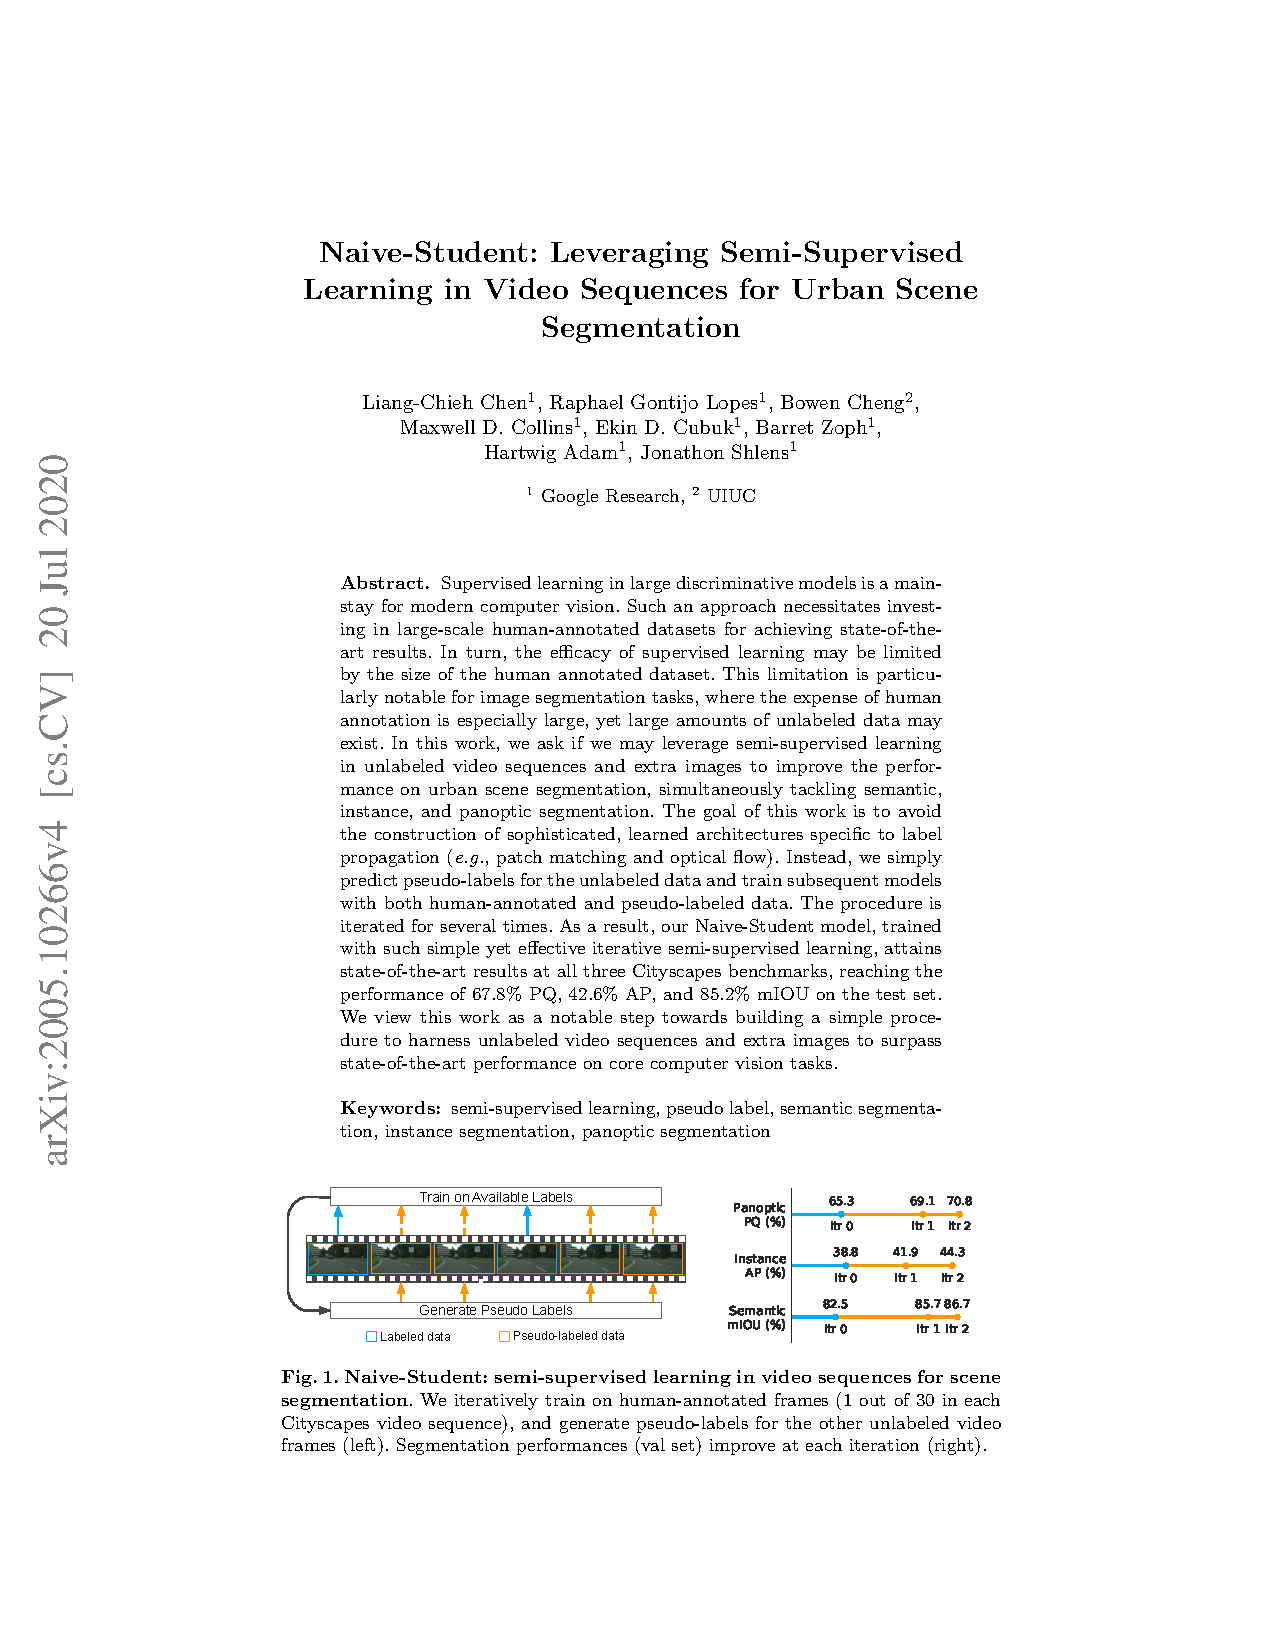
\includegraphics[width=0.8\textwidth]{images/Naive-Student.png} % replace with your image file name
  \caption{Αρχιτεκτονική διαδικασία εκπαίδευσης Naive-Student}
  \label{figure 20}
\end{figure} 

\subsection{State-of-the-art στο σύνολο δεδομένων ADE20K}

\subsubsection{OneFormer}

Το OneFormer~\cite{jain2022oneformertransformerruleuniversal} αποτελεί μοντέλο το οποίο βασίζεται στους μετασχηματιστές και μπορεί να εκτελέσει και τις 3 βασικές εργασίες κατάτμησης εικόνας (Σημασιολογική κατάτμηση, Κατάτμηση αντικειμένων, Πανοπτική κατάτμηση), μέσω μιας ενιαίας αρχιτεκτονικής, ενός ενιαίου μοντέλου και μιας ενιαίας διαδικασίας εκπαίδευσης. Σε αντίθεση με άλλα μοντέλα, τα οποία απαιτούν ξεχωριστή διαδικασία εκπαίδευσης για κάθε εργασία, το OneFormer μπορεί να πραγματοποιήσει και τις 3 βασικές εργασίες κατάτμησης εικόνας μέσω της ίδιας διαδικασίας εκπαίδευσης, μειώνοντας έτσι σημαντικά το υπολογιστικό κόστος, όπως και τον αποθηκευτικό χώρο που θα απαιτούταν. Η αρχιτεκτονική του OneFormer περιλαμβάνει μεταξύ άλλων ένα εξαγωγέα χαρακτηριστικών και ένα αποκωδικοποιητή εικονοστοιχεων, που ο σκοπός τους είναι να εξάγουν χαρακτηριστικά πολλαπλών διαστάσεων απο την εικόνα. Στη συνέχεια, δημιουργούνται queries ανάλογα της εργασία, τα οποία επεξεργάζονται απο τον αποκωδικοποιητή transformer (Transformer decoder). Για την πρόβλεψη το μοντέλο παράγει δυναμικά μάσκες και κατηγορίες ανάλογα με την εργασία που πραγματοποιεί. Στο πλαίσιο της πανοπτικής κατάτμησης εικόνας το OneFormer σε συνδυασμό με τον εξαγωγέα χαρακτηριστικών InternImage-H~\cite{wang2023internimageexploringlargescalevision} πέτυχε πανοπτική ποιότητα ίση με 54.5 στο σύνολο δεδομένων επικύρωσης του ADE20K~\cite{zhou2018semanticunderstandingscenesade20k}.\\

\begin{figure}[h!]
  \centering
  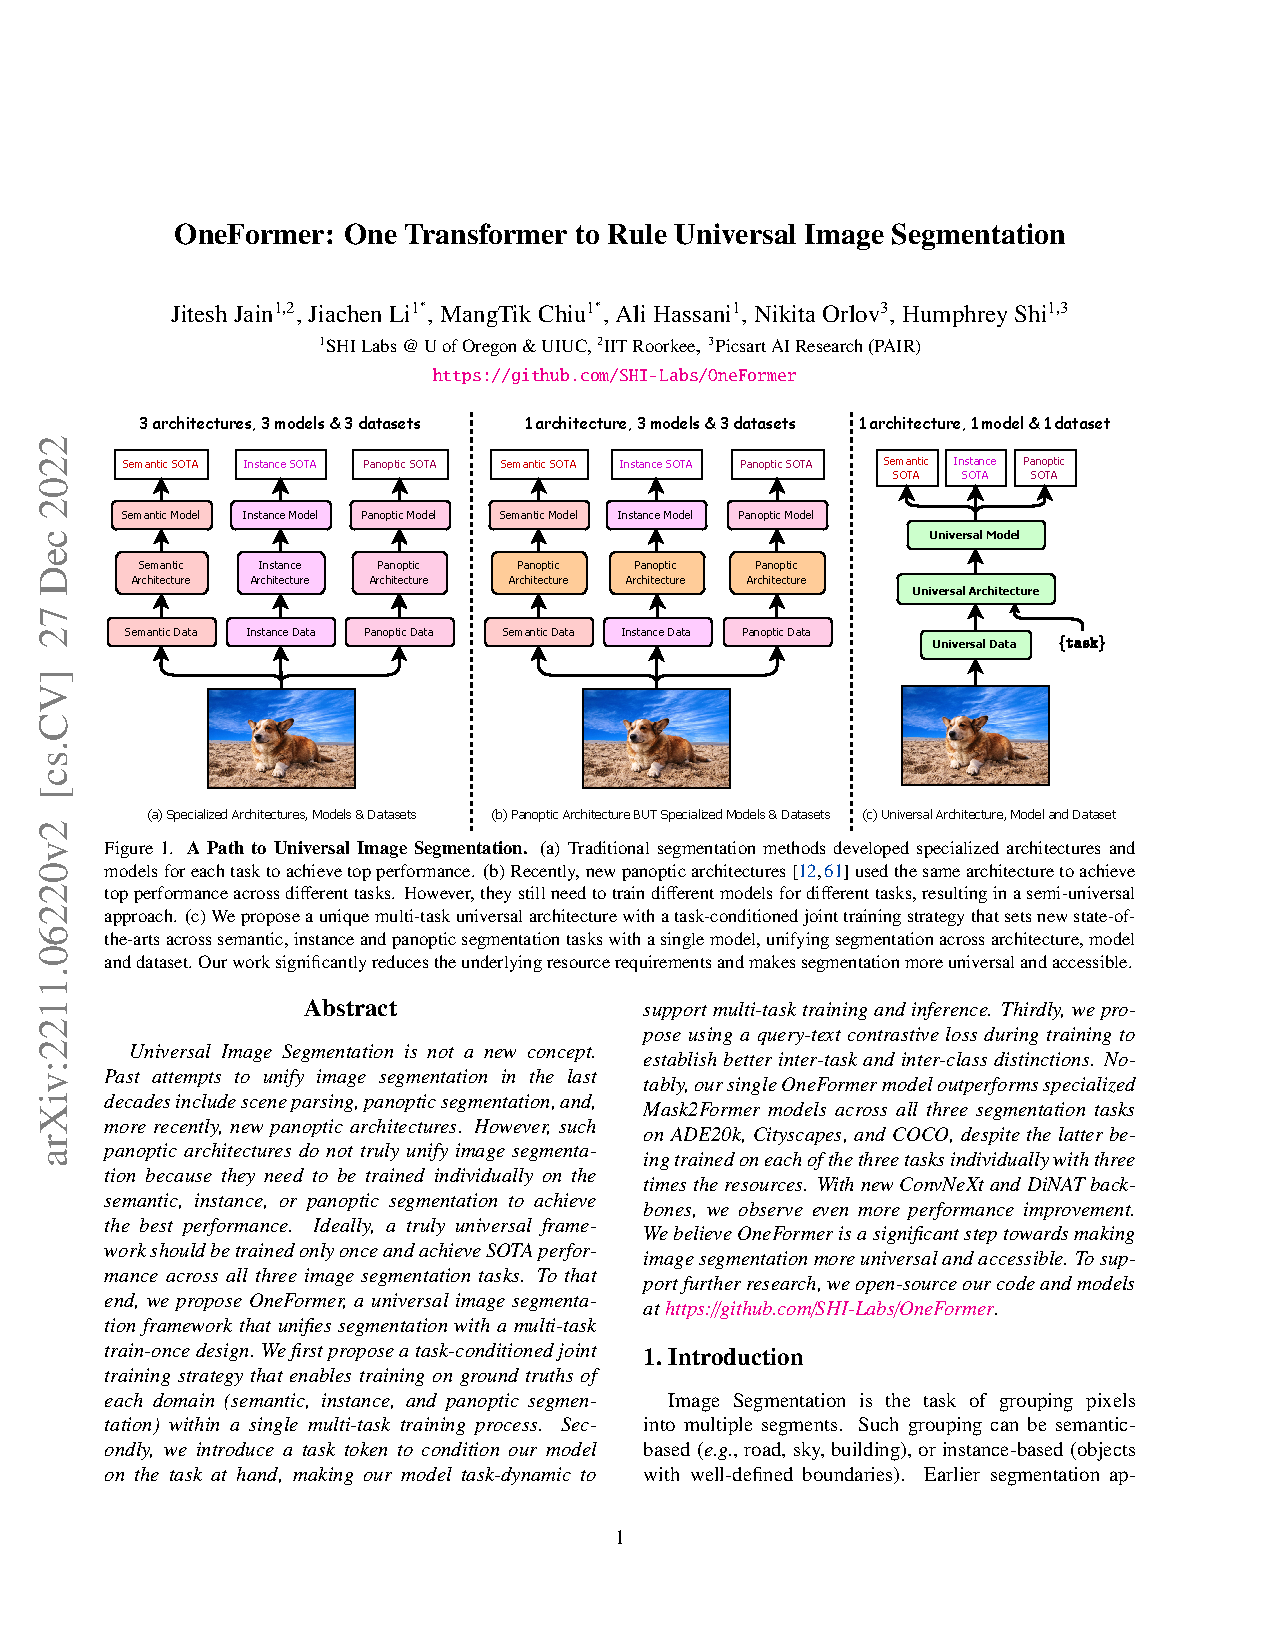
\includegraphics[width=0.9\textwidth]{images/OneFormer.png} % replace with your image file name
  \caption{Αρχιτεκτονική OneFormer}
  \label{figure 20}
\end{figure} 

\subsubsection{OpenSeeD}

Το OpenSeeD~\cite{zhang2023simpleframeworkopenvocabularysegmentation} αποτελεί μια αρχιτεκτονική βασισμένη στους μετασχηματιστές, ικανή να αντιμετωπίσει όλες τις βασικές εργασίες κατάτμησης εικόνας, καθώς και ανίχνευση αντικειμένων. Μπορεί να εκπαιδευτεί τόσο απο δεδομένα ανίχνευσης όσο και απο δεδομένα κατάτμησης, αξιοποιώντας το σύνολο εκπαίδευσης της μίας εργασίας για την εκτέλεση όχι μόνο της ίδιας αλλά και της άλλης. Επιπλέον, μέσω της αρχιτεκτονικής που έχει μπορεί να αναγνωρίζει και να τμηματοποιεί στοιχεία της εικόνας πέρα απο το κλειστό λεξιλόγιο του συνόλου εκπαίδευσης. Η αρχιτεκτονική του αποτελείτε απο ένα κωδικοποιητή εικόνας (Image encoder), ένα κωδικοποιητή κειμένου (Text encoder) και ένα αποκωδικοποιητή που μπορεί να χειριστεί απο "αντικείμενα" και "σκηνικά" στοιχεία, μέχρι και να παράγει τις δυαδικές μάσκες των "αντικειμένων" που προκύπτουν απο τα πλαίσια που περιβάλλουν τα "αντικείμενα" στο σύνολο δεδομένων ανίχνευσης, όλα αυτά μέσω μηχανισμών αυτο-προσοχής και διασταυρούμενης προσοχής. Στο πλαίσιο της πανοπτικής κατάτμησης εικόνας το OpenSeeD σε συνδυασμό με τον εξαγωγέα χαρακτηριστικών Swin-L~\cite{liu2021swintransformerhierarchicalvision} έχει πετύχει πανοπτική ποιότητα ίση με 53.7 στο σύνολο δεδομένων επικύρωσης του ADE20K~\cite{zhou2018semanticunderstandingscenesade20k}.  \\

\begin{figure}[h!]
  \centering
  \includegraphics[width=0.9\textwidth]{images/OpenSeed.png} % replace with your image file name
  \caption{Αρχιτεκτονική OpenSeed}
  \label{figure 20}
\end{figure} 

\subsection{Θεμελιώδεις έρευνες στην πανοπτική κατάτμηση εικόνας}

\subsubsection{Panoptic-DeepLab}

Το Panoptic-DeepLab~\cite{cheng2020panopticdeeplabsimplestrongfast} αποτελεί μοντέλο πανοπτικής κατάτμησης εικόνας. Σε αντίθεση με τα περισσότερα μοντέλα πανοπτικής κατάτμησης της περιόδου αυτής, το Panoptic-DeepLab δεν προσεγγίζει την εργασία απο πάνω πρός τα κάτω (top-down). Η προσέγγιση αυτή ξεκινά με ανίχνευση αντικειμένων και στη συνέχεια κάθε εικονοστοιχείο της εικόνας ανατίθεται σε κάποιο "αντικείμενο" ή "σκηνικό" στοιχείο. Το μοντέλο αυτό προσεγγίζει την εργασία με τρόπο, απο κάτω πρός τα πάνω (bottom-up), δηλαδή ξεκινά με σημασιολογική κατάτμηση εικόνας και στη συνέχεια κάνει διάκριση μεταξύ των "αντικειμένων" που ανήκουν στην ίδια κατηγορία. Συγκεκριμένα, για κάθε εικονοστοιχείο που αντιστοιχεί σε "αντικείμενο" προβλέπει το κέντρο του αντίστοιχου "αντικειμένου", όπως και την μετατόπιση που πρέπει να κάνει για να φτάσει εκεί. Η αρχιτεκτονική του Panoptic-DeepLab αποτελείτε απο 4 βασικά μέρη. Πρώτα χρησιμοποιείτε ένας εξαγωγέας χαρακτηριστικών κωδικοποιητή (Encoder Backbone) ο οποίος αξιοποιείται τόσο στη σημασιολογική κατάτμηση όσο και στην κατάτμηση αντικειμένων. Μετέπειτα αυτού, η διαδικασία χωρίζεται σε 2 διακριτές διακλαδώσεις, με την μία να είναι υπέυθυνη για την εκτέλεση σημασιολογικής κατάτμησης και την άλλη για την εκτέλεση κατάτμησης αντικειμένων. Κάθε διακλάδωση αποτελείτε απο ένα μηχανισμό Atrous Spatial Pyramid Pooling, που έχει ώς σκοπό την εξαγωγή χαρακτηριστικών απο τις εικόνες σε διαφορετικές κλίμακες μέσω διατρητών συνελίξεων, ένα αποκωδικοποιητή ο οποίος προβάλλει τα χαρακτηριστικά του χάρτη χαρακτηριστικών σε υψηλότερες διαστάσεις και μια κεφαλή πρόβλεψης, απο τις οποίες η μια παράγει τον χάρτη σημασιολογικής πρόβλεψης ενώ η άλλη προβλέπει τα κέντρα των "αντικειμένων" και τα διανύσματα μετατόπισης των εικονοστοιχείων πρός αυτά. Τέλος, τα αποτελέσματα των 2 διακλαδώσεων συνδυάζονται για την παραγωγή της πανοπτικής κατάτμησης. \\

\begin{figure}[h!]
  \centering
  \includegraphics[width=0.9\textwidth]{images/Panoptic-DeepLab.png} % replace with your image file name
  \caption{Αρχιτεκτονική μοντέλου Panoptic-DeepLab}
  \label{figure 20}
\end{figure} 

\subsubsection{UPSNet}

Το UPSNet~\cite{xiong2019upsnetunifiedpanopticsegmentation} αποτελεί μοντέλο πανοπτικής κατάτμησης εικόνας. Οι πλειοψηφία των μοντέλων πανοπτικής κατάτμησης που προηγήθηκαν του μοντέλου αυτού βασίζονταν συνήθως στον συνδυασμό των εξόδων ενός μοντέλου σημασιολογικής κατάτμησης εικόνας και της εξόδου ενός μοντέλου κατάτμησης αντικειμένων, μέσω κάποιων προκαθορισμένων κανόνων συνδυασμού, οι οποίοι δεν αποτελούσαν μέρος του μοντέλου αλλά εφαρμόζονταν ώς ξεχωριστό στάδιο επεξεργασίας. Έτσι, ο συνδυασμός αυτός δεν μπορούσε να βελτιστοποιηθεί μέσω εκπαίδευσης, περιορίζοντας έτσι τις δυνατότητες και την ταχύτητα αυτών των συστημάτων. Το UPSNet εισήγαγε μια ενιαία αρχιτεκτονική, η οποία παρόλο που διατήρησε τις διακλαδώσεις των δύο μοντέλων σημασιολογικής κατάτμσησης και κατάτμησης αντικειμένων συνδυάζει τα αποτελέσματα τους μέσω μιας πανοπτικής κεφαλής, επιτρέποντας έτσι ταχύτερη εξαγωγή αποτελεσμάτων. Η αρχιτεκτονική του UPSNet αποτελείτε απο τον εξαγωγέα χαρακτηριστικών, που στην συνέχεια χωρίζεται σε 2 διακλαδώσεις, στην διακλάδωση της σημασιολογικής κατάτμησης εικόνας και στην διακλάδωση της κατάτμησης αντικειμένων. Η διακλάδωση κατάτμησης αντικειμένων αντιστοιχεί στην κεφαλή του Mask R-CNN~\cite{he2018maskrcnn}. Ο εξαγωγέας χαρακτηριστικών είναι ενιαίος για τις 2 εργασίες και βασίζεται στην αρχιτεκτονική των Residual Networks (ResNets)~\cite{he2015deepresiduallearningimage}, όπου σε συνδυασμό με το Feature Pyramid Network~\cite{lin2017featurepyramidnetworksobject} παράγει πολυκλιμακωτά χαρακτηριστικά.Τέλος, τα αποτελέσματα των 2 διακλαδώσεων συνδυάζονται μέσω μιας πανοπτικής κεφαλής, χωρίς παραμέτρους η οποία παράγει την πανοπτική κατάτμηση της εικόνας.  \\

\begin{figure}[h!]
  \centering
  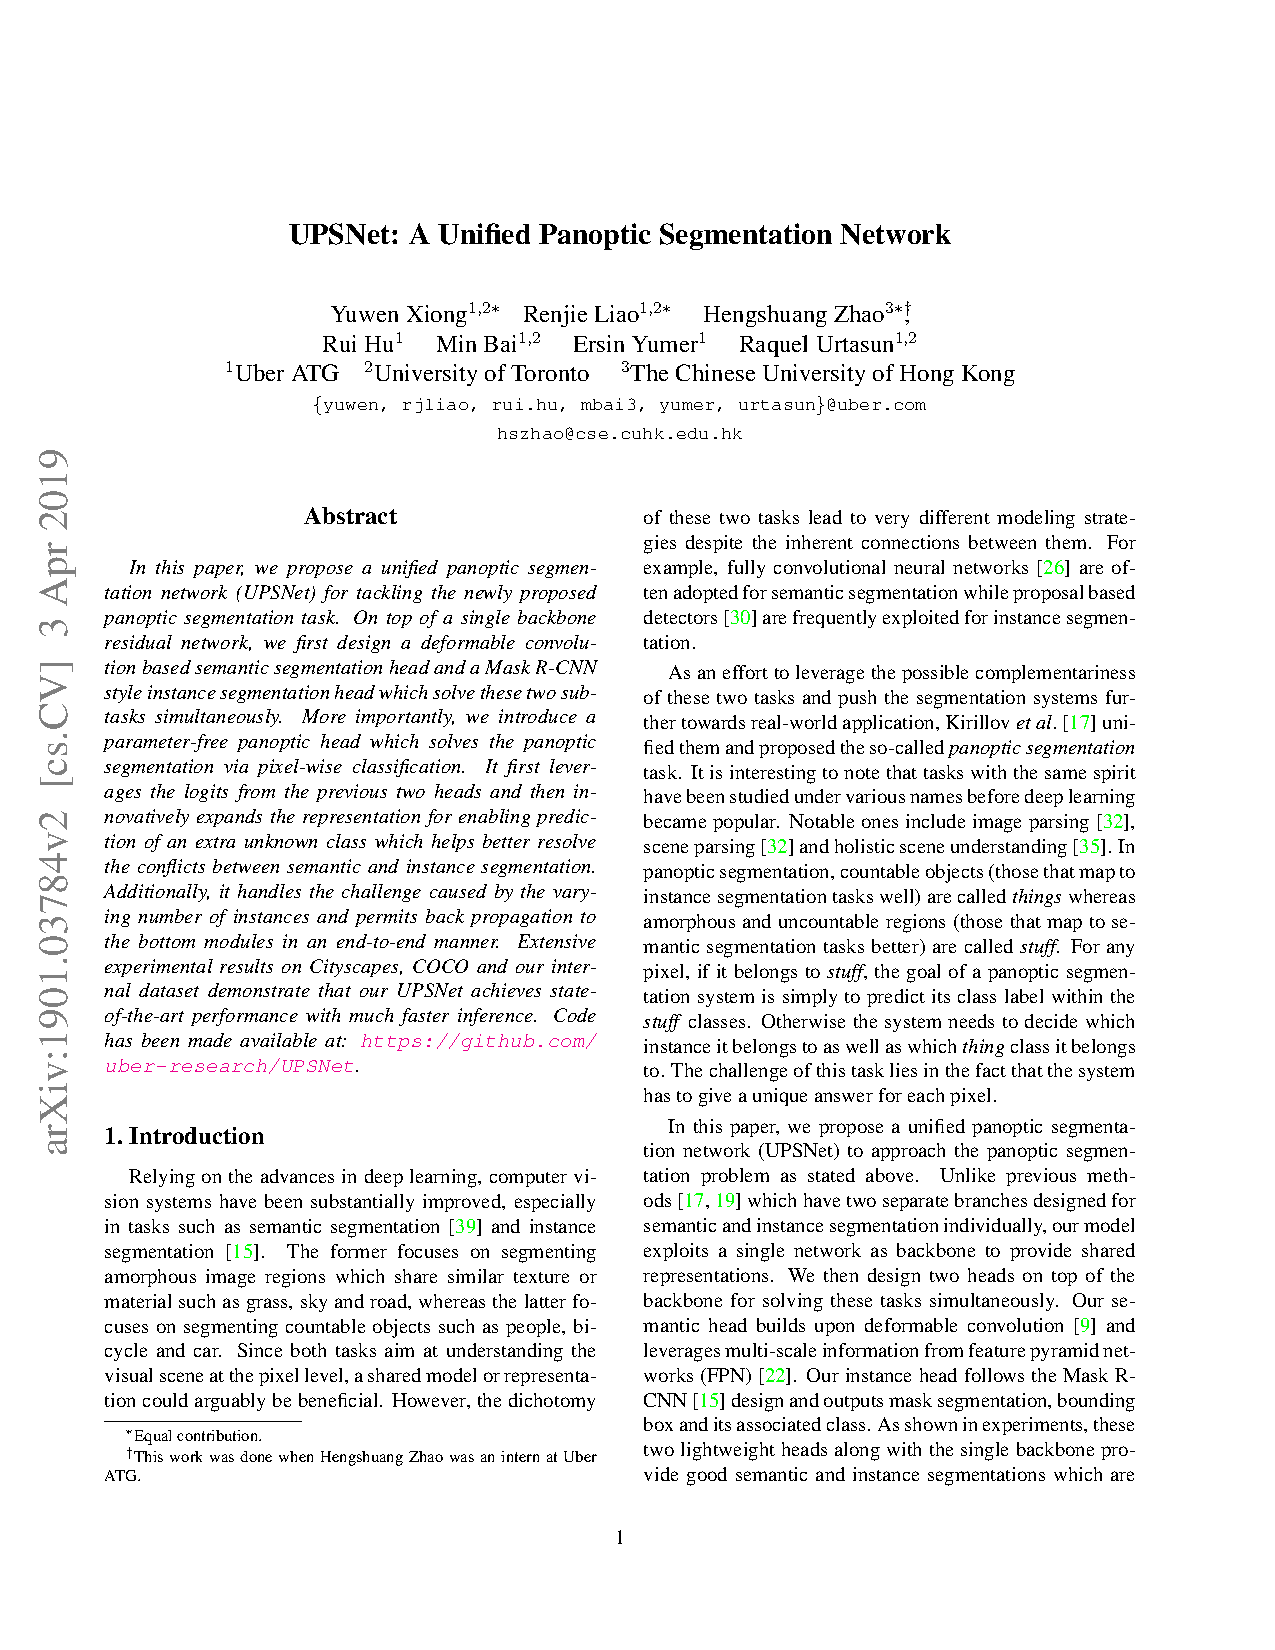
\includegraphics[width=0.9\textwidth]{images/UPSNet.png} % replace with your image file name
  \caption{Αρχιτεκτονική μοντέλου UPSNet}
  \label{figure 20}
\end{figure} 

\subsubsection{Max-DeepLab}

Το Max-DeepLab~\cite{wang2021maxdeeplabendtoendpanopticsegmentation} αποτελεί ένα απο τα σημαντικότερα μοντέλα στην πανοπτική κατάτμηση εικόνας. Τα κλασικά συστήματα της περιόδου αυτής ήταν κυρίως βασισμένα σε διαδικασίες με πολλά ενδιάμεσα βήματα, όπως η ανίχνευση των πλαισίων των "αντικειμένων" και ο συνδυασμός των διαφόρων βημάτων μεταξύ τους, ώστε να παραχθεί το τελικό αποτέλεσμα. Αν και κάθε στάδιο μπορούσε να βελτιστοποιηθεί μεμονωμένα, η προσέγγιση αυτή δεν επέτρεπε την ταυτόχρονη, συνολική βελτιστοποίηση του συστήματος. Το  Max-DeepLab διαφοροποιείτε απο αυτά τα συστήματα εισάγοντας μια ενιαία αρχιτεκτονική κατάτμησης εικόνας, η οποία δεν συμπεριλαβάνει πολύπλοκα ενδιάμεσα στάδια. Η αρχιτεκτονική του περιλαμβάνει ένα μετασχηματιστή διπλής διαδρομής (Dual-Path Transformer), ένα αποκωδικοποιητή και μια κεφαλή εξόδου, η οποία προβλέπει τις μάσκες και κλάσεις της εικόνας εισόδου. Το μοντέλο αποτελείτε απο 2 διακλαδώσεις, την διακλάδωση των εικονοστοιχείων, η οποία εξάγει λεπτομερή χαρακτηριστικά χαμηλού επιπέδου όπως σχήματα και ακμές και την διακλάδωση μνήμης, η οποία εξάγει πληροφορίες απο την εικόνα σε επίπεδο αντικειμένου. Αυτές οι 2 διακλαδώσεις επικοινωνούν μέσω των μετασχηματιστών διπλής διαδρομής. Η διακλάδωση εικονοστοιχείων ενημερώνει την διακλάδωση μνήμης με πιο λεμτομερείς πληροφορίες ενώ η διακλάδωση μνήμης την διακλάδωση εικονοστοιχείων για το ποιο αντικείμενο αντιστοιχεί σε κάθε συνδυασμό σχημάτων, ακμών κ.ο.κ.. Ο αποκωδικοποιητής λειτουργεί συνδυάζοντας χαρακτηριστικά πολλών κλιμάκων της εικόνας και προβάλλοντας τα σε μεγαλύτερες διαστάσεις, με σκοπό την αποκατάσταση των λεπτομερειών και τον σαφή διαχωρισμό των σχημάτων και των ορίων τους στην εικόνα. Τέλος, οι κεφαλές εξόδου αποτελούν το τελευταίο στάδιο του μοντέλου και είναι υπεύθυνες για τη μετατροπή της επεξεργασμένης πληροφορίας σε τελικές προβλέψεις. Συγκεκριμένα, η μία κεφαλή αξιοποιεί τις ενσωματώσεις στην διακλάδωση μνήμης για να αποδώσει σε κάθε στοιχείο την αντίστοιχη κατηγορία, ενώ η άλλη χρησιμοποιεί τα χαρακτηριστικά που παράγονται από τον αποκωδικοποιητή για να καθορίσει ποια εικονοστοιχεία της εικόνας συνδέονται με κάθε κατηγορία. Συνδυάζοντας τις εξόδους των δύο κεφαλών προκύπτει το τελικό αποτέλεσμα.\\

\begin{figure}[H]
  \centering
  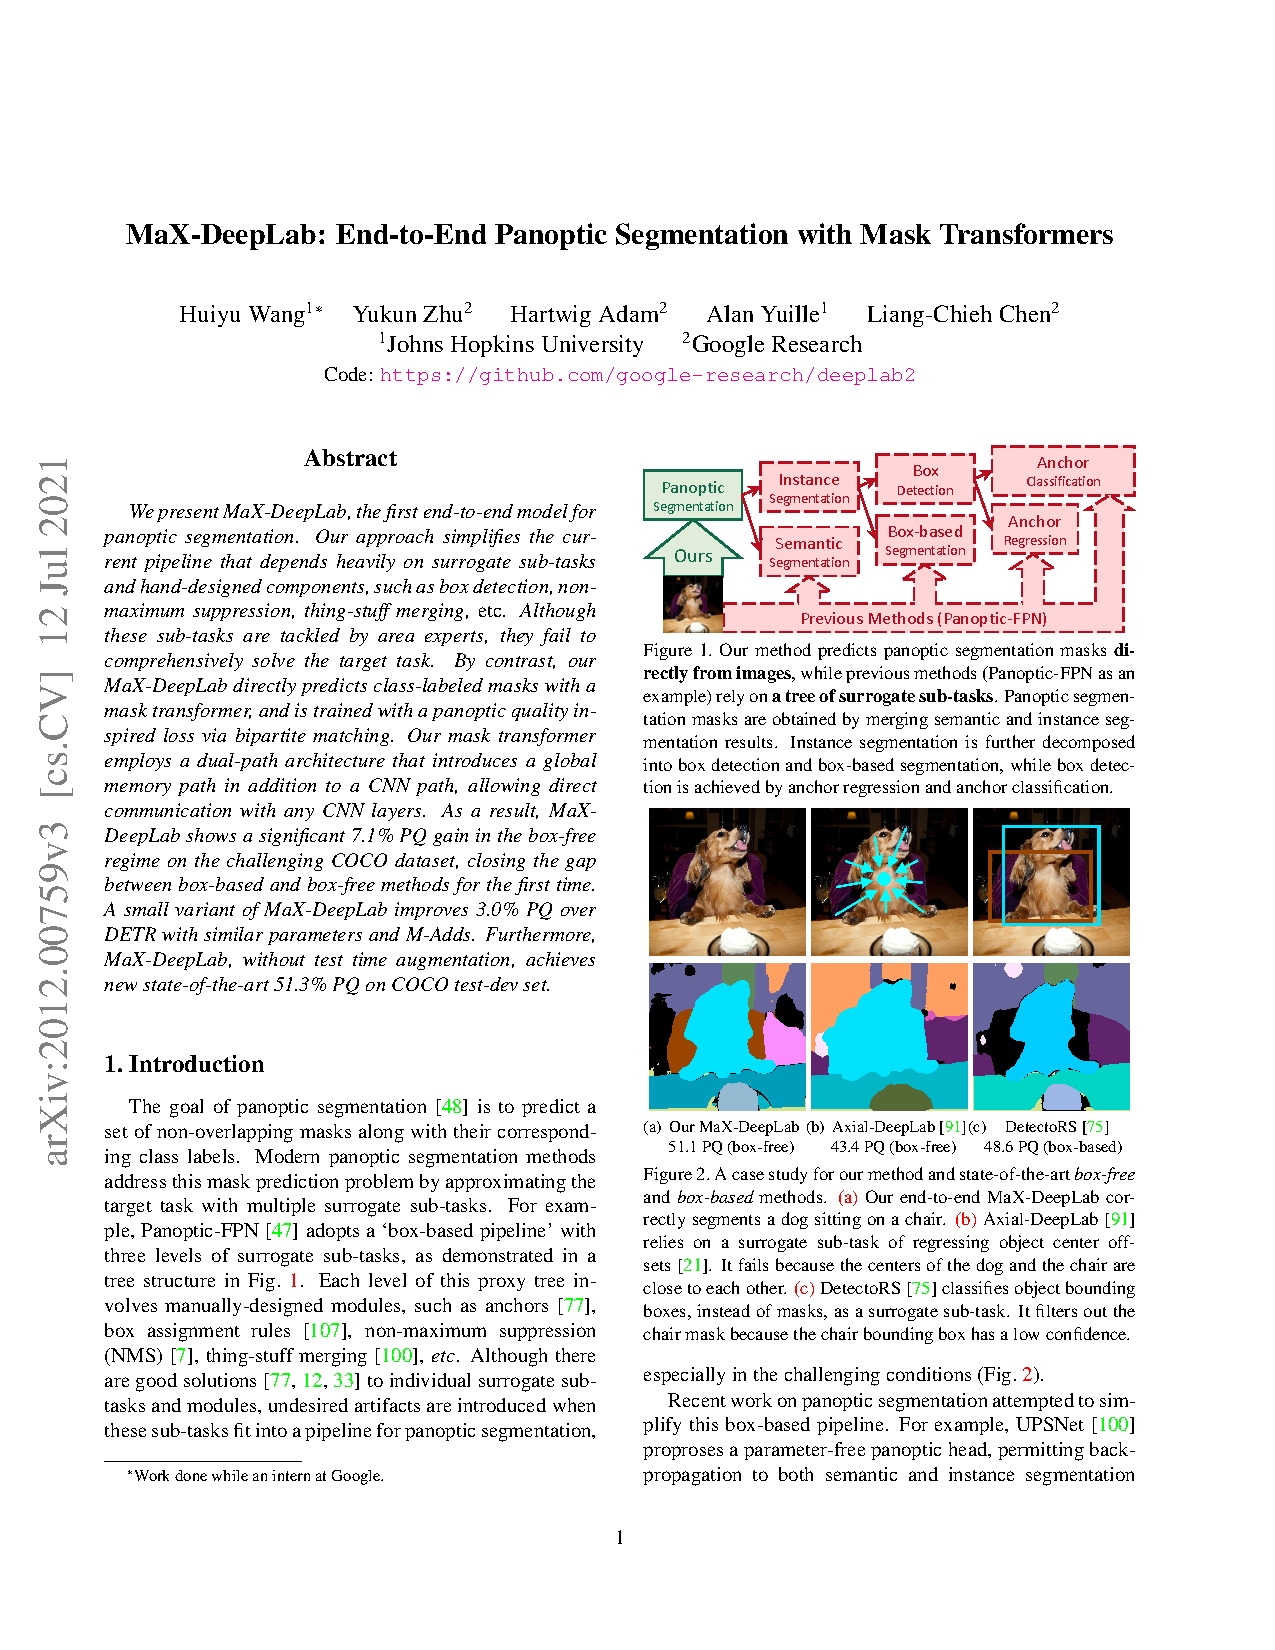
\includegraphics[width=0.6\textwidth]{images/MaxDeepLab.png} % replace with your image file name
  \caption{Αρχιτεκτονική μοντέλου Max-DeepLab}
  \label{figure 20}
\end{figure} 

\clearpage    
\newpage

\section{Συμβολή της εργασίας}

Η εργασία είναι βασισμένη στον εξαγωγέα χαρακτηριστικών Visual Attention Network (VAN). Για τον λόγο αυτό, αρχικά θα παρουσιαστεί εκτενώς η αρχιτεκτονική και τα βασικά του στοιχεία, ώστε να γίνει κατανοητή η λειτουργία του. Στη συνέχεια, θα περιγραφούν αναλυτικά οι τροποποιήσεις και οι επεκτάσεις που υλοποιήθηκαν στο πλαίσιο της παρούσας εργασίας.\\

\subsection{Visual Attention Network - VAN}

Το Visual Attention Network~\cite{guo2022visualattentionnetwork} αποτελεί εξαγωγέα χαρακτηριστικών (Feature Extractor) στην όραση υπολογιστών, σχεδιασμένο για να συνδυάζει τα πλεονεκτήματα των συνελικτικών νευρωνικών δικτύων και των μηχανισμών αυτο-προσοχής, αποφεύγοντας όμως τα μειονεκτήματά τους. Το δίκτυο αυτό δημιουργήθηκε γύρω από έναν νέο μηχανισμό αυτο-προσοχής που ονομάζεται Large Kernel Attention (LKA). Η αυτο-προσοχή, παρόλο που είχε σχεδιαστεί για να αντιμετωπίσει προβλήματα επεξεργασίας φυσικής γλώσσας, στη συνέχεια χρησιμοποιήθηκε ευρέως σε πολλές εργασίες της όρασης υπολογιστών. Ωστόσο, λόγω της δισδιάστατης φύσης των εικόνων, η εισαγωγή της αυτο-προσοχής σε οπτικά δεδομένα συνοδεύτηκε από συγκεκριμένα προβλήματα.\\

\begin{itemize}
    \item Η αντιμετώπιση των εικόνων ως μονοδιάστατες ακολουθίες αγνοεί την δισδιάστατη φύση τους.
    \item Η υπολογιστική πολυπλοκότητα $O(n^2)$ των μηχανισμών αυτο-προσοχής είναι υπερβολικά υψηλή για εικόνες υψηλής ανάλυσης.
    \item Οι συμβατικοί μηχανισμοί αυτο-προσοχής εστιάζουν αποκλειστικά στη χωρική αλληλεπίδραση μεταξύ των εικονοστοιχείων, αγνοώντας τη σημασία της αλληλεπίδρασης μεταξύ διαφορετικών καναλιών. Συχνά, διαφορετικά κανάλια σε μια εικόνα αναπαριστούν διαφορετικά αντικείμενα.
\end{itemize}

Λύση στα παραπάνω προβλήματα επιχειρεί να δώσει ο Large Kernel Attention που παρόλο που μπορεί να λειτουργεί ώς μηχανισμός αυτο-προσοχής, δεν κληρονομεί τα αντίστοιχα προβλήματα. Η βασική ιδέα πίσω απο αυτό αποτελεί η χρήση συνέλιξης μεγάλου πυρήνα έτσι ώστε να μπορούμε να υπολογίσουμε τις σχέσεις μεταξύ εικονοστοιχείων που έχουν μεγάλη απόσταση μεταξύ τους και στην συνέχεια να κατασκευάσουμε τον χάρτη προσοχής (Attention map). Ωστόσο, η χρήση συνέλιξης με μεγάλο πηρύνα απαιτεί μεγάλη υπολογιστική πολυπλοκότητα και σημαντικό αριθμό παραμέτρων. Για την αντιμετώπιση αυτού του προβλήματος το Large Kernel Attention χρησιμοποιεί μια αποσυντεθειμένη μορφή της συνέλιξης έτσι ώστε να αποφευχθεί η μεγάλη υπολογιστική πολυπλοκότητα που απατείται. Συγκεκριμένα, μια συνελικτική πράξη μπορεί να αποσυντεθεί σε τρία μέρη, μια χωρική συνέλιξη μικρών διαστάσεων για την καταγραφή των τοπικών συσχετίσεων, μια διευρυμένη χωρική συνέλιξη για την καταγραφή μακρινών σχέσεων και μια συνελικτική πράξη μεταξύ των καναλιών, η οποία καταγράφει την συσχέτιση μεταξύ των καναλιών. \\

\noindent Πιο συγκεκριμένα, με βάση το ~\cite{guo2022visualattentionnetwork} μια συνελικτική πράξη με μεγάλο πηρύνα διαστάσεων K x K αποσυντίθεται σε μια \(\left\lceil \frac{K}{d} \right\rceil \times \left\lceil \frac{K}{d} \right\rceil\) χωρική συνέλιξη με συντελεστή απόστασης d, μια (2d - 1) x (2d - 1) χωρική συνέλιξη και μια 1 x 1 συνέλιξη η οποία λαμβάνει την συσχέτιση μεταξύ των καναλιών. Μέσω αυτής της αποσύνθεσης δύναται να ληφθούν συσχετίσεις μεταξύ στοιχείων που έχουν μεγάλη απόσταση μεταξύ τους χωρίς όμως να επιβαρύνεται σημαντικά η υπολογιστική πολυπλοκότητα ή να αυξάνεται ο αριθμός των παραμέτρων του μοντέλου.  \\

\begin{figure}[h!]
  \centering
  \includegraphics[width=0.6\textwidth]{images/LKA.png} % replace with your image file name
  \caption{Αποσύνθεση συνελικτικών πράξεων LKA για K = 7 και d = 2}
  \label{figure 20}
\end{figure} 

\noindent Η μέθοδος που περιγράφηκε παραπάνω μπορεί να γραφεί με τρόπο που φαίνετε στην συνέχεια. \\

\begin{equation}
\textit{Attention} = \text{Conv}_{1 \times 1}(\text{DW-D-Conv}(\text{DW-Conv}(F)))
\end{equation}\\

\begin{equation}
\textit{Output} = \textit{Attention} \otimes F
\end{equation}\\

\noindent όπου F \(\in \mathbb{R}^{C x H x W}\) η είσοδος. Ισχύει πως Attention \(\in \mathbb{R}^{C x H x W}\) και αντιστοιχεί στον χάρτη προσοχής (Attention Map). Η τιμή σε κάθε θέση του χάρτη εκφράζει το πόσο σημαντικό είναι το αντίστοιχο χαρακτηριστικό. Ο τελεστής \( \otimes \) αντιστοιχεί στον πολλαπλασιασμό ανά στοιχείο. \\

Στη συνέχεια θα ορίσουμε το Visual Attention Network. Ο μηχανισμός LKA που περιγράψαμε παραπάνω αποτελεί επιμερές στοιχείο του VAN. Το VAN αποτελείτε απο 4 στάδια. Έστω H x W οι χωρικές διαστάσεις της εικόνας εισόδου. Πρίν απο κάθε στάδιο οι χωρικές διαστάσεις της εισόδου μειώονονται μέσω μιας συνελικτικής πράξης με βήμα. Η μείωση των χωρικών διαστάσεων εξαρτάται απο το στάδιο το οποίο βρίσκεται το μοντέλο. Συγκεκριμένα, οι χωρικές διαστάσεις της εικόνας μειώνονται πρίν απο το πρώτο στάδιο σε \(\frac{H}{4} x \frac{W}{4}\), πρίν απο το δεύτερο σε \(\frac{H}{8} x \frac{W}{8}\), πρίν απο το τρίτο σε \(\frac{H}{16} x \frac{W}{16}\) και πρίν απο το τέταρτο σε \(\frac{H}{32} x \frac{W}{32}\). Ο αριθμός των καναλιών C εξαρτάται απο τον τύπο VAN που χρησιμοποιείτε. Υπάρχουν 7 διαφορετικοί τύποι VAN. Ενδεικτικά για το VAN-B0 έχουμε στο πρώτο στάδιο C = 32, στο δεύτερο C = 64, στο τρίτο C = 160 και στο τέταρτο C = 256. Μετά την μείωση των διαστάσεων της εισόδου, καθόλη την διάρκεια του σταδίου τόσο οι χωρικές διαστάσεις όσο και η διάσταση των καναλιών C παραμένουν σταθερές. Μετά απο κάθε μείωση διαστάσεων της εισόδου, η έξοδος περνά μέσα απο L διαδοχικές ομάδες όπου η κάθε μια περιλαμβάνει στοιχεία όπως κανονικοποίηση παρτίδας, συνελίξεις, συνάρτηση ενεργοποίησης GeLU, μηχανισμό προσοχής και πλήρως συνδεδεμένο δίκτυο. Οι L αυτές ομάδες συγκροτούν ένα πλήρες στάδιο του Visual Attention Network. Ο αριθμός L εξαρτάται απο το παρών στάδιο όπως και απο τον τύπο του μοντέλου VAN που χρησιμοποιείτε. Ενδεικτικά για το VAN-B0 στο πρώτο και στο δεύτερο στάδιο ορίζεται η τιμή L = 3, στο τρίτο L = 5 και στο τέταρτο L = 2. Ένα πλήρες στάδιο VAN παρουσιάζεται στην εικόνα παρακάτω.\\

\begin{figure}[h!]
  \centering
  \includegraphics[width=0.6\textwidth]{images/VAN_Stage.png} % replace with your image file name
  \caption{Αρχιτεκτονική ενός σταδίου του VAN}
  \label{figure 20}
\end{figure} 

\noindent Στο συγκεκριμένο άρθρο χρησιμοποιείτε η τιμή K = 21 ώς προεπιλογή. Για την τιμή αυτή το πληθος των παραμέτρων ελαχιστοποιείτε ορίζοντας d = 3. Ο συνδυασμός αυτός αντιστοιχεί σε μια 5 x 5 χωρική συνέλιξη και μια 7 x 7 χωρική συνέλιξη με συντελεστή απόστασης ίσο με 3.\\

\newpage

\renewcommand{\refname}{Βιβλιογραφική αναφορά}
\bibliographystyle{ieeetr}  % or another style like plain, alpha, apalike
\bibliography{references}



 

\end{document}
